\documentclass[12pt,a4paper]{article}
\usepackage[utf8]{vietnam}
\usepackage{amsmath}
\usepackage{amsfonts}
\usepackage{amssymb}
\usepackage{tikz, tkz-euclide, tkz-tab}
\usepackage{pgf,pgfplots}
\pgfplotsset{compat=1.15}
\usetikzlibrary{calc,intersections,patterns,arrows,shapes}
\usepackage{graphicx}
\usepackage[unicode]{hyperref}
\usepackage[left=2cm,right=2cm,top=2cm,bottom=2cm]{geometry}
\begin{document}
\begin{center}
\textbf{TRƯỜNG THPT CHUYÊN LÊ QUÝ ĐÔN - BÀ RỊA - VŨNG TÀU}\\
\textbf{LỚP 10 TOÁN 1 (2017-2018)}\\
\end{center}
\begin{center}
\fontsize{20}{18}\selectfont
Chuyên đề\\
\textbf{TỨ GIÁC ĐIỀU HÒA VÀ ỨNG DỤNG GIẢI TOÁN HÌNH HỌC}
\end{center}
\begin{center}
\begin{tikzpicture}
	\draw [ultra thick] (-3,3)node [above left] {$A$}--(5,5)node [above 		right] {$B$};
	\draw [ultra thick] (5,5)--(8,-2)node [below right] {$C$};
	\draw [ultra thick] (8,-2)--(-5,-2)node [below left] {$D$};
	\draw [ultra thick] (-5,-2)--(-3,3);
\end{tikzpicture}
\end{center}
\begin{flushright}
Vũng Tàu, tháng 11 - 12 năm 2017
\end{flushright}
\textbf{Giáo viên hướng dẫn:} Thầy Trần Quang Vinh, Giáo viên trường THPT Chuyên Lê Quý Đôn.\\
\textbf{Học sinh thực hiện:}
Lê Khánh Duy\\
Nguyễn Mai Gia Hân\\
Nguyễn Văn Lộc\\
\newpage
\tableofcontents
\newpage
\section{Lời mở đầu}
\textit{Tứ giác điều hòa là một tứ giác nội tiếp đặc biệt, thú vị trong hình học, do đó nó là một chủ đề không thể thiếu trong hình học Euclide cổ điển (nếu coi đường thẳng là đường tròn suy rộng thì tứ giác điều hòa là một khái niệm xuất phát từ hàng điểm điều hòa, tỉ số kép. Tứ giác điều hòa có ứng dụng khá lớn trong các bài toán định tính như chứng minh thẳng hàng, đồng quy, song song, vuông góc, trung điểm, chứng minh đi qua điểm cố định và các bài toán về chứng minh hệ thức trong hình học... Đây là một công cụ xuất sắc mà bất kì người yêu Toán nào cũng nên biết và nắm vững, được sử dụng để mang đến nhiều lời giải "đẹp". Rất nhiều các bài toán hình học trong các cuộc thi Olympic Toán gần đây chứa đựng trong nó các ý tưởng về tứ giác điều hòa. Chính vì vậy nhóm chúng em đã nghiên cứu và viết thành chuyên đề này với hi vọng đem lại cho bạn đọc đầy đủ những ứng dụng của tứ giác điều hòa.}
\begin{flushright}
\textbf{Nhóm tác giả}
\end{flushright}
\newpage
\section{Kiến thức chuẩn bị.}
\subsection{Các kiến thức cơ bản về véc-tơ, độ dài đại số, các định lí cơ bản.}
\subsection{Hàng điểm điều hòa và chùm điều hòa.}
\subsubsection{Hàng điểm điều hòa.}
Cho bốn điểm \(A, B, C, D\) phân biệt trên trục. Ta định nghĩa tỉ số kép \(\left( {ABCD} \right)\) là \(\frac{{\overline {AC} }}{{\overline {AD} }}:\frac{{\overline {BC} }}{{\overline {BD} }}.\)\\
Nếu \(\left( {ABCD} \right) =  - 1\) thì ta nói \(A, B, C, D\) lập thành hàng điểm điều hòa.\\
\textbf{\textit{*Hai dạng hàng điểm điều hòa cơ bản.}}\\
i. Cho tam giác \(ABC\) không cân có phân giác \(AD, AE\) \(\left( {D,E \in BC} \right)\) thì ta có: \(\left( {EDBC} \right) =  - 1.\)
\begin{center}
	\begin{tikzpicture}
	\draw(-4,4)node [above] {$A$}--(-2,0)node [below] {$B$};
	\draw(-2,0)--(6,0)node [below] {$C$}--(-4,4);
	\draw(-4,4)--(0.35,0)node [below] {$D$};
	\draw(-4,4)--(-7.68,0)node [below] {$E$}--(-2,0);
	\end{tikzpicture}
\end{center}
ii. Tứ giác \(ABCD\) có \(AB\) cắt \(CD\) tại \(F\), \(AD\) cắt \(BC\) tại \(E\), \(AC\) cắt \(BD\) tại \(I\), \(EI\) cắt \(CD\) tại \(K\). Khi đó: \(\left( {FKDC} \right) =  - 1.\) 
\begin{center}
	\begin{tikzpicture}
	\draw(-3,2)node [above left] {$A$}--(3,5)node [above right] {$B$}--(6,0)node [below right] {$C$}--(-5,0)node [below left] {$D$}--(-3,2);
	\draw(6,0)--(1.88,6.88)node [above] {$E$}--(-5,0);
	\draw(3,5)--(-7,0)node [above left] {$F$}--(6,0);
	\draw(1.88,6.88)--(-3.53,0)node [below]  {$K$}--(-2.11,1.8)node  [below] {$I$};
	\draw(-3,2)--(6,0);
	\draw(3,5)--(-5,0);
	\end{tikzpicture}
\end{center}
\textbf{\textit{*Một vài dấu hiệu nhận biết hàng điểm điều hòa.}}\\
Cho \(A\left( a \right);B\left( b \right);C\left( c \right);D\left( d \right)\) trên trục. Khi đó \(\left( {ABCD} \right) =  - 1\) khi và chỉ khi một trong các điều kiện sau được thỏa mãn:
i. \(\left( {a + b} \right)\left( {c + d} \right) = 2\left( {ab + cd} \right)\) (Lagrange).\\
ii. \(\frac{1}{{\overline {AC} }} + \frac{1}{{\overline {AD} }} = \frac{2}{{\overline {AB} }}\) (Descartes).\\
iii. \(\overline {MC} .\overline {MD}  = M{A^2}\) với \(M\) là trung điểm \(AB\) (Newton).\\\
iv. \(\overline {AC} .\overline {AD}  = \overline {AB} .\overline {AI} \) với \(I\) là trung điểm \(CD\) (Maclaurin).\\
\textbf{\textit{*Phép chiếu xuyên tâm bảo toàn hàng điểm điều hòa.}}\\
Cho \(\left( {ABCD} \right) =  - 1\) và điểm \(S \notin \left( {ABCD} \right).\) Đường thẳng \(d\) bất kì không qua \(S\) cắt \(SA, SB, SC, SD\) lần lượt tại \(A_1, B_1, C_1, D_1\). Khi đó \(\left( {{A_1}{B_1}{C_1}{D_1}} \right) =  - 1.\)
\subsubsection{Chùm điều hòa.}
Cho \(\left( {ABCD} \right) =  - 1\) và điểm \(S \notin \left( {ABCD} \right).\) Bốn đường \(SA, SB, SC, SD\) lập thành chùm điều hòa đỉnh \(S\). \\
Kí hiệu: \(\left( {SA,SB,SC,SD} \right) =  - 1\) hoặc \(S\left( {ABCD} \right) =  - 1.\)
\textbf{\textit{*Hai dạng chùm điều hòa cơ bản.}}\\
\textit{i. Chùm trung tuyến.} Cho tam giác \(ABC\) có \(M\) là trung điểm \(BC\), \(Ad\) song song với \(BC\). Khi đó: \(\left( {AB,AC,AM,Ad} \right) =  - 1.\)
\begin{center}
	\begin{tikzpicture}
	\draw(-1,4)node [above left] {$A$}--(-3,-1)node [below left] 
	{$B$}--(4,-1)node [below right] {$C$}--(-1,4);
	\draw(-1,4)--(0.5,-1)node [below] {$M$};
	\draw(-1,4)--(4,4)node [above right] {$d$};
	\end{tikzpicture}
\end{center}
\textit{ii. Chùm phân giác.} Cho \(Sb, Sd\) là hai tia phân giác của góc \(\widehat {aSc}\). Khi đó: \(S\left( {abcd} \right) =  - 1.\)
\begin{center}
	\begin{tikzpicture}
	\draw(-1,4)node [above left] {$S$}--(-3,-1)node [left] 
	{$a$};
	\draw(-1,4)--(4,-1)node [right] {$c$};
	\draw(-1,4)--(0.03,-1)node [above left] {$b$};
	\draw(-1,4)--(4,5.03)node [above right] {$d$};
	\end{tikzpicture}
\end{center}
\subsection{Tỉ số kép với góc định hướng.}
\textit{Định lí 1 (Định lí Ceva dạng lượng giác).} Cho tam giác \(ABC\) và các điểm \(M, N, P\) theo thứ tự thuộc các đường thẳng \(BC, CA, AB\) (nhưng không trùng với đỉnh của tam giác). Khi đó, \(AM, BN, CP\) đồng quy hoặc đôi một song song nếu và chỉ nếu \(\frac{{\sin \left( {\overrightarrow {AM} ;\overrightarrow {AB} } \right)}}{{\sin \left( {\overrightarrow {AM} ;\overrightarrow {AC} } \right)}}.\frac{{\sin \left( {\overrightarrow {BN} ;\overrightarrow {BC} } \right)}}{{\sin \left( {\overrightarrow {BN} ;\overrightarrow {BA} } \right)}}.\frac{{\sin \left( {\overrightarrow {CP} ;\overrightarrow {CA} } \right)}}{{\sin \left( {\overrightarrow {CP} ;\overrightarrow {CB} } \right)}} = 1.\)\\
\textit{Hệ quả:} Khi \(M, N, P\) theo thứ tự thuộc các đường thẳng \(BC, CA, AB\) và không trùng với hai đầu mút của các đoạn thẳng này thì \(AM, BN, CP\) đồng quy khi và chỉ khi \(\frac{{\sin \widehat {MAB}}}{{\sin \widehat {MAC}}}.\frac{{\sin \widehat {NBC}}}{{\sin \widehat {NBA}}}.\frac{{\sin \widehat {PCA}}}{{\sin \widehat {PCB}}} = 1.\)\\
\textit{Định lí 2.} Với mọi chùm \(O\left( {ABCD} \right)\), ta có \(O\left( {ABCD} \right) = \frac{{\sin \left( {\overrightarrow {OC} ;\overrightarrow {OA} } \right)}}{{\sin \left( {\overrightarrow {OC} ;\overrightarrow {OB} } \right)}}:\frac{{\sin \left( {\overrightarrow {OD} ;\overrightarrow {OA} } \right)}}{{\sin \left( {\overrightarrow {OD} ;\overrightarrow {OB} } \right)}}.\)\\
\textit{Tỉ số kép với góc định hướng.} Cho bốn điểm phân biệt \(A, B, C, D\) cố định trên đường tròn \(\left( O \right)\) và điểm \(M\) thay đổi trên \(\left( O \right)\) thì \(M\left( {ABCD} \right)\) không đổi (khi \(M\) trùng với \(A, B, C, D\) thì \(MA, MB, MC, MD\) tương ứng được coi là tiếp tuyến của \(\left( O \right)\) tại \(A, B, C, D\)). 
\newpage
\section{Tứ giác điều hòa.}
\subsection{Định nghĩa.} Tứ giác nội tiếp \(ABCD\) được gọi là tứ giác điều hòa nếu tồn tại điểm \(M\) thuộc đường tròn ngoại tiếp tứ giác sao cho \(M\left( {ABCD} \right) =  - 1\), cũng tức là \(\left( {ABCD} \right) =  - 1\).\\
Như vậy, nếu tứ giác \(ABCD\) là tứ giác điều hòa thì \(M\left( {ABCD} \right) =  - 1\) với mọi điểm \(M\) thuộc đường tròn ngoại tiếp tứ giác.
\subsection{Tính chất.} 
Cho tứ giác \(ABCD\) nội tiếp đường tròn \(\left( O \right)\). Gọi \({\Delta _a},{\Delta _b},{\Delta _c},{\Delta _d}\) lần lượt là tiếp tuyến với \(\left( O \right)\) tại \(A, B, C, D\). Khi đó, các điều kiện sau đây là tương đương:\\
a. Tứ giác \(ABCD\) là tứ giác điều hòa.\\
b. \(AB.CD = AD. BC\).\\
c. \({\Delta _a}, {\Delta_c}, BD\) đồng quy và \({\Delta_b}, {\Delta_d}, AC\) đồng quy.\\
d. Các phân giác của các góc \(\widehat {BAD},\widehat {BCD}\) cắt nhau tại một điểm trên đường chéo \(BD\), các phân giác của các góc \(\widehat {ABC},\widehat {ADC}\) cắt nhau tại một điểm trên đường chéo \(AC\).\\
e. \(\widehat {MAD} = \widehat {BCA}\) với \(M\) là trung điểm \(BD\). Tương tự với trung điểm \(AC\).
\subsection{Chứng minh tính chất.}
\begin{center}
	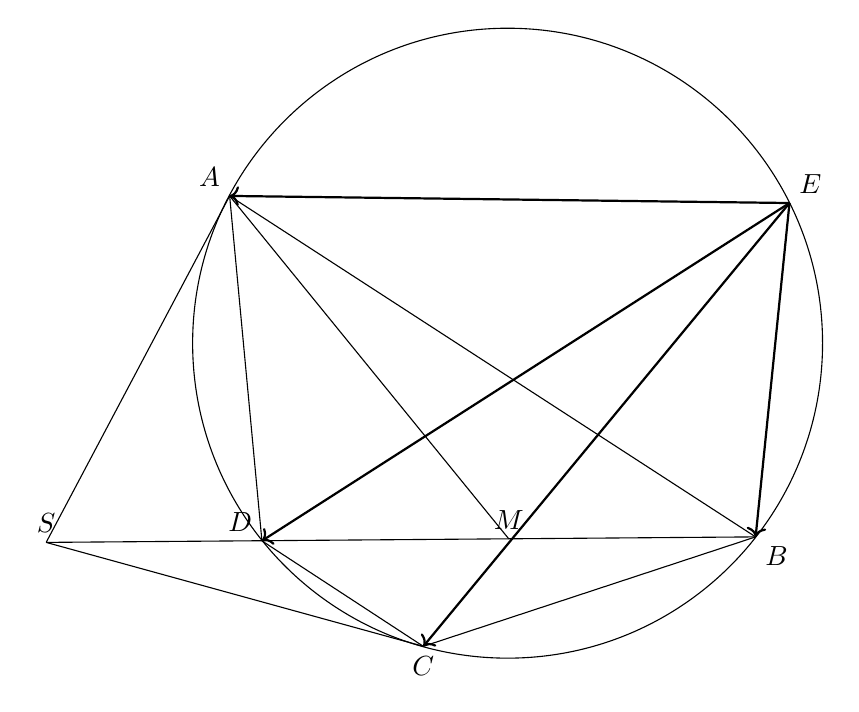
\begin{tikzpicture}
	\draw (-2,2) circle [radius = 4];;
	\draw (-5.53,3.87)node [above left] {$A$}--(1.15,-0.46)node [below 		 	right] {$B$};
	\draw (1.15,-0.46)--(-3.07,-1.85)node [below] {$C$};
	\draw (-3.07,-1.85)--(-5.12,-0.51)node [above left] {$D$};
	\draw (-5.12,-0.51)--(-5.53,3.87);
	\draw (-7.86,-0.53)node [above] {$S$}--(-5.53,3.87);
	\draw (-7.86,-0.53)--(-3.07,-1.85);
	\draw (-7.86,-0.53)--(1.15,-0.46);
	\draw (1.58,3.78)node [above right] {$E$};
	\draw [->] [thick] (1.58,3.78)--(-5.53,3.87);
	\draw [->] [thick] (1.58,3.78)--(1.15,-0.46);
	\draw [->] [thick] (1.58,3.78)--(-3.07,-1.85);
	\draw [->] [thick] (1.58,3.78)--(-5.12,-0.51);
	\draw (-1.985,-0.485)node [above] {$M$};
	\draw (-1.985,-0.485)--(-5.53,3.87);
	\end{tikzpicture}
\end{center}
\(*\left( {a \Leftrightarrow b} \right)\) Lấy \(E\) bất kì trên \(\left( O \right)\). Tứ giác \(ABCD\) là tứ giác điều hòa. \\
\( \Leftrightarrow E\left( {ABCD} \right) =  - 1\) (theo định nghĩa tứ giác điều hòa).\\
\( \Leftrightarrow \frac{{\sin \left( {\overrightarrow {EB} ;\overrightarrow {EA} } \right)}}{{\sin \left( {\overrightarrow {EB} ;\overrightarrow {EC} } \right)}}:\frac{{\sin \left( {\overrightarrow {ED} ;\overrightarrow {EA} } \right)}}{{\sin \left( {\overrightarrow {ED} ;\overrightarrow {EC} } \right)}} =  - 1.\)\\
\( \Leftrightarrow \frac{{BA}}{{BC}} = \frac{{DA}}{{DC}}\) (theo định lí hàm số sin).\\
\( \Leftrightarrow AB.CD = AD.CB.\)\\
\(*\left( {b \Leftrightarrow c} \right)\)\\
\(\left( {c \Rightarrow b} \right)\) Gọi \(S\) là điểm đồng quy của \({\Delta _a}, {\Delta_c}, BD\).\\
Hai tam giác \(SAB\) và \(SDA\) đồng dạng, hai tam giác \(SCB\) và \(SDC\) đồng dạng.\\
Suy ra: \(\frac{{AB}}{{DA}} = \frac{{SA}}{{SD}};\frac{{CB}}{{DC}} = \frac{{SC}}{{SD}}\)\\
Mà \(SA = SC\) \( \Rightarrow \frac{{AB}}{{DA}} = \frac{{CB}}{{DC}} \Rightarrow AB.CD = AD.BC.\)\\
\(\left( {b \Rightarrow c} \right)\) Gọi \(S\) là giao điểm của \({\Delta _a}\) và \({\Delta _c}.\)\\
Gọi \(D'\) là giao điểm của tia \(SB\) và cung $\stackrel\frown{AC}$ (chứa \(D\)) của đường tròn \(\left( O \right)\).\\
Suy ra: \({\Delta _a},{\Delta _c},BD'\) đồng quy tại \(S\). Do đó, theo \(\left( {c \Rightarrow b} \right)\), ta có: \(AB.CD' = AD'.CB\).\\
Mặt khác, do \(AB.CD = AD.BC\) nên \(\frac{{CD'}}{{CD}} = \frac{{AD'}}{{AD}}\), mà \(D\) và \(D'\) cùng thuộc cung $\stackrel\frown{AC}$ (không chứa \(B\)) nên \(\widehat {ADC} = \widehat {AD'C}.\) Do đó, hai tam giác \({ADC}\) và \({AD'C}\) đồng dạng.\\
Từ đó, tương tự như trên, ta có \(D'\) trung với \(D\) nên \(S, B, D\) thẳng hàng.\\
Vậy \({\Delta _a}, {\Delta_c}, BD\) đồng quy. Tương tự với \({\Delta_b}, {\Delta_d}, AC\).\\
\(*\left( {a \Leftrightarrow d} \right)\)\\
Gọi \(P, N\) lần lượt là giao điểm của phân giác các góc \(\widehat {ABC},\widehat {ADC}\) với \(AC\).\\
Tứ giác \(ABCD\) là tứ giác điều hòa.\\
\(\begin{array}{l}
 \Leftrightarrow \frac{{BA}}{{BC}} = \frac{{DA}}{{DC}}.\\
 \Leftrightarrow \frac{{PA}}{{PC}} = \frac{{NA}}{{NC}}.
\end{array}\)\\
\( \Leftrightarrow P \equiv N\) \(\left( {P,N \in AC} \right).\)\\
\(*\left( {a \Leftrightarrow e} \right)\)\\
\(*\left( {e \Rightarrow a} \right)\) Ta có: \(\widehat {MAD} = \widehat {BAC}\) (theo giả thiết), \(\widehat {MDA} = \widehat {BCA}\) (cùng chắn cung $\stackrel\frown{AB}$).\\
\( \Rightarrow \) Hai tam giác \(MAD\) và \(BAC\) đồng dạng \( \Rightarrow \frac{{AD}}{{AC}} = \frac{{MD}}{{BC}}.\)\\
\( \Rightarrow AD.BC = MD.AC = \frac{1}{2}AC.BD.\)\\
Mặt khác, theo định lí Ptolemy, ta có:\\
\(AD.BC + AB.CD = AC.BD.\)\\
\( \Rightarrow AB.CD = \frac{1}{2}AC.BD.\)\\
\( \Rightarrow AB.CD = AD.BC.\)\\
\(\left( {a \Rightarrow e} \right)\) Tứ giác \(ABCD\) là tứ giác điều hòa nên \(AD.BC = AB.CD = \frac{1}{2}BD.AC = MD.AC.\)\\
\( \Rightarrow \frac{{AD}}{{AC}} = \frac{{MD}}{{BC}}.\)\\
Mà \(\widehat {MDA} = \widehat {BCA}\) nên hai tam giác \(MAD\) và \(BAC\) đồng dạng.
\( \Rightarrow \widehat {MAD} = \widehat {BAC}.\)\\
\section{Một vài ví dụ.}
\textbf{Ví dụ 1.} Cho tứ giác \(ABCD\) nội tiếp có hai đường phân giác trong các góc \(\widehat {ABC},\widehat {ADC}\) đồng quy với \(AC\). Gọi \(M\) là trung điểm \(AC\), đường thẳng qua \(D\) và song song với \(BC\) cắt \(BM\) tại \(E\) và cắt đường tròn ngoại tiếp tứ giác \(ABCD\) tại \(F\). Chứng minh rằng tứ giác \(BCEF\) là hình bình hành.\\
\begin{center}
	\begin{tikzpicture}
	\draw (-1,2) circle [radius = 4];
	\draw (-4.786791111576415,3.2884925600428834)-- (1.684179725571905,4.96566673799143);
\draw (1.684179725571905,4.96566673799143)-- (-1.544480861807374,-1.9627693083405067);
\draw (-1.544480861807374,-1.9627693083405067)-- (-4.529232514955346,0.11731100407370398);
\draw (-4.529232514955346,0.11731100407370398)-- (-4.786791111576415,3.2884925600428834);
\draw (1.684179725571905,4.96566673799143)-- (-1.8282929613861927,5.913301773453984);
\draw (-5.056953548765473,-1.0151342728779533)-- (-1.544480861807374,-1.9627693083405067);
\draw (-4.786791111576415,3.2884925600428834)-- (-1.544480861807374,-1.9627693083405067);
\draw (-1.8282929613861927,5.913301773453984)-- (-5.056953548765473,-1.0151342728779533);
\draw (-5.056953548765473,-1.0151342728779533)-- (1.684179725571905,4.96566673799143);
\draw (4.912840312951186,11.894102784323373)-- (-4.786791111576415,3.2884925600428834);
\draw (4.912840312951186,11.894102784323373)-- (-1.544480861807374,-1.9627693083405067);
\draw (-4.6372034142328395,3.6948579124439576) node [above left] 	{$A$};
\draw (1.5198657274283907,5.454020524347174) node {$B$};
\draw (-1.3865768487595191,-1.544387257789537) node [below right] 	{$C$};
\draw (-4.369504755899742,0.48247401244677823) node [below left] 	{$D$};
\draw (-3.011890131496179,1.0369926618510532) node {$M$};
\draw (-4.904902072565936,-0.6456846190998502) node [above left] 	{$E$};
\draw (-1.6733968398306944,6.295359164822626) node {$F$};
\draw (5.195358545258784,12.555449344168343) node {$G$};
	\end{tikzpicture}
\end{center}
\textbf{Lời giải.} Gọi \(G\) là giao điểm của \(AF\) và \(BC\).\\
Từ giả thiết,  hai đường phân giác trong các góc \(\widehat {ABC},\widehat {ADC}\) đồng quy với \(AC\) nên tứ giác \(ABCD\) là tứ giác điều hòa, do đó \(F\left( {ABCD} \right) =  - 1,\) hay \(F\left( {GBCD} \right) =  - 1\).\\
Mà \(FD\) song song với \(GC\) nên \(B\) là trung điểm của \(GC\). \\
Do đó, \(BM\) là đường trung bỉnh của tam giác \(GAC\).
\( \Rightarrow \) \(BM\) song song với \(GA\), mà \(F\left( {ABCD} \right) =  - 1\), hay \(F\left( {GBCE} \right) =  - 1\) nên \(FC\) đi qua trung điểm của \(BE\). \\
Lại có \(BC\) song song với \(EF\) nên tứ giác \(BCEF\) là hình bình hành.\\
\newline
\textbf{Ví dụ 2.} Cho tứ giác \(ABCD\) nội tiếp đường tròn. Gọi \(F, E\) lần lượt là giao điểm của các căp đường thẳng \(AC\) và \(BD\), \(AD\) và \(BC\). Gọi \(M\) là trung điểm \(CD\). \(EF\) cắt đường tròn ngoại tiếp tam giác \(MAB\) tại điểm \(N\) (\(N\) nằm khác phía với \(M\) qua \(AB\)). Chứng minh tứ giác \(NAMB\) là tứ giác điều hòa. \underline{(http://k2pi.net.vn/showthread.php?t=18601)}\\
\begin{center}
	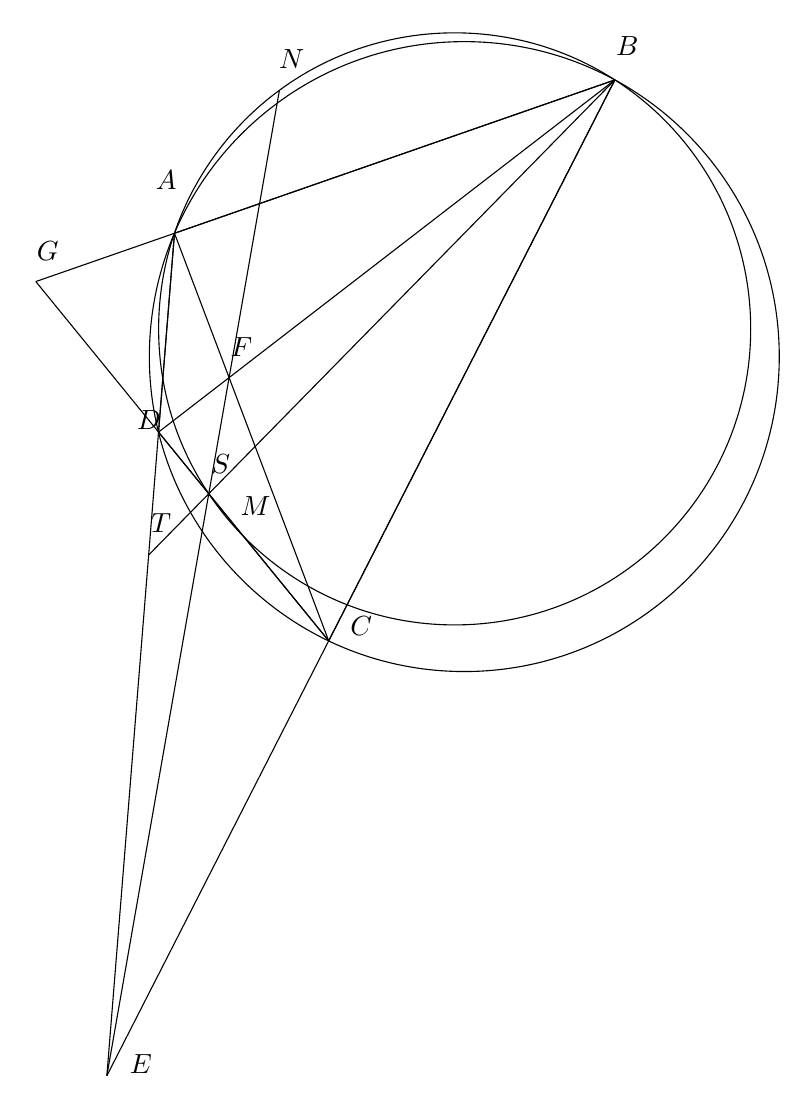
\begin{tikzpicture}
	\draw (-1,2) circle [radius = 4];
\draw (-4.680695002545015,3.5660409631424574)-- (0.9119008964936051,5.513493270519662);
\draw (0.9119008964936051,5.513493270519662)-- (-2.722209881497651,-1.6102621960284056);
\draw (-2.722209881497651,-1.6102621960284056)-- (-4.883378203882584,1.041160219009623);
\draw (-4.883378203882584,1.041160219009623)-- (-4.680695002545015,3.5660409631424574);
\draw (-4.680695002545015,3.5660409631424574)-- (-2.722209881497651,-1.6102621960284056);
\draw (-1.1225373688096725,2.351896672225524) circle [radius = 3.759605312486309];
\draw (-4.883378203882584,1.041160219009623)-- (0.9119008964936051,5.513493270519662);
\draw (-4.680695002545015,3.5660409631424574)-- (-5.539549217436753,-7.132943732613465);
\draw (-5.539549217436753,-7.132943732613465)-- (0.9119008964936051,5.513493270519662);
\draw (0.9119008964936051,5.513493270519662)-- (-6.441599652336171,2.9528591983207706);
\draw (-6.441599652336171,2.9528591983207706)-- (-2.722209881497651,-1.6102621960284056);
\draw (-5.539549217436753,-7.132943732613465)-- (-3.348102884842708,5.381994069920833);
\draw (-5.008663323011488,-0.5195511903592608)-- (0.9119008964936051,5.513493270519662);
\draw (-4.53,4) node [above left] {$A$};
\draw (1.07,5.94) node {$B$};
\draw (-2.57,-1.18) node [below right] {$C$};
\draw (-4.73,1.44) node [below left] {$D$};
\draw (-5.37,-6.74) node [below right] {$E$};
\draw (-3.83,2.12) node {$F$};
\draw (-3.65,0.1) node {$M$};
\draw (-3.19,5.78) node {$N$};
\draw (-6.29,3.34) node {$G$};
\draw (-4.09,0.64) node {$S$};
\draw (-4.85,-0.12) node {$T$};
\end{tikzpicture}
\end{center}
\textbf{Lời giải.} Gọi \(G\) là giao điểm của \(AB\) và \(CD\), \(S\) là giao điểm của \(EF\) và \(CD\).\\
Ta có: \(\left( {GSDC} \right) =  - 1\) (hàng điều hòa tứ giác toàn phần).\\
\(M\) là trung điểm của \(CD\) nên theo công thức Maclaurin, ta có: \(\overline {GS} .\overline {GM}  = \overline {GD} .\overline {GC} \)\\
Mà \(\overline {GD} .\overline {GC}  = \overline {GA} .\overline {GB} \) (phương tích của điểm \(G\) đến đường tròn \(\left( O \right)\)).\\
\( \Rightarrow \overline {GS} .\overline {GM}  = \overline {GA} .\overline {GB} \) \( \Rightarrow \) \(A, B, M, S\) cùng thuộc một đường tròn. \\
Gọi \(T\) là giao điểm của \(SB\) và \(DE\).\\
\( \Rightarrow \left( {TADE} \right) =  - 1\) (hàng điều hòa tứ giác toàn phần \(DECF\).\\
\( \Rightarrow S\left( {TADE} \right) =  - 1 \Rightarrow S\left( {BANM} \right) =  - 1.\)\\
Do đó, tứ giác \(BNAM\) là tứ giác điều hòa.\\
\newline
\textbf{Ví dụ 3.} Cho tam giác \(ABC\) nội tiếp đường tròn \(\left( O \right)\), ngoại tiếp đường tròn \(\left( I \right)\). Gọi \(M\) là tiếp điểm của \(BC\) với \(\left( I \right)\), \(D\) là giao điểm thứ hai của \(AM\) và \(\left( O \right)\). Chứng minh rằng nếu \(OI\) vuông góc với \(AM\) thì tứ giác \(ABDC\) là tứ giác điều hòa. (Đề kiểm tra chọn đội tuyển Ninh Bình)
\begin{center}
	\begin{tikzpicture}
	\draw (4,2) circle [radius = 4];
\draw (1.974549266863309,5.449282436628819)-- (0.12801240733679675,0.9961513648650955);
\draw (0.12801240733679675,0.9961513648650955)-- (6.59794340049406,-1.0414947127735337);
\draw (6.59794340049406,-1.0414947127735337)-- (1.974549266863309,5.449282436628819);
\draw (2.361472246403431,2.037554988178855) circle [radius = 1.6642270529445828];
\draw (1.974549266863309,5.449282436628819)-- (1.8207576777622225,-1.354236560078567);
\draw (4,2)-- (1.8976684459856412,2.0481853520550635);
\draw (-3.607037434561864,2.1724714319846425)-- (3.7169800706157816,3.0030860452928727);
\draw (-3.607037434561864,2.1724714319846425)-- (6.59794340049406,-1.0414947127735337);
\draw (0.12801240733679675,0.9961513648650955)-- (1.7335204787977654,-5.196522625055785);
\draw (1.7335204787977654,-5.196522625055785)-- (6.59794340049406,-1.0414947127735337);
\draw (4.16,2.43) node {$O$};
\draw (2.14,5.87) node {$A$};
\draw (0.52,1.43) node {$B$};
\draw (6.9,-0.65) node {$C$};
\draw (2.52,2.43) node {$I$};
\draw (2.02,0.85) node {$M$};
\draw (1.98,-0.97) node {$D$};
\draw (3.52,0.37) node {$N$};
\draw (2.06,2.43) node {$P$};
\draw (3.88,3.39) node {$E$};
\draw (1.1,2.99) node {$F$};
\draw (-3.44,2.57) node {$S$};
\draw (1.82,-4.49) node {$Q$};
	\end{tikzpicture}
\end{center}
\textbf{Lời giải.} Gọi \(N\) là trung điểm \(BC\); \(E, F\) lần lượt là tiếp điểm của đường tròn \(\left( I \right)\) với \(AC, AB\).\\
Gọi \(S\) là giao điểm của \(EF\) và \(BC\), \(P\) là giao điểm của \(OI\) và \(AM\). \\
\( \Rightarrow \) \(A, F, P, I, E\) cùng thuộc đường tròn đường kính \(AI\).\\
Ta có: \({P_{S/\left( {IM} \right)}} = S{M^2} = \overline {SF} .\overline {SE}  = {P_{S/\left( {IA} \right)}}\) với \(P\) là kí hiệu phương tích từ một điểm đến một đường tròn.\\
\( \Rightarrow \) \(S\) là điểm đẳng phương của đường tròn đường kính \(IM\) và đường tròn đường kính \(AI\).\\
Mà hai đường tròn này cắt nhau tại \(I\) và \(P\) nên \(S, P, I, O\) thẳng hàng.\\
Ta có \(\left( {SMBC} \right) =  - 1\) (hàng điều hòa tứ giác toàn phần \(EFBC\)).\\
\( \Rightarrow \overline {SB} .\overline {SC}  = \overline {SM} .\overline {SN} \) (Maclaurin).\\
\(\overline {SP} .\overline {SO}  = \overline {SM} .\overline {SN} \) (\(M, P, O, N\) đồng viên).
\( \Rightarrow \overline {SB} .\overline {SC}  = \overline {SP} .\overline {SO} \)\\
\( \Rightarrow \) \(B, P, O, C\) đồng viên.\\
Gọi \(Q\) là giao điểm của hai tiếp tuyến tại \(B\) và \(C\) của đường tròn \(\left( O \right)\).\\
\( \Rightarrow \) \(B, P, O, C, Q\) cùng thuộc đường tròn đường kính \(OQ\).\\
\( \Rightarrow \widehat {OPQ} = {90^ \circ }\), mà theo giả thiết ta được \(\widehat {OPQ} = {90^ \circ }\) nên \(A, P, D, Q\) thẳng hàng \( \Rightarrow \) \(BQ, CQ, AD\) đồng quy tại \(Q\).\\
\( \Rightarrow \) Tứ giác \(ABCD\) là tứ giác điều hòa.
\newpage
\textbf{Ví dụ 4.} Cho hình bình hành \(ABCD\), \(M\) là một điểm nằm trên đường chéo \(BD\). \(AM\) cắt \(CD, CB\) lần lượt tại \(K, N\). Gọi \(\left( {{C_1}} \right)\) là đường tròn tâm \(M\), bán kính \(MA\); \(\left( {{C_2}} \right)\) là đường tròn ngoại tiếp tam giác \(KCN\). \(\left( {{C_1}} \right)\) và \(\left( {{C_2}} \right)\) cắt nhau tại \(P, Q\). Chứng minh rằng tứ giác \(PKQN\) là tứ giác điều hòa. (A. Rermerov)\\
\begin{center}
	\begin{tikzpicture}
	\draw (-4,3)--(2,3);
\draw (2,3)--(-1,1);
\draw (-1,1)--(-7,1);
\draw (-7,1)--(-4,3);
\draw (-7,1)--(2,3);
\draw (-1.243176470588235,2.279294117647059) circle [radius=2.8494723969844786];
\draw (1.3251714005876594,-1.068684082672917) circle [radius=3.112213983005517];
\draw (-4,3)--(3.650342801175319,1);
\draw (3.650342801175319,1)--(-1,1);
\draw (-4,3)--(-1,1);
\draw (-3.83,3.42) node {$A$};
\draw (2.17,3.42) node {$B$};
\draw (-1.05,1.44) node {$C$};
\draw (-6.83,1.42) node {$D$};
\draw (-1.09,2.7) node {$M$};
\draw (3.81,1.38) node {$K$};
\draw (0.87,2.16) node {$N$};
\draw (1.75,2.42) node {$P$};
\draw (-1.57,-0.14) node {$Q$};
\draw (-2.33,2.38) node {$O$};
\draw (1.67,1.94) node [below] {$E$};
	\end{tikzpicture}
\end{center}
\textbf{Lời giải.} Gọi \(O\) là trung điểm \(AC\), \(E\) là giao điểm thứ hai của \(AM\) và \(\left( {{C_1}} \right)\).\\
\(MO\) là đường trung bình của tam giác \(CAE\) nên \(CE\) song song với \(BD\).
\( \Rightarrow C\left( {EDOB} \right) =  - 1\) (chùm điều hòa trung tuyến).\\
Hay \(\left( {AEKN} \right) =  - 1.\) \\
\( \Rightarrow M{A^2} = \overline {MK} .\overline {MN} \) (Newton). Lại có \(P, Q\) cùng thuộc đường tròn \(\left( {{C_1}} \right)\) nên \(MA = MP = MQ\) \( \Rightarrow \overline {MK} .\overline {MN}  = M{P^2} = M{Q^2}.\)
\( \Rightarrow \) \(MP, MQ\) là tiếp tuyến của \(\left( {{C_2}} \right)\), do đó tứ giác \(PKQN\) là tứ giác điều hòa.\\
\newpage
\textbf{Ví dụ 5.} Cho tam giác \(ABC\) không cân, \(M\) là trung điểm \(BC\). Đường tròn đường kính \(AM\) lần lượt cắt \(AB, AC, BC\) tại điểm thứ hai \(P, Q, R\). Tiếp tuyến tại \(P, Q\) của đường tròn đường kính \(AM\) cắt nhau tại \(S\). Chứng minh rằng \(SB = SC\).\\
\begin{center}
	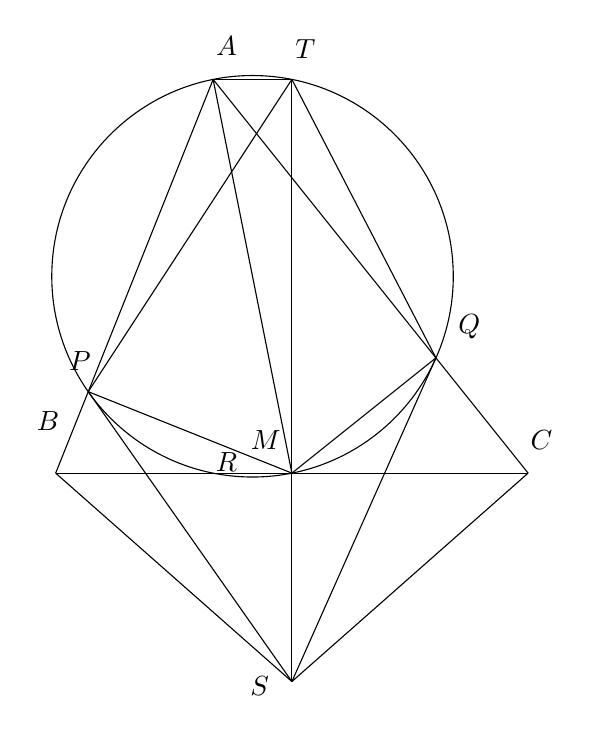
\begin{tikzpicture}
	\draw (-2,4)--(-4,-1);
\draw (-4,-1)--(2,-1);
\draw (2,-1)--(-2,4);
\draw (-2,4)--(-1,-1);
\draw (-1.5,1.5) circle [radius=2.5495097567963922];
\draw (-4,-1)--(-1,-3.6470588235294117);
\draw (-1,-3.6470588235294117)--(2,-1);
\draw (-1,4)--(-1,-3.6470588235294117);
\draw (-1,-3.6470588235294117)--(-3.586206896551724,0.034482758620689884);
\draw (-1,-3.6470588235294117)--(0.8292682926829267,0.46341463414634165);
\draw (-1,4)--(0.8292682926829267,0.46341463414634165);
\draw (0.8292682926829267,0.46341463414634165)--(-1,-1);
\draw (-1,-1)--(-3.586206896551724,0.034482758620689884);
\draw (-3.586206896551724,0.034482758620689884)--(-1,4);
\draw (-2,4)--(-1,4);
\draw (-1.83,4.42) node {$A$};
\draw (-3.83,-0.58) node [above left] {$B$};
\draw (2.17,-0.58) node {$C$};
\draw (-1.33,-0.58) node {$M$};
\draw (-3.43,0.42) node [left] {$P$};
\draw (0.99,0.86) node [right] {$Q$};
\draw (-1.83,-0.62) node [below] {$R$};
\draw (-1.41,-3.46) node [below] {$S$};
\draw (-0.83,4.38) node {$T$};
	\end{tikzpicture}
\end{center}
\textbf{Lời giải.} Gọi \(T\) là giao điểm thứ hai của \(SM\) với đường tròn đường kính \(AM\). Khi đó, ta có tứ giác \(TPMQ\) là tứ giác điều hòa.\\
Điểm \(A\) nằm trên đường tròn ngoại tiếp tứ giác \(TPMQ\) nên \(A\left( {TMPQ} \right) =  - 1.\)\\
\( \Rightarrow A\left( {TMBC} \right) =  - 1\).
Mà \(M\) là trung điểm \(BC\) nên chùm \(A\left( {TMBC} \right)\) là chùm trung tuyến, do đó \(AT\) song song với \(BC\).\\
Lại có \(AT \bot TM\) hay \(AT \bot SM\) (do \(T\) thuộc đường tròn đường kính \(AM\)).\\
\( \Rightarrow SM \bot BC\) tại trung điểm \(M\) của \(BC\) nên \(SM\) là đường trung trực của \(BC\).\\
Vậy \(SB = SC\).\\
\textbf{Nhận xét:} Bài toán trên là một bài toán khá đơn giản, ta hoàn toàn có thể nhìn ra điểm \(T\) một cách dễ dàng. Dù vậy, kết luận của bài toán này thực sự rất thú vị, nó xuất hiện trong nhiều bài toán khác như sau:\\
\textbf{Ví dụ 5.1.} Cho tam giác \(ABC\) có \(M, N, P\) lần lượt là trung điểm của \(AB, AC, BC\). Kẻ \(BI\) vuông góc với \(MP\) tại \(I\), \(CK\) vuông góc với \(NP\) tại \(K\). Tiếp tuyến tại \(I, K\) của đường tròn ngoại tiếp tam giác \(IKP\) cắt nhau tại \(T\). Chứng minh rằng \(TB = TC\). (VMO 2014).\\
\textbf{Ví dụ 5.2.} Cho tứ giác \(ABCD\) nội tiếp đường tròn \(\left( O \right)\). Kẻ \(OM\) vuông góc với \(AD\) \(\left( {M \in AC} \right)\), \(ON\) vuông góc với \(BC\) \(\left( {N \in BD} \right).\) Tiếp tuyến tại \(M\) và \(N\) của đường tròn ngoại tiếp tam giác \(OMN\) cắt nhau tại \(S\). Chứng minh rằng \(SB = SC\).\\
\newpage
\textbf{Ví dụ 6.} Cho tam giác \(ABC\), \(M, N\) lần lượt nằm trên \(AB, AC\) sao cho \(MN\) song song với \(BC\). Gọi \(P\) là giao điểm của \(CM\) và \(BN\). Đường tròn ngoại tiếp hai tam giác \(MBP\) và \(NPC\) cắt nhau tại điểm thứ hai \(Q\)) . Chứng minh rằng \(\widehat {BAQ} = \widehat {PAC}.\)
\begin{center}
	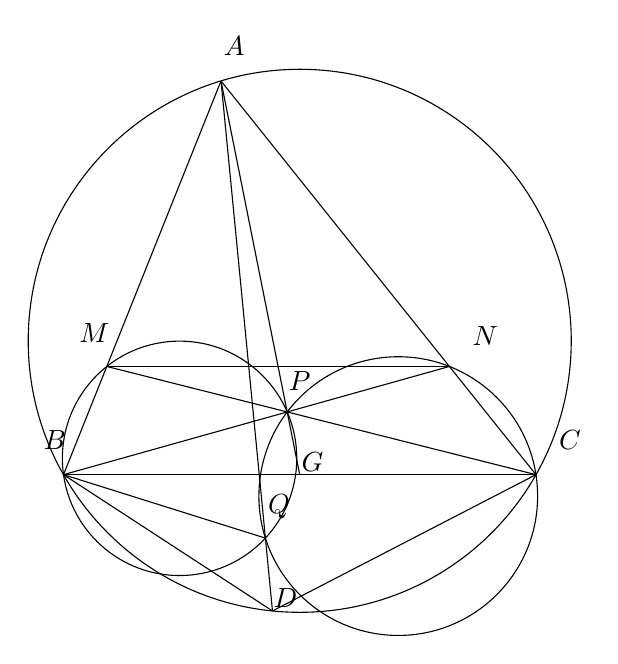
\begin{tikzpicture}
	\draw (-2,4)--(-4,-1);
\draw (-4,-1)--(2,-1);
\draw (2,-1)--(-2,4);
\draw (-4,-1)--(0.900689655172414,0.37413793103448256);
\draw (2,-1)--(-3.450344827586207,0.37413793103448256);
\draw (-2.526152475181558,-0.7925390099273772) circle [radius=1.4883771661831426];
\draw (0.2513248889746612,-1.2721469853719953) circle [radius=1.769725579169422];
\draw (-2,4)--(-1.4360013262599467,-1.8058687002652523);
\draw (-2,4)--(-1,-1);
\draw (-1,0.7) circle [radius=3.448187929913333];
\draw (-4,-1)--(-1.3461538461538458,-2.73076923076923);
\draw (-1.3461538461538458,-2.73076923076923)--(2,-1);
\draw (-4,-1)--(-1.4360013262599467,-1.8058687002652523);
\draw (-1.4360013262599467,-1.8058687002652523)--(-1.3461538461538458,-2.73076923076923);
\draw (-3.450344827586207,0.37413793103448256)--(0.900689655172414,0.37413793103448256);
\draw (-1.8323330471083827,4.439526375162066) node {$A$};
\draw (-3.843592286411753,-0.5581480982584288) node [left] {$B$};
\draw(2.1698696816064054,-0.5581480982584288) node [right] {$C$};
\draw (-3.2950670393290156,0.8030071445024376) node [left] {$M$};
\draw (1.0728191874409303,0.7623756447185313) node [right] {$N$};
\draw (-0.9993873015382999,0.19353464774384077) node {$P$};
\draw (-1.263492050133692,-1.4114095937204645) node {$Q$};
\draw (-0.836861302402674,-0.5987795980423352) node [below] {$G$};
\draw (-1.182229050565879,-2.32561833885836) node [below] {$D$};
	\end{tikzpicture}
\end{center}
\textbf{Lời giải.} Gọi \(G\) là giao điểm của \(AP\) và \(BC\), \(AQ\) cắt đường tròn \(\left( {ABC} \right)\) tại điểm thứ hai \(D\).\\
Theo định lí Ceva, ta được \(G\) là trung điểm của \(BC\).\\
Xét mod \(\pi \): \(\left( {BQ,BM} \right) \equiv \left( {PQ,PC} \right) \equiv \left( {NQ,NC} \right).\)\\
\(\Rightarrow\) \(B, A, N, Q\) đồng viên \( \Rightarrow \widehat {BQD} = \widehat {BNC}.\)\\
\(\Rightarrow\) Hai tam giác \(BQD\) và \(BNC\) đồng dạng \( \Rightarrow \frac{{BD}}{{BC}} = \frac{{QD}}{{NC}}.\)\\
Tương tự: \(\frac{{CD}}{{BC}} = \frac{{QD}}{{MB}}\). Khi đó: \(\frac{{BD}}{{CD}} = \frac{{MB}}{{NC}} = \frac{{AB}}{{AC}}.\)\\
Do đó, tứ giác \(ABDC\) là tứ giác điều hòa. \\
\(G\) là trung điểm \(BC\) nên \(\widehat {BAD} = \widehat {GAC}\), suy ra đpcm.\\
\textbf{Nhận xét:} Đây là một bài toán hay và lạ. Bài toán không hề nhắc đến tứ giác điều hòa hay các tính chất của nó, tuy vậy ta vẫn có thể nhìn ra \(G\) là trung điểm \(BC\) cộng với yêu cầu của đề bài để tìm cách chứng minh \(AQ\) là đường đối trung của tam giác \(ABC\), hay \(ABCD\) là tứ giác điều hòa. Sau đây xin gửi đến bạn đọc một bài toán tương tự, cũng khá hay và đẹp:
\textbf{Ví dụ 6.1.} Cho tam giác \(ABC\) nội tiếp đường tròn \(\left( O \right)\) và một điểm \(P\) nằm bên trong tam giác. \(AP, BP, CP\) lần lượt cắt \(BC, CA, AB\) tại \(D, E, F\). Tiếp tuyến tại \(A\) của đường tròn \(\left( O \right)\), \(EF, BC\) đồng quy tại \(S\). Đường tròn ngoại tiếp tam giác \(SAD\) cắt đường tròn \(\left( O \right)\) tại điểm thứ hai \(G\). \(GE, GF\) lần lượt cắt \(\left( O \right)\) tại điểm thứ hai \(M, N\). \(CN\) cắt \(DM\) tại \(I\). Chứng minh rằng \(\widehat {ABD} = \widehat {IAC}\).
\newpage
\textbf{Ví dụ 7.} Cho đường tròn \(\left( O \right)\) đường kính \(AB\). Trên tiếp tuyến tại \(A\) của \(\left( O \right)\), lấy điểm \(M\) khác \(A\). Từ \(M\), kẻ cát tuyến \(MCD\) đến đường tròn \(\left( O \right)\). \(MO\) cắt \(BC, BD\) lần lượt tại \(X, Y\). Chứng minh rằng \(OX = OY\).
\begin{center}
	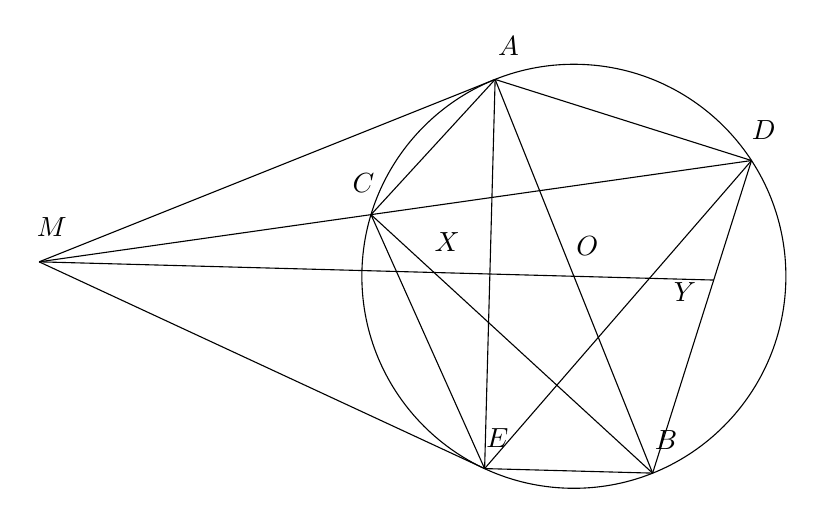
\begin{tikzpicture}
	\draw (-3,4)--(-1,-1);
\draw (-2,1.5) circle [radius=2.692582403567252];
\draw (-8.791379310344828,1.6834482758620686)--(-3,4);
\draw (-8.791379310344828,1.6834482758620686)--(0.2560911391146048,2.9697117989621518);
\draw (-1,-1)--(-4.5763123049252155,2.282697200385263);
\draw (-1,-1)--(0.2560911391146048,2.9697117989621518);
\draw (-8.791379310344828,1.6834482758620686)--(-0.22413168226454203,1.4520303658271);
\draw (-8.791379310344828,1.6834482758620686)--(-3.1335029611783183,-0.9423699631710146);
\draw (-3,4)--(-4.5763123049252155,2.282697200385263);
\draw (-4.5763123049252155,2.282697200385263)--(-3.1335029611783183,-0.9423699631710146);
\draw (-3.1335029611783183,-0.9423699631710146)--(0.2560911391146048,2.9697117989621518);
\draw (0.2560911391146048,2.9697117989621518)--(-3,4);
\draw (-3.1335029611783183,-0.9423699631710146)--(-1,-1);
\draw (-3,4)--(-3.1335029611783183,-0.9423699631710146);
\draw (-2.83,4.42) node {$A$};
\draw (-0.83,-0.58) node {$B$};
\draw (-1.83,1.88) node {$O$};
\draw (-8.63,2.12) node {$M$};
\draw (-4.41,2.68) node [left] {$C$};
\draw (0.41,3.36) node {$D$};
\draw (-3.61,1.94) node {$X$};
\draw (-0.59,1.3) node {$Y$};
\draw (-2.97,-0.56) node {$E$};
	\end{tikzpicture}
\end{center}
\textbf{Lời giải.} Gọi \(ME\) là tiếp tuyến thứ hai từ \(M\) đến \(\left( O \right)\) (\(E\) là tiếp điểm).\\
Ta được tứ giác \(ACED\) là tứ giác điều hòa.\\
\( \Rightarrow B\left( {AECD} \right) =  - 1\) hay \(B\left( {OEXY} \right) =  - 1.\)\\
Mà \(MO\) song song với \(BE\) do cùng vuông góc với \(AE\) nên \(OX = OY\) (chùm điều hòa trung tuyến).\\
\textbf{Nhận xét:} Thực sự rất ấn tượng với lời giải ngắn gọn bằng tứ giác điều hòa của bài toán. Nếu giải bằng kiến thức Trung học Cơ sở, ta sẽ phải xét hai trường hợp với lời giải khá rắc rối cùng hình phụ. Bài toán trên đồng thời cũng là một bổ đề hay được sử dụng nhiều trong các kết quả đẹp khác, chẳng hạn như:\\
\textbf{Ví dụ 7.1.} Từ một điểm \(M\) ở ngoài đường tròn \(\left( O \right)\), kẻ tiếp tuyến \(MA\), cát tuyến \(MBC\) đến đường tròn. \(D, E\) lần lượt là điểm đối xứng với \(C, A\) qua \(O\). .Chứng minh rằng \(EB, DA, MO\) đồng quy.
\begin{center}
	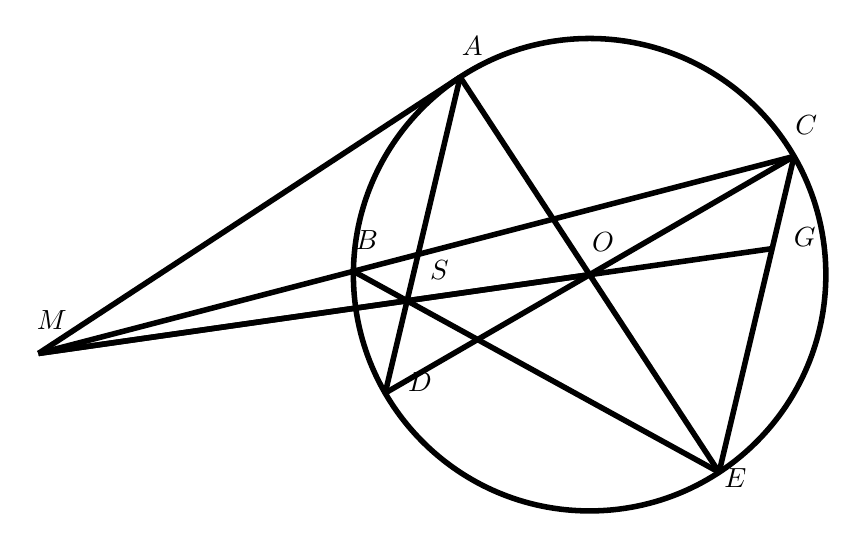
\begin{tikzpicture}
	\draw [line width=2pt] (-2,2) circle (3cm);
\draw [line width=2pt] (-0.3558125457540289,-0.5093121797217961)-- (-4.999685525956368,2.0434366822843026);
\draw [line width=2pt] (-4.596293069310363,0.49691573814008283)-- (-3.644187454245971,4.509312179721796);
\draw [line width=2pt] (-9,1)-- (-2,2);
\draw [line width=2pt] (-9,1)-- (-3.644187454245971,4.509312179721796);
\draw [line width=2pt] (-9,1)-- (0.5962930693103634,3.503084261859917);
\draw [line width=2pt] (0.5962930693103634,3.503084261859917)-- (-0.3558125457540289,-0.5093121797217961);
\draw [line width=2pt] (-3.644187454245971,4.509312179721796)-- (-0.3558125457540289,-0.5093121797217961);
\draw [line width=2pt] (-4.596293069310363,0.49691573814008283)-- (0.5962930693103634,3.503084261859917);
\draw [line width=2pt] (-9,1)-- (0.31820899106312506,2.331172713009018);
\draw (-1.83,2.42) node {$O$};
\draw (-8.83,1.42) node {$M$};
\draw (-3.49,4.9) node {$A$};
\draw (-4.83,2.44) node {$B$};
\draw (0.75,3.9) node {$C$};
\draw (-4.43,0.88) node [below right] {$D$};
\draw (-0.15,-0.58) node {$E$};
\draw (0.47,2.72) node [ below right] {$G$};
\draw (-4.15,2.06) node [right] {$S$};
	\end{tikzpicture}
\end{center}
\textbf{Gợi ý.} Gọi \(G, S\) lần lượt là giao điểm của \(MO\) với \(EC, EB\).\\
Theo ví dụ 7, ta có \(O\) là trung điểm \(GS\) \( \Rightarrow \) \(DS\) song song với \(EC\).\\
Mà tứ giác \(DACE\) là hình chữ nhật nên \(DA\) song song với \(CE\). Do đó, \(D, S, A\) thẳng hàng.\\
\textbf{Ví dụ 7.2} Cho tam giác \(ABC\) nội tiếp đường tròn \(\left( O \right)\) có phân giác \(AD\). Dây cung \(PQ\) bất kì của \(\left( O \right)\) song song với \(BC\). \(PD, QD\) lần lượt cắt \(\left( O \right)\) tại điểm thứ hai \(X, Y\). \(G\) là điểm đối xứng với \(A\) qua \(O\). \(XY\) cắt \(BC\) tại \(M\), \(GX\) cắt \(MO\) tại \(H\), \(GY\) cắt \(MO\) tại \(K\). Chứng minh rằng \(O\) là trung điểm của \(HK\).
\begin{center}
	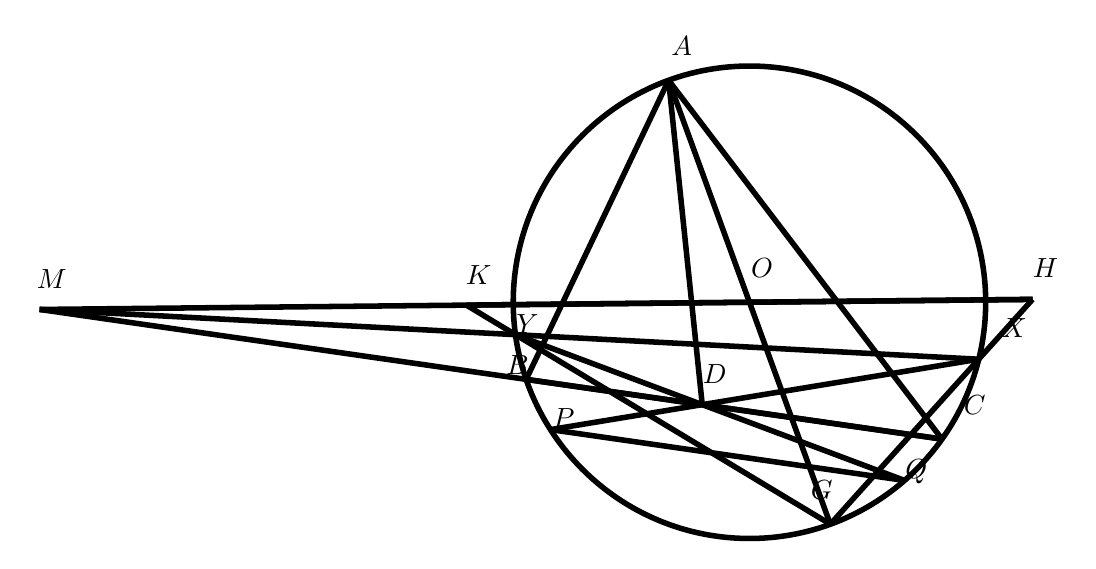
\begin{tikzpicture}
	\draw [line width=2pt] (-2,2) circle (3cm);
\draw [line width=2pt] (-3.026845637583893,4.818791946308725)-- (-4.835685071828252,1.0207706226780144);
\draw [line width=2pt] (-4.835685071828252,1.0207706226780144)-- (0.44529009790873797,0.26202521966817005);
\draw [line width=2pt] (0.44529009790873797,0.26202521966817005)-- (-3.026845637583893,4.818791946308725);
\draw [line width=2pt] (-3.026845637583893,4.818791946308725)-- (-0.973154362416107,-0.8187919463087248);
\draw [line width=2pt] (-5.594965952707814,1.9635744954663605)-- (1.5949659527078155,2.036425504533639);
\draw [line width=2pt] (-4.526814201984534,0.3828389107298984)-- (-0.030689428310152197,-0.2631429190907508);
\draw [line width=2pt] (-4.526814201984534,0.3828389107298984)-- (0.9114507016762089,1.2764982296434162);
\draw [line width=2pt] (-0.030689428310152197,-0.2631429190907508)-- (-4.971618230678742,1.5883143297396205);
\draw [line width=2pt] (0.9114507016762089,1.2764982296434162)-- (-11.01546503124018,1.9086520243339298);
\draw [line width=2pt] (-11.01546503124018,1.9086520243339298)-- (0.44529009790873797,0.26202521966817005);
\draw [line width=2pt] (-0.973154362416107,-0.8187919463087248)-- (1.5949659527078155,2.036425504533639);
\draw [line width=2pt] (-0.973154362416107,-0.8187919463087248)-- (-5.594965952707814,1.9635744954663605);
\draw [line width=2pt] (-11.01546503124018,1.9086520243339298)-- (1.5949659527078155,2.036425504533639);
\draw [line width=2pt] (-3.026845637583893,4.818791946308725)-- (-2.5997092798627697,0.6995162522508952);
\draw (-1.84,2.43) node {$O$};
\draw (-2.86,5.25) node {$A$};
\draw (-4.68,1.45) node [below left] {$B$};
\draw (0.6,0.69) node [right] {$C$};
\draw (-2.44,1.09) node {$D$};
\draw (-4.36,0.77) node [below] {$P$};
\draw (0.12,0.13) node [below] {$Q$};
\draw (1.08,1.67) node [right] {$X$};
\draw (-4.82,1.97) node [below] {$Y$};
\draw (-0.82,-0.39) node [left] {$G$};
\draw(-10.86,2.29) node {$M$};
\draw (1.76,2.43) node {$H$};
\draw (-5.44,2.35) node {$K$};
	\end{tikzpicture}
\end{center}
\textbf{Gợi ý.} Tiếp tuyến tại \(A\) của đường tròn \(\left( O \right)\) cắt \(BC\) tại \(M'\).\\
Ta có: \(A{{M'}^2} = \overline {M'B} .\overline {M'C} \), mà \(AM' = DM'\) nên \(D{{M'}^2} = \overline {M'B} .\overline {M'C} \).\\
Lại có hai tam giác \(MDY\) và \(MXD\) đồng dạng nên \(M{D^2} = \overline {MX} .\overline {MY}  = \overline {MB} .\overline {MC} \).\\
Vậy \(M' \equiv M\), dẫn đến đpcm.\\
\textbf{Nhận xét:} Hai bài toán trên nếu không biết cách đưa về bổ đề quen thuộc thì sẽ dẫn đến thế khó, cả hai bài đều có sự phức tạp về hình vẽ, khó suy đoán hướng làm, thế nhưng nếu biết cách tận dụng yếu tố tứ giác điều hòa để giải quyết thì vấn đề sẽ trở nên đơn giản.\\
\newline
\textbf{Ví dụ 8.} Cho tứ giác \(ABCD\) nội tiếp đường tròn \(\left( O \right)\), \(AC\) cắt \(BD\) tại \(M\). Đường thẳng qua \(M\) và vuông góc với \(MO\) cắt \(BC\) tại \(P\), \(DP\) cắt \(\left( O \right)\) tại điểm thứ hai \(S\). Lấy điểm \(Q\) nằm trên \(\left( O \right)\) sao cho \(DQ\) vuông góc với \(OM\). TIa phân giác các góc \(\widehat {ABS},\widehat {AQS}\) cắt nhau tại \(R\). Tiếp tuyến tại \(B, Q\) của \(\left( O \right)\) cắt nhau tại \(T\). Chứng minh rằng \(A, R, S, T\) thẳng hàng.\\
\textbf{Lời giải.}
\textbf{Bổ đề:} Cho đường tròn \(\left( O \right)\) với dây cung \(AB\). Gọi \(I\) là trung điểm của \(AB\), qua \(I\) dựng hai dây cung \(MN, PQ\) sao cho \(MP, NQ\) cắt \(AB\) lần lượt tại \(E, F\). Chứng minh rằng \(I\) là trung điểm của \(EF\).
\begin{center}
	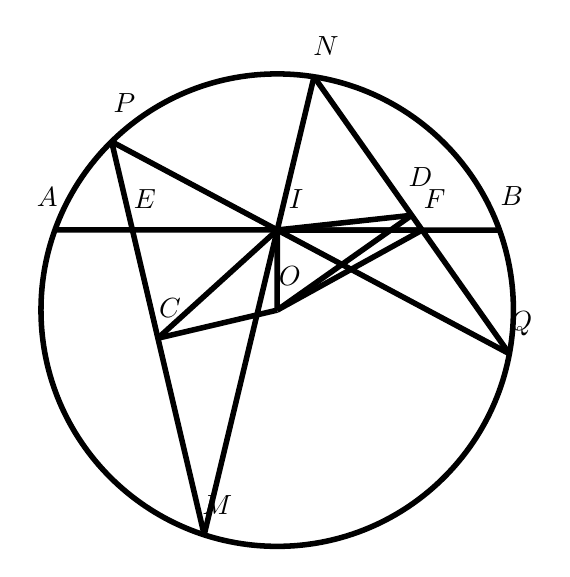
\begin{tikzpicture}
	\draw [line width=2pt] (4,2) circle (3cm);
\draw [line width=2pt] (1.178871322748484,3.0204082449633143)-- (6.8229210378474665,3.01543922224729);
\draw [line width=2pt] (4,2)-- (2.4850001842945133,1.6433182311625663);
\draw [line width=2pt] (4,2)-- (5.707887943958493,3.204729528997322);
\draw [line width=2pt] (4.000896180297975,3.0179237336053024)-- (4,2);
\draw [line width=2pt] (4.000896180297975,3.0179237336053024)-- (5.84080178285569,3.0163038802737496);
\draw [line width=2pt] (4.000896180297975,3.0179237336053024)-- (5.707887943958493,3.204729528997322);
\draw [line width=2pt] (4,2)-- (5.84080178285569,3.0163038802737496);
\draw [line width=2pt] (4.000896180297975,3.0179237336053024)-- (2.4850001842945133,1.6433182311625663);
\draw [line width=2pt] (1.8972591262035121,4.139738492822332)-- (3.072741242385514,-0.853102030497199);
\draw [line width=2pt] (3.072741242385514,-0.853102030497199)-- (4.467356044850927,4.963372795876566);
\draw [line width=2pt] (4.467356044850927,4.963372795876566)-- (6.948419843066058,1.4460862621180781);
\draw [line width=2pt] (6.948419843066058,1.4460862621180781)-- (1.8972591262035121,4.139738492822332);
\draw (4.16,2.43) node {$O$};
\draw (1.08,3.43) node {$A$};
\draw (6.98,3.45) node {$B$};
\draw (4.24,3.41) node {$I$};
\draw (3.24,-0.47) node {$M$};
\draw (4.62,5.35) node {$N$};
\draw (2.06,4.63) node {$P$};
\draw (7.1,1.83) node {$Q$};
\draw (2.32,3.41) node {$E$};
\draw (6,3.41) node {$F$};
\draw (2.64,2.03) node {$C$};
\draw (5.82,3.69) node {$D$};
	\end{tikzpicture}
\end{center}
Vì \(I\) là trung điểm của \(AB\) nên \(OI \bot AB.\)\\
Gọi \(C, D\) lần lượt là trung điểm của \(MP, NQ\) \( \Rightarrow OC \bot MP\) và \(OD \bot NQ\).\\
Vậy các tứ giác \(IOCE, IODF\) là tứ giác nội tiếp.\\
\( \Rightarrow \widehat {IOE} = \widehat {ICE}\) và \(\widehat {IOF} = \widehat {IDF}\).\\
Mặt khác, hai tam giác \(IMP\) và \(IQN\) đồng dạng và \(IC, ID\) là hai đường trung tuyến tương ứng \( \Rightarrow \frac{{IC}}{{ID}} = \frac{{IP}}{{IN}} = \frac{{PM}}{{NQ}} = \frac{{CP}}{{DN}}.\) Do đó, hai tam giác \(ICP\) và \(IDN\) đồng dạng. Từ đó, ta có: \(\widehat {ICE} = \widehat {IDF}.\) \\
Do đó: \(\widehat {IOE} = \widehat {IOF}\) \( \Rightarrow \) tam giác \(OEF\) cân tại \(O\) \( \Rightarrow \) \(I\) là trung điểm \(EF\).\\
\textbf{Quay lại bài toán:} 
\begin{center}
	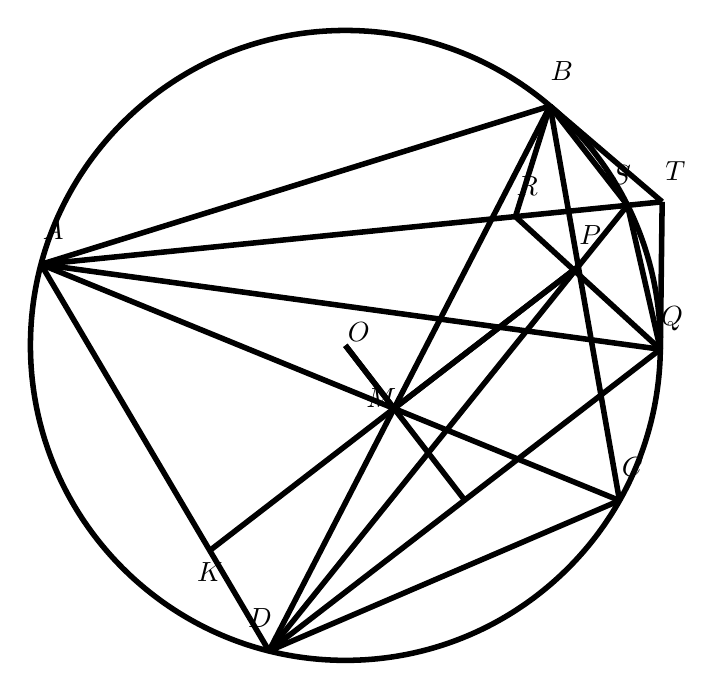
\begin{tikzpicture}
	\draw [line width=2pt] (-2,2) circle (4cm);
\draw [line width=2pt] (-5.865436646601809,3.0287854640826524)-- (0.599031079596668,5.040565317057106);
\draw [line width=2pt] (0.599031079596668,5.040565317057106)-- (1.4811099882756102,0.029752997838144335);
\draw [line width=2pt] (1.4811099882756102,0.029752997838144335)-- (-2.970142500145332,-1.8805700005813275);
\draw [line width=2pt] (-2.970142500145332,-1.8805700005813275)-- (-5.865436646601809,3.0287854640826524);
\draw [line width=2pt] (-5.865436646601809,3.0287854640826524)-- (1.4811099882756102,0.029752997838144335);
\draw [line width=2pt] (-2.970142500145332,-1.8805700005813275)-- (0.599031079596668,5.040565317057106);
\draw [line width=2pt] (-2,2)-- (-1.3822226566946776,1.1986324715157703);
\draw [line width=2pt] (-1.3822226566946776,1.1986324715157703)-- (0.9577918005317896,3.002558714217107);
\draw [line width=2pt] (-2.970142500145332,-1.8805700005813275)-- (1.5825172888326289,3.7792048435228898);
\draw [line width=2pt] (-2,2)-- (-0.4852231741740759,0.035063968803776255);
\draw [line width=2pt] (-2.970142500145332,-1.8805700005813275)-- (1.9996961517971803,1.95069793818888);
\draw [line width=2pt] (0.599031079596668,5.040565317057106)-- (1.5825172888326289,3.7792048435228898);
\draw [line width=2pt] (1.5825172888326289,3.7792048435228898)-- (1.9996961517971803,1.95069793818888);
\draw [line width=2pt] (-5.865436646601809,3.0287854640826524)-- (1.9996961517971803,1.95069793818888);
\draw [line width=2pt] (1.9996961517971803,1.95069793818888)-- (0.159209077569641,3.63579927550955);
\draw [line width=2pt] (0.159209077569641,3.63579927550955)-- (0.599031079596668,5.040565317057106);
\draw [line width=2pt] (-5.865436646601809,3.0287854640826524)-- (2.022781942004779,3.8235637548006682);
\draw [line width=2pt] (2.022781942004779,3.8235637548006682)-- (1.9996961517971803,1.95069793818888);
\draw [line width=2pt] (2.022781942004779,3.8235637548006682)-- (0.599031079596668,5.040565317057106);
\draw [line width=2pt] (0.9577918005317896,3.002558714217107)-- (-3.722237113921145,-0.6052937711855664)node [below] {$K$};;
\draw (-1.83,2.42) node [below] {$O$};
\draw (-5.71,3.46) node {$A$};
\draw (0.75,5.48) node {$B$};
\draw (1.65,0.46) node {$C$};
\draw (-2.81,-1.46) node [left] {$D$};
\draw (-1.23,1.58) node [below left] {$M$};
\draw (1.11,3.4) node {$P$};
\draw (1.75,4.16) node [left] {$S$};
\draw (2.15,2.34) node {$Q$};
\draw (0.31,4.02) node {$R$};
\draw (2.19,4.22) node {$T$};
	\end{tikzpicture}
\end{center}
Gọi \(K\) là giao điểm của \(PM\) và \(AD\).
Theo bổ đề, ta có \(M\) là trung điểm của \(PK\). Mà \(DQ\) song song với \(PK\) nên \(D\left( {KPMQ} \right) =  - 1\), hay \(D\left( {ASPQ} \right) =  - 1.\) \\
\( \Rightarrow \) Tứ giác \(APQS\) là tứ giác điều hòa.
\( \Rightarrow \) Tiếp tuyến tại \(B, Q\) của đường tròn \(\left( O \right)\) đồng quy với \(AS\).\\
Tương tự như trên, ta có tứ giác \(ABSQ\) là tứ giác điều hòa nên đường phân giác hai góc \(\widehat {ABS},\widehat {AQS}\) cắt nhau tại một điểm trên \(AS\). Do đó, \(A, R, S, T\) thẳng hàng.\\
\newpage
\textbf{Ví dụ 9.} Cho hai đường tròn \(\left( {{O_1}} \right),\left( {{O_2}} \right)\) tiếp xúc ngoài tại \(A\). Từ một điểm \(M\) trên \(\left( {{O_2}} \right)\) nhưng không thuộc \({O_1}{O_2}\), kẻ hai tiếp tuyến \(MB, MC\) tới \(\left( {{O_1}} \right)\). \(AB, AC\) cắt \(\left( {{O_2}} \right)\) tại điểm thứ hai \(D, E\). \(DE\) và tiếp tuyến tại \(M\) của đường tròn \(\left( {{O_2}} \right)\)  cắt nhau tại \(N\). Chứng minh rằng \(N\) luôn nằm trên đường thẳng cố định khi \(M\) thay đổi. (VMO 2003)\\
\begin{center}
	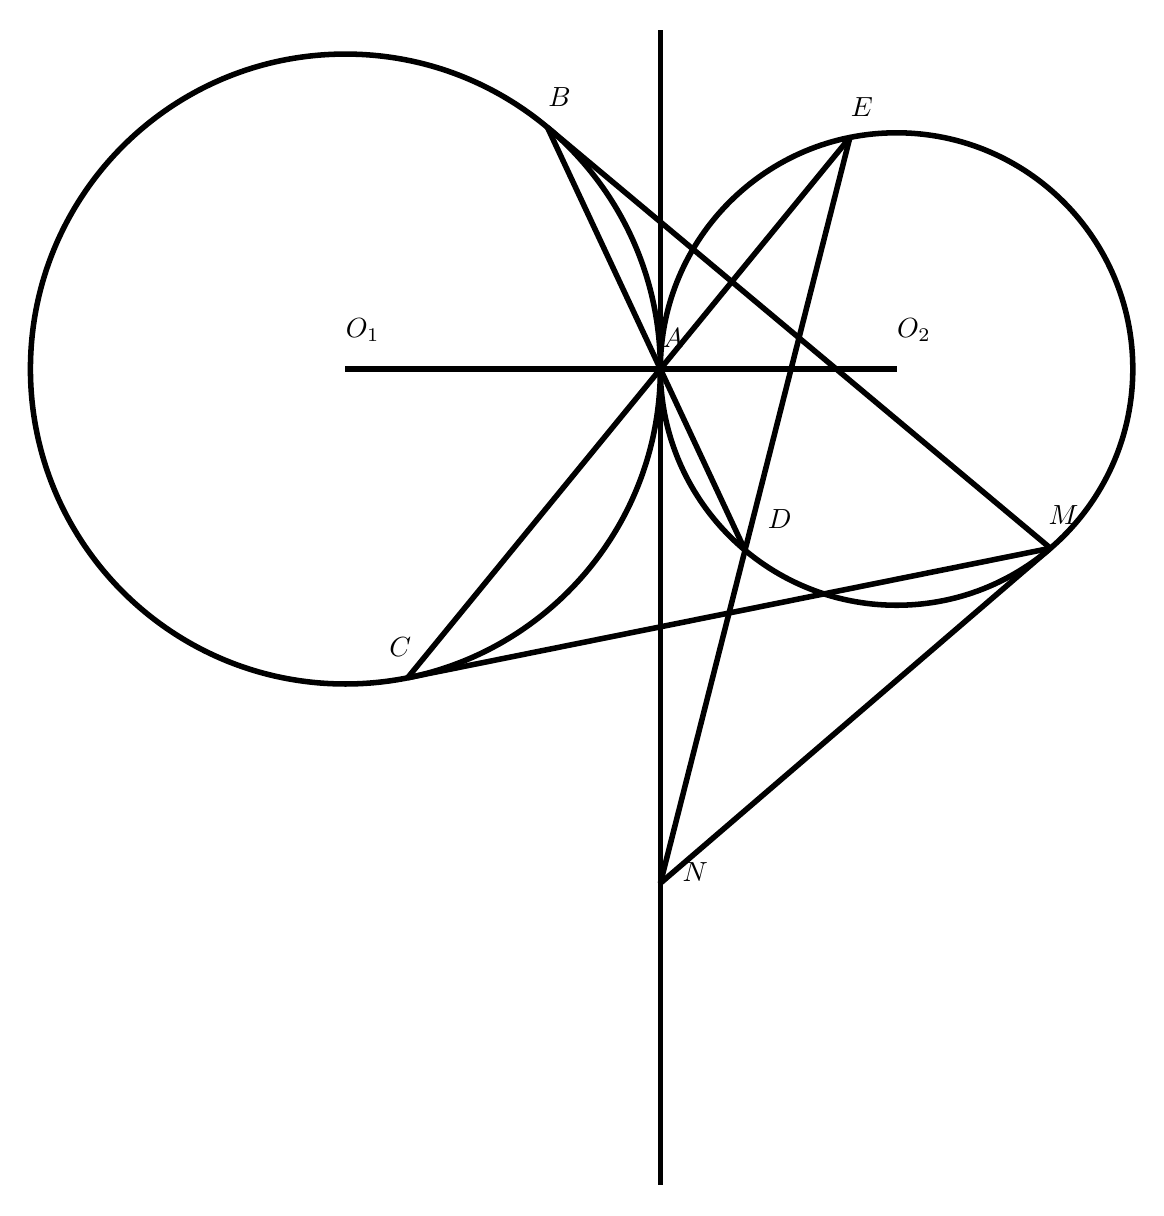
\begin{tikzpicture}
	\draw [line width=2pt] (-2,2) circle (4cm);
\draw [line width=2pt] (5,2) circle (3cm);
\draw [line width=2pt] (0.5666391124607006,5.067957572455484)-- (6.954410699743274,-0.27602258704280036);
\draw [line width=2pt] (6.954410699743274,-0.27602258704280036)-- (-1.2098529280724137,-1.9211819142605795);
\draw [line width=2pt] (-2,2)-- (5,2);
\draw [line width=2pt] (2,-8.36) -- (2,6.3);
\draw [line width=2pt] (0.5666391124607006,5.067957572455484)-- (3.0750206656544745,-0.300968179341613);
\draw [line width=2pt] (-1.2098529280724137,-1.9211819142605795)-- (4.40738969605431,4.940886435695435);
\draw [line width=2pt] (6.954410699743274,-0.27602258704280036)-- (2,-4.5303535139962685);
\draw [line width=2pt] (4.40738969605431,4.940886435695435)-- (2,-4.5303535139962685);
\draw (-1.78,2.49) node {$O_1$};
\draw (5.22,2.49) node {$O_2$};
\draw (2.16,2.39) node {$A$};
\draw (7.12,0.15) node {$M$};
\draw (0.72,5.45) node {$B$};
\draw (-1.04,-1.53) node [left] {$C$};
\draw (3.24,0.09) node [right] {$D$};
\draw (4.56,5.33) node {$E$};
\draw (2.16,-4.15) node [below right] {$N$};
	\end{tikzpicture}
\end{center}
\textbf{Lời giải.} Ta có hai tam giác \({O_1}AB\) và \({O_2}AD\) đồng dạng với nhau nên \(\widehat {A{O_1}B} = \widehat {A{O_2}D}.\)\\
Tương tự: \(\widehat {A{O_1}C} = \widehat {A{O_2}E}.\)\\
\( \Rightarrow \frac{{\overline {EC} }}{{\overline {DB} }} = \frac{{\overline {EA} }}{{\overline {DA} }}\).\\
Mà \(\widehat {MBA} = \frac{1}{2}\widehat {A{O_1}B} = \frac{1}{2}\widehat {A{O_2}D} = \widehat {AMD}.\) nên hai tam giác \(AMD\) và \(MBD\) đồng dạng.\\
\( \Rightarrow D{M^2} = \overline {DA} .\overline {DB} \). Tương tự: \(E{M^2} = \overline {EA} .\overline {EC} .\)\\
\( \Rightarrow \frac{{D{M^2}}}{{E{M^2}}} = \frac{{\overline {DA} .\overline {DB} }}{{\overline {EA} .\overline {EC} }} = \frac{{D{A^2}}}{{E{A^2}}} \Rightarrow \frac{{DM}}{{EM}} = \frac{{DA}}{{EA}}.\)\\
\( \Rightarrow \) Tứ giác \(AEMD\) là tứ giác điều hòa.\\
Mặt khác, \(N\) là giao điểm của \(DE\) và tiếp tuyến tại \(M\) của  \(\left( {{O_2}} \right)\) nên \(N\) thuộc tiếp tuyến chung tại \(A\) của hai đường tròn. Đường thẳng này cố định nên ta có đpcm.\\
\textbf{Nhận xét:} Đây là một bài toán khá hay và lời giải sử dụng tứ giác điều hòa khá đẹp mắt, ngoài cách giải bằng tứ giác điều hòa, ta có thể chứng minh bài toán bằng cách sử dụng phương tích, trục đẳng phương, chứng minh \(N\) là điểm đẳng phương của hai đường tròn \(\left( {{O_1}} \right),\left( {{O_2}} \right)\) và đường tròn điểm \(M\). Sau đây là một số bài toán về quỹ tích chứng minh bằng tính chất của tứ giác điều hòa.\\
\textbf{Ví dụ 9.1.} (Vietnam TST 2001) Trong mặt phẳng cho hai đường tròn \({\omega _1},{\omega _2}\) có tâm lần lượt là \({O_1},{O_2}\) cắt nhau tại hai điể \(A, B\). Các tiếp tuyến tại \(A, B\) của \({\omega _1}\) cắt nhau tại \(K\). Giả sử \(M\) là một điểm nằm trên \({\omega _1}\) nhưng không trùng với \(A, B\). Đường thẳng \(AM\) cắt \({\omega _2}\) tại điểm thứ hai \(P\), đường thẳng \(KM\) cắt \({\omega _1}\) tại điểm thứ hai \(C\) và đường thẳng \(AC\) cắt \({\omega _2}\) tại điểm thứ hai \(Q\).\\
a. Chứng minh rằng trung điểm của đoạn thẳng \(PQ\) nằm trên đường thẳng \(MC\).\\
b. Chứng minh rằng đường thẳng \(PQ\) luôn đi qua một điểm cố định khi \(M\) di chuyển trên \({\omega _1}\). \\
\textbf{Ví dụ 9.2} Từ một điểm \(M\) nằm ngoài \(\left( O \right)\) kẻ hai tiếp tuyến \(MB, MC\) đến đường tròn. \(A\) là một điểm cố định trên \(\left( O \right)\). Đường thẳng bất kì qua \(A\) cắt \(\left( O \right)\) tại \(G\), cắt \(MB, MC\) lần lượt tại \(D, E\), \(BE\) cắt \(CD\) tại \(S\). Chứng minh rằng \(GS\) luôn đi qua một điểm cố định. \\
\newline
\textbf{Ví dụ 10.} Đường tròn \(\left( I \right)\) nội tiếp tam giác \(ABC\) lần lượt tiếp xúc \(BC, CA, AB\) tại \(D, E, F\). \(AD\) cắt \(\left( I \right)\) tại điểm thứ hai \(P\). Cho rằng \(\widehat {BPC} = {90^ \circ }\), chứng minh rằng \(EA + AP = PD\). (China 2003)\\
\begin{center}
	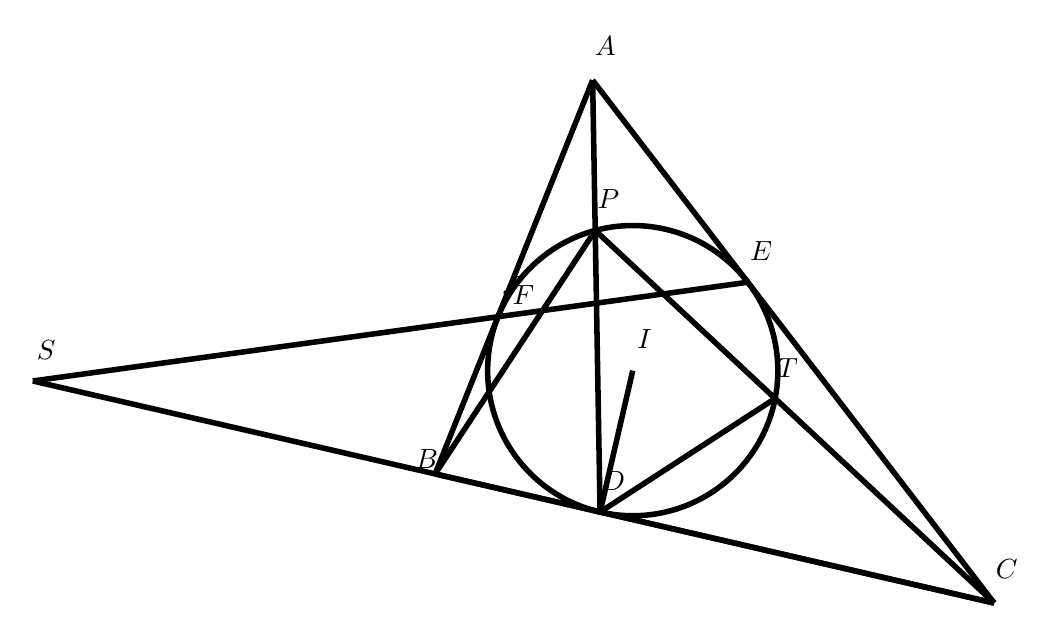
\begin{tikzpicture}
	\draw [line width=2pt] (-4,-2)-- (3.1,-3.64);
\draw [line width=2pt] (-1.4906433032076118,-0.6883578683445023) circle (1.842747543678488cm);
\draw [line width=2pt] (-2,3)-- (-4,-2);
\draw [line width=2pt] (3.1,-3.64)-- (-2,3);
\draw [line width=2pt] (-2,3)-- (-1.9053719782388632,-2.4838295712236995);
\draw [line width=2pt] (-4,-2)-- (-1.9670713272122484,1.091736187506519);
\draw [line width=2pt] (-1.9670713272122484,1.091736187506519)-- (3.1,-3.64);
\draw [line width=2pt] (0.31785665255035545,-1.041976900293478)-- (-1.9053719782388632,-2.4838295712236995);
\draw [line width=2pt] (-0.029219588454309886,0.4341211896738468)-- (-9.109298233328783,-0.8198240700479995);
\draw [line width=2pt] (-9.109298233328783,-0.8198240700479995)-- (3.1,-3.64);
\draw [line width=2pt] (-1.4906433032076118,-0.6883578683445023)-- (-1.9053719782388632,-2.4838295712236995);
\draw (3.26,-3.21) node {$C$};
\draw (-3.84,-1.57) node [below left] {$B$};
\draw (-1.84,3.43) node {$A$};
\draw (-1.34,-0.29) node {$I$};
\draw (-1.74,-2.09) node {$D$};
\draw (0.14,0.83) node {$E$};
\draw (-2.88,0.27) node {$F$};
\draw (-3.04,0.39) node {$J$};
\draw (-1.8,1.49) node {$P$};
\draw (-8.94,-0.43) node {$S$};
\draw (0.48,-0.65) node {$T$};
	\end{tikzpicture}
\end{center}
\textbf{Lời giải.} Gọi \(S\) là giao điểm của \(EF\) và \(BC\), \(T\) là giao điểm thứ hai của \(BC\) và \(\left( I \right)\).\\
Ta có: \(P\left( {BCDE} \right) =  - 1\), mà \(BP \bot PC\) \( \Rightarrow \) \(PC\) là tia phân giác của góc \(\widehat {DPS}\).\\
\( \Rightarrow \widehat {DPC} = \widehat {CPS} = \widehat {PDT}\).\\
\( \Rightarrow \) \(PT = DT\).\\
Lại có tứ giác \(PETD\) là tứ giác điều hòa nên \(PT.DE = 2PE.DT\) (định lí Ptolemy).\\
Mà \(PT = DT\) nên \(DE = 2PE\).\\
Mặt khác, hai tam giác \(AEP\) và \(ADE\) đồng dạng \\
\( \Rightarrow \) \(AD = 2AE\) và \(AE = 2AP\) suy ra: \(PD = EA + AP\).\\
\textbf{Nhận xét:} Đây là một bài toán hay, làm nổi bật tính chất của tứ giác điều hòa và định lí Ptolemy, vốn có quan hệ sâu sắc với nhau. Chìa khóa để giải bài toán này nằm ở việc tạo ra tứ giác \(PETD\) là tứ giác điều hòa và sử dụng các tính chất quen thuộc để suy ra các quan hệ độ dài. Mối liên kết giữa định lí Ptolemy và tứ giác điều hòa còn được thể hiện qua các bài toán sau:\\
\textbf{Ví dụ 10.1.} Cho tam giác \(ABC\) ngoại tiếp đường tròn \(\left( I \right)\), các tiếp điểm với \(BC, CA, AB\) lần lượt là \(D, E, F\). \(BE, CF\) lần lượt cắt \(\left( I \right)\) tại điểm thứ hai \(R, T\). Chứng minh rằng \(EF, BC, RT\) đồng quy.
\begin{center}
	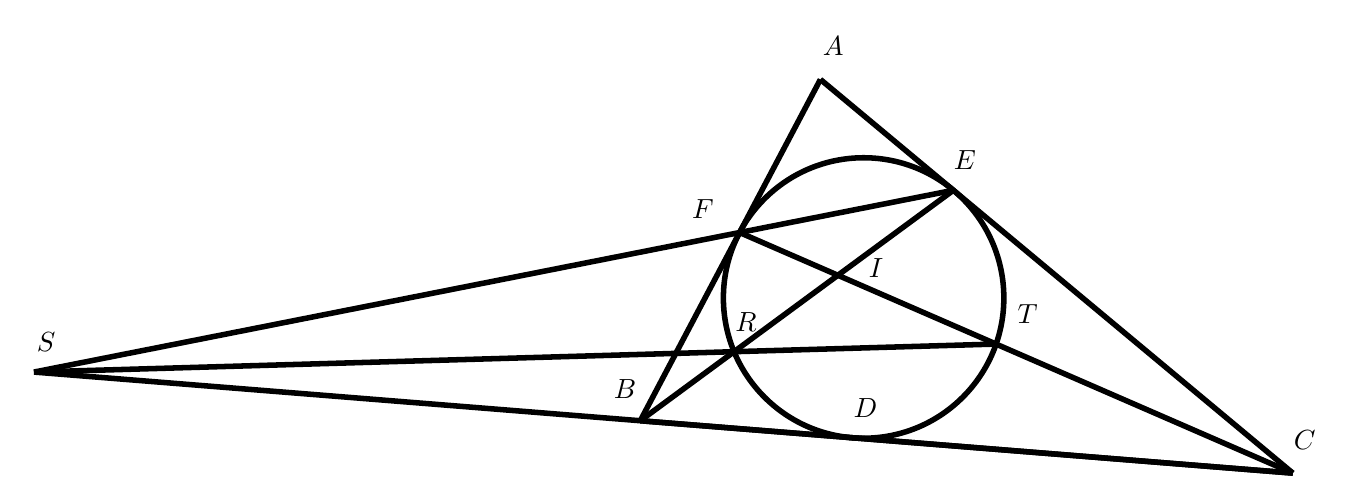
\begin{tikzpicture}
	\draw [line width=2pt] (-2,4)-- (-4.2875928276882105,-0.33463183115098816);
\draw [line width=2pt] (-4.2875928276882105,-0.33463183115098816)-- (4,-1);
\draw [line width=2pt] (4,-1)-- (-2,4);
\draw [line width=2pt] (-1.4511136391809414,1.2243201593565105) circle (1.7809478335468116cm);
\draw [line width=2pt] (-4.2875928276882105,-0.33463183115098816)-- (-0.31097861952801964,2.5924821829400164);
\draw [line width=2pt] (4,-1)-- (-3.0261761769612203,2.0555560993255613);
\draw [line width=2pt] (-0.31097861952801964,2.5924821829400164)-- (-11.987191417528528,0.2835293069636503);
\draw [line width=2pt] (-11.987191417528528,0.2835293069636503)-- (4,-1);
\draw [line width=2pt] (-11.987191417528528,0.2835293069636503)-- (0.2309355914181061,0.6390974909163396);
\draw (-1.8373539338812936,4.419998403260056) node {$A$};
\draw (-4.482056231958601,0.06401814760331198) node {$B$};
\draw (4.1521189176467255,-0.5777110864889762) node {$C$};
\draw (-1.292856401924201,1.6002790413393957) node {$I$};
\draw (-1.4289807849134744,-0.16933793752115642) node {$D$};
\draw (-0.1649686571559379,2.9809692116591675) node {$E$};
\draw (-3.4902928701796103,2.3586863179939184) node {$F$};
\draw (-2.945795338222518,0.9196571263930295) node {$R$};
\draw (0.3795288748011547,1.0168888285282247) node [right] {$T$};
\draw (-11.832772913379351,0.6668547008415221) node {$S$};
	\end{tikzpicture}
\end{center}
\textbf{Lời giải.} Gọi \(S, S'\) lần lượt là giao điểm của \(EF\) với \(BC, RT\).\\
Ta có: \(\frac{{\overline {SE} }}{{\overline {SF} }} = \frac{{D{E^2}}}{{D{F^2}}},\frac{{\overline {S'E} }}{{\overline {S'F} }} = \frac{{RE}}{{RF}}.\frac{{TE}}{{TF}}.\)\\
Theo định lí Ptolemy:\\
Tứ giác \(EFRD\) là tứ giác điều hòa \( \Rightarrow \frac{{RE}}{{RF}} = 2\frac{{DE}}{{DF}}.\)\\
Tứ giác \(EFDT\) là tứ giác điều hòa \( \Rightarrow \frac{{TE}}{{TF}} = \frac{{DE}}{{2DF}}.\)\\
\( \Rightarrow \frac{{\overline {SE} }}{{\overline {SF} }} = \frac{{\overline {S'E} }}{{\overline {S'F} }}\) \( \Rightarrow S \equiv S'.\)\\
Vậy ta có đpcm.\\
\textbf{Nhận xét:} Bản chất của bài toán trên chính là một bổ đề quen thuộc: Từ \(M\) ở ngoài đường tròn \(\left( O \right)\) kẻ hai cát tuyến \(MAB, MCD\), hai tiếp tuyến \(MP, MQ\) đến đường tròn. Chứng minh rằng \(PQ, AD, BC\) đồng quy.\\
\newline
\textbf{Ví dụ 10.2.} Cho tam giác \(ABC\) ngoại tiếp đường tròn \(\left( I \right)\), các tiếp điểm với \(BC, CA, AB\) lần lượt là \(D, E, F\). \(AD, CF\) lần lượt cắt đường tròn \(\left( I \right)\) tại điểm thứ hai \(H, K\). Chứng minh rằng \(\frac{{FD.HK}}{{FH.DK}} = 3.\)\\
\begin{center}
	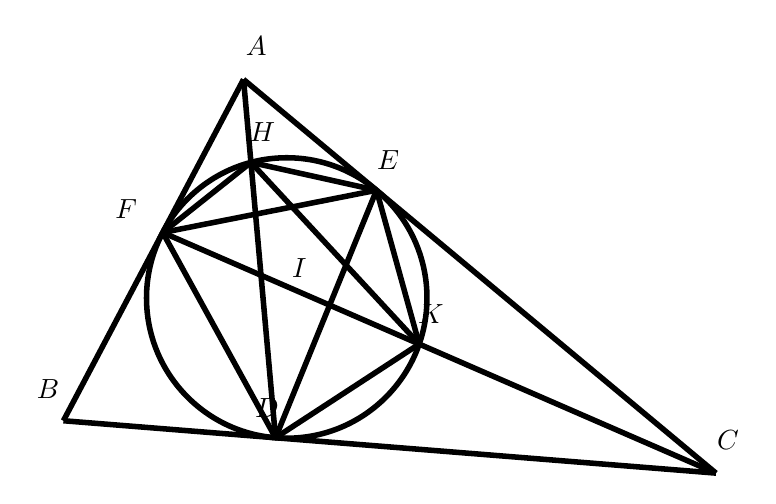
\begin{tikzpicture}
	\draw [line width=2pt] (-2,4)-- (-4.2875928276882105,-0.33463183115098816);
\draw [line width=2pt] (-4.2875928276882105,-0.33463183115098816)-- (4,-1);
\draw [line width=2pt] (4,-1)-- (-2,4);
\draw [line width=2pt] (-1.4511136391809414,1.2243201593565105) circle (1.7809478335468116cm);
\draw [line width=2pt] (4,-1)-- (-3.0261761769612203,2.0555560993255613);
\draw [line width=2pt] (-2,4)-- (-1.5936381791525718,-0.5509155831072775);
\draw [line width=2pt] (-3.0261761769612203,2.0555560993255613)-- (-1.5936381791525718,-0.5509155831072775);
\draw [line width=2pt] (-1.9059055481593514,2.9462201289664924)-- (0.2309355914181061,0.6390974909163396);
\draw [line width=2pt] (-1.9059055481593514,2.9462201289664924)-- (-3.0261761769612203,2.0555560993255613);
\draw [line width=2pt] (0.2309355914181061,0.6390974909163396)-- (-1.5936381791525718,-0.5509155831072775);
\draw [line width=2pt] (-1.9059055481593514,2.9462201289664924)-- (-0.31097861952801964,2.5924821829400164);
\draw [line width=2pt] (-0.31097861952801964,2.5924821829400164)-- (-1.5936381791525718,-0.5509155831072775);
\draw [line width=2pt] (-3.0261761769612203,2.0555560993255613)-- (-0.31097861952801964,2.5924821829400164);
\draw [line width=2pt] (-0.31097861952801964,2.5924821829400164)-- (0.2309355914181061,0.6390974909163396);
\draw (-1.8373539338812936,4.419998403260056) node {$A$};
\draw (-4.482056231958601,0.06401814760331198) node {$B$};
\draw (4.1521189176467255,-0.5777110864889762) node {$C$};
\draw (-1.292856401924201,1.6002790413393957) node {$I$};
\draw (-1.4289807849134744,-0.16933793752115642) node [left] {$D$};
\draw (-0.1649686571559379,2.9809692116591675) node {$E$};
\draw (-3.4902928701796103,2.3586863179939184) node {$F$};
\draw (-1.7595685721731376,3.33100333934587) node {$H$};
\draw (0.3795288748011547,1.0168888285282247) node {$K$};
	\end{tikzpicture}
\end{center}
\textbf{Lời giải.} Theo định lí Ptolemy:\\
Tứ giác \(FHED\) là tứ giác điều hòa \( \Rightarrow \) \(ED.FK = 2FE.DK\).\\
Tứ giác \(FEKD\) là tứ giác điều hòa \( \Rightarrow \) \(HD.FE = 2HF.DE\).\\
Nhân vế theo vế của hai đẳng thức trên, ta được: \(FK.HD = 4DK.HF\).\\
Mà \(FH.DK + FD.HK = FK.HD\).\\
Từ hai điều trên, ta có: \(FD.HK=3FH.DK\) (đpcm).\\
\textbf{Nhận xét:} Bài toán trên cho ta gợi ý về tính chất của các cặp tứ giác điều hòa có chung ba đỉnh, cụ thể trong lời giải trên là \(FHED\) và \(FEKD\). Mời bạn đọc đến với một kết quả đẹp sau đây phát triển từ ví dụ trên:\\
\textbf{Ví dụ 10.3.} Cho tam giác \(ABC\) ngoại tiếp đường tròn \(\left( I \right)\), các tiếp điểm với \(BC, CA, AB\) lần lượt là \(D, E, F\). \(AD\) cắt đường tròn \(\left( I \right)\) tại điểm thứ hai \(M\). Đường tròn ngoại tiếp tam giác \(MCD\) cắt \(DF\) tại điểm thứ hai \(N\). \(CN\) cắt \(AB\) tại \(G\). Chứng minh \(CD = 3FG\).\\
\begin{center}
	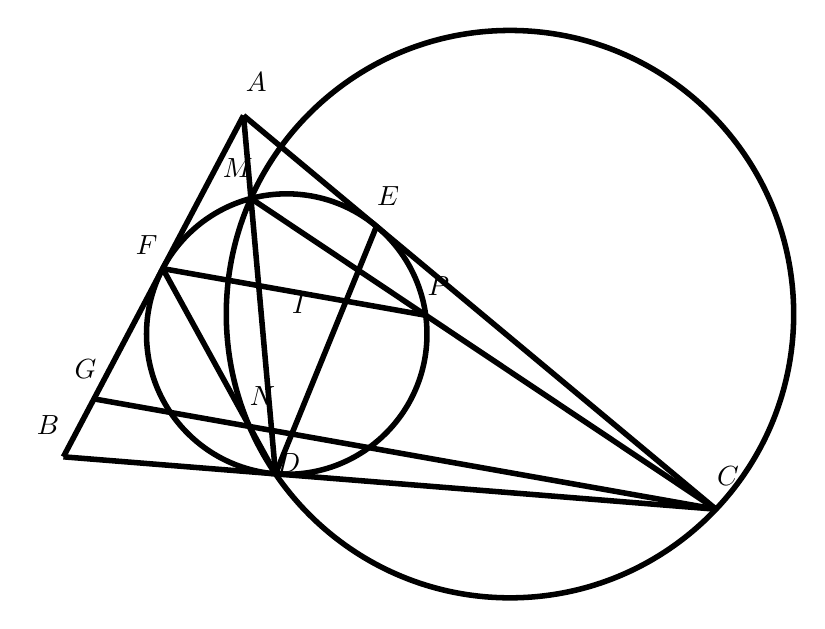
\begin{tikzpicture}
	\draw [line width=2pt] (-2,4)-- (-4.2875928276882105,-0.33463183115098816);
\draw [line width=2pt] (-4.2875928276882105,-0.33463183115098816)-- (4,-1);
\draw [line width=2pt] (4,-1)-- (-2,4);
\draw [line width=2pt] (-1.4511136391809414,1.2243201593565105) circle (1.7809478335468116cm);
\draw [line width=2pt] (-2,4)-- (-1.5936381791525718,-0.5509155831072775);
\draw [line width=2pt] (-3.0261761769612203,2.0555560993255613)-- (-1.5936381791525718,-0.5509155831072775);
\draw [line width=2pt] (-0.31097861952801964,2.5924821829400164)-- (-1.5936381791525718,-0.5509155831072775);
\draw [line width=2pt] (1.3840576236111353,1.4774791854300848) circle (3.602923483898366cm);
\draw [line width=2pt] (-3.8992307575398324,0.40125375604857655)-- (4,-1);
\draw [line width=2pt] (-1.9059055481593514,2.9462201289664924)-- (4,-1);
\draw [line width=2pt] (-3.0261761769612203,2.0555560993255613)-- (0.3137569579112099,1.4630814655488569);
\draw (-1.8373539338812936,4.419998403260056) node {$A$};
\draw (-4.482056231958601,0.06401814760331198) node {$B$};
\draw (4.1521189176467255,-0.5777110864889762) node {$C$};
\draw (-1.292856401924201,1.6002790413393957) node {$I$};
\draw (-1.4289807849134744,-0.16933793752115642) node [below] {$D$};
\draw (-0.1649686571559379,2.9809692116591675) node {$E$};
\draw (-3.4902928701796103,2.3586863179939184) node [right] {$F$};
\draw (-1.7595685721731376,3.33100333934587) node [left] {$M$};
\draw (-1.7595685721731376,0.43349861571705367) node {$N$};
\draw(-3.743095295731118,0.7835327434037563) node [left] {$G$};
\draw (0.4767605769363498,1.8336351264638642) node {$P$};
	\end{tikzpicture}
\end{center} 
\textbf{Lời giải.} Gọi \(P\) là giao điểm thứ hai của \(MC\) và đường tròn \(\left( I \right)\). Ta có \(FP\) song song với \(CG\).\\
\( \Rightarrow \frac{{FG}}{{CD}} = \frac{{FG}}{{CP}}.\frac{{CP}}{{CD}} = \frac{{\sin \widehat {PCG}}}{{\sin \widehat {FGC}}}.\frac{{\sin \widehat {PDC}}}{{\sin \widehat {DPC}}} = \frac{{\sin \widehat {DFP}}}{{\sin \widehat {FDP}}}.\frac{{\sin \widehat {FDM}}}{{\sin \widehat {DFM}}} = \frac{{PD}}{{PF}}.\frac{{MF}}{{MD}}.\)\\
Theo định lí Ptolemy:\\
Tứ giác \(FMED\) là tứ giác điều hòa \( \Rightarrow \) \(FM.ED = ME.FD\).\\
Tứ giác \(PEMD\) là tứ giác điều hòa \( \Rightarrow \) \(2EM.PD = MP.ED\).\\
Nhân vế theo vế hai đẳng thức trên, ta có: \(2FM.DP = FD.MP\).\\
Mà \(FM.DP + FD.MP = FP.MD\).\\
\( \Rightarrow \) \(3FM.DP = FP.DM\). \( \Rightarrow \) \(\frac{{FG}}{{CD}} = \frac{1}{3}.\) (đpcm)\\
\\
\textbf{Ví dụ 11.} Cho tam giác \(ABC\) ngoại tiếp đường tròn \(\left( I \right)\), các tiếp điểm với \(BC, CA, AB\) lần lượt là \(D, E, F\). \(AD\) cắt \(\left( I \right)\) tại điểm thứ hai \(X\). \(BX, CX\) theo thứ tự cắt \(\left( I \right)\) tại điểm thứ hai \(Y, Z\). \(AY, AZ\) lần lượt cắt \(\left( I \right)\) tại điểm thứ hai \(R, S\). Chứng minh rằng \(AD, ES, FR\) đồng quy.\\
\begin{center}
	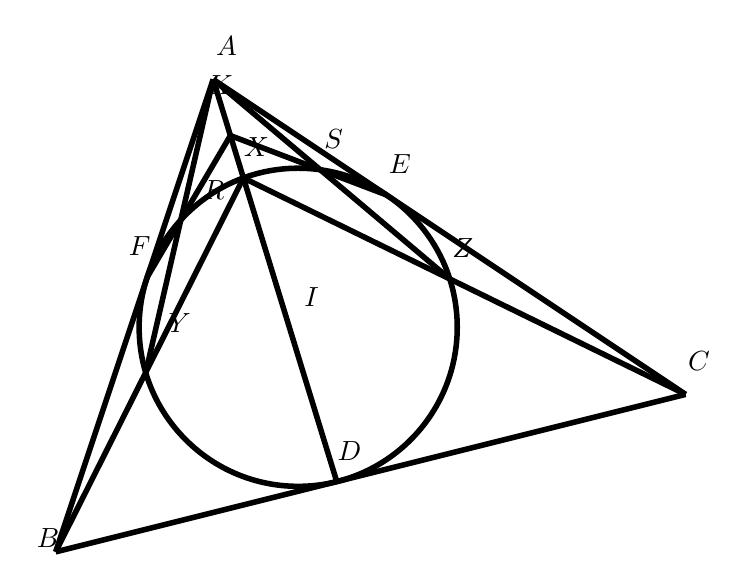
\begin{tikzpicture}
	\draw [line width=2pt] (-2,4)-- (-4,-2);
\draw [line width=2pt] (-4,-2)-- (4,0);
\draw [line width=2pt] (4,0)-- (-2,4);
\draw [line width=2pt] (-0.9199674881957767,0.8522060158698974) circle (2.0200286647829144cm);
\draw [line width=2pt] (-2,4)-- (-0.43003857339134344,-1.107509643347836);
\draw [line width=2pt] (-1.6153891355452572,2.7487567109324833)-- (-4,-2);
\draw [line width=2pt] (-1.6153891355452572,2.7487567109324833)-- (4,0);
\draw [line width=2pt] (-2,4)-- (-2.8564529478194256,0.2772800456695339);
\draw [line width=2pt] (-2,4)-- (1.004443683287734,1.466337475424043);
\draw [line width=2pt] (-1.7808508713672968,3.287048542179363)-- (-2.8363349440586085,1.4909951678241748);
\draw [line width=2pt] (-1.7808508713672968,3.287048542179363)-- (0.20054280853989423,2.5329714609734038);
\draw (-1.83,4.42) node {$A$};
\draw (-3.83,-1.58) node [below left] {$B$};
\draw (4.17,0.42) node {$C$};
\draw(-0.75,1.24) node {$I$};
\draw (-0.27,-0.72) node {$D$};
\draw (0.37,2.92) node {$E$};
\draw (-2.67,1.88) node [left] {$F$};
\draw (-1.45,3.14) node {$X$};
\draw (-2.69,0.66) node [above right] {$Y$};
\draw (1.17,1.86) node {$Z$};
\draw (-2.25,2.6) node [right] {$R$};
\draw (-0.47,3.24) node {$S$};
\draw(-1.63,3.68) node [above left] {$K$};
	\end{tikzpicture}
\end{center}
\textbf{Lời giải.} Gọi \(K\) là giao điểm của \(ES\) và \(AD\).\\
Tứ giác \(ZEXD\) là tứ giác điều hòa và \(S\) là một điểm thuộc đường tròn ngoại tiếp tứ giác \(ZEXD\) nên \(S\left( {ZEXD} \right) =  - 1.\)\\
\( \Rightarrow \left( {AXKD} \right) = S\left( {AXKD} \right) = S\left( {ZEXD} \right) =  - 1.\)\\
Gọi \(K'\) là giao điểm của \(FR\) và \(AD\). Tương tự như trên, ta được \(\left( {AXK'D} \right)  = -1\).\\
\( \Rightarrow K \equiv K'.\) Vậy \(AD, ES, FR\) đồng quy.\\
\newline
\textbf{Ví dụ 12.} (IMO 2002) Cho tam giác \(ABC\) ngoại tiếp đường tròn \(\left( I \right)\), các tiếp điểm với \(BC, CA, AB\) lần lượt là \(D, E, F\). Gọi \(G\) là trung điểm của đường cao \(AH\). \(DG\) cắt \(\left( I \right)\) tại điểm thứ hai \(T\). Chứng minh rằng đường tròn ngoại tiếp tam giác \(TBC\) tiếp xúc với đường tròn \(\left( I \right)\).\\
\begin{center}
	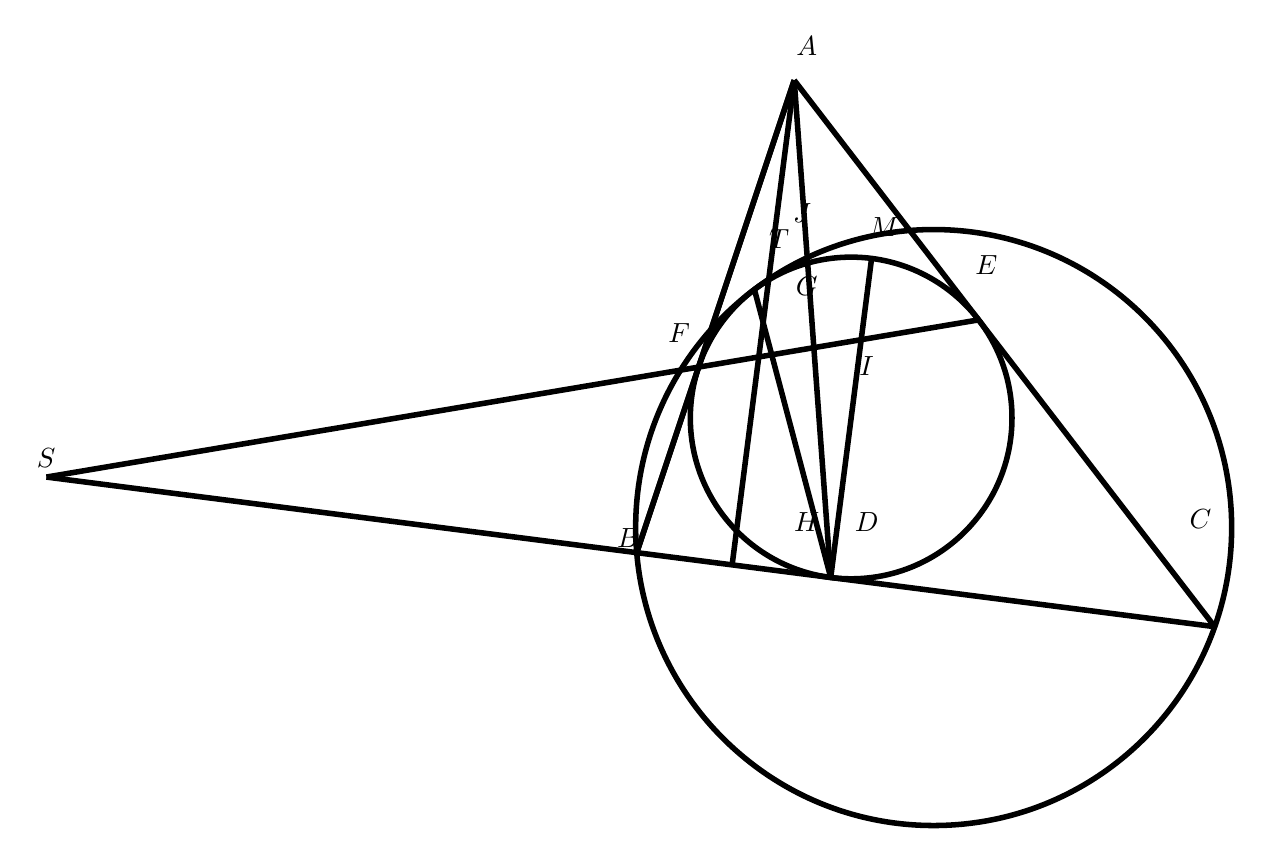
\begin{tikzpicture}
	\draw [line width=2pt] (-2,3)-- (-4,-3);
\draw [line width=2pt] (-2,3)-- (-4,-3);
\draw [line width=2pt] (-4,-3)-- (3.34,-3.94);
\draw [line width=2pt] (3.34,-3.94)-- (-2,3);
\draw [line width=2pt] (-1.2767371404527357,-1.2894752232791138) circle (2.0425985621948755cm);
\draw [line width=2pt] (-2,3)-- (-2.7882657160805855,-3.1551812298207427);
\draw [line width=2pt] (-0.22895941987962345,-2.681023555230252) circle (3.7845069730722622cm);
\draw [line width=2pt] (-2.505383406914281,0.342283716696604)-- (-1.5362042585289566,-3.3155269750657737);
\draw [line width=2pt] (-11.496350612465433,-2.0399768970412118)-- (0.3421020108736435,-0.04385542237136443);
\draw [line width=2pt] (-4,-3)-- (-11.496350612465433,-2.0399768970412118);
\draw [line width=2pt] (-2,3)-- (-1.5362042585289566,-3.3155269750657737);
\draw [line width=2pt] (-1.017270022376515,0.736576528507546)-- (-1.5362042585289566,-3.3155269750657737);
\draw (-1.84,3.43) node {$A$};
\draw (-3.84,-2.57) node [below left] {$B$};
\draw (3.16,-2.57) node {$C$};
\draw (-1.08,-0.63) node {$I$};
\draw (-1.08,-2.61) node {$D$};
\draw (0.44,0.65) node {$E$};
\draw (-3.46,-0.45) node [above] {$F$};
\draw(-1.84,-2.61) node {$H$};
\draw (-1.84,0.39) node {$G$};
\draw (-2.19,0.74) node [above] {$T$};
\draw (-0.86,1.13) node {$M$};
\draw (-1.66,1.07) node [above left] {$J$};
\draw (-11.5,-2.04) node [above] {$S$};
	\end{tikzpicture}
\end{center}
\textbf{Lời giải.} Gọi \(S\) là giao điểm của \(BC\) và \(EF\), \(J\) là giao điểm thứ hai của \(AD\) với đường tròn \(\left( I \right)\), \(M\) là giao điểm của đoạn thẳng \(AI\) và đường tròn \(\left( I \right)\). \\
Ta có: \(D\left( {MGAH} \right) =  - 1\) (chùm điều hòa trung tuyến) nên tứ giác \(MTJD\) là tứ giác điều hòa.\\
\(SJ\) là tiếp tuyến của đường tròn \(\left( I \right)\) do tứ giác \(JFDE\) là tứ giác điều hòa.\\
Nên \(SD\) là tiếp tuyến của \(\left( I \right)\).\\
\( \Rightarrow \) \(S, T, M\) thẳng hàng, mà \(SM \bot TD\) nên \(TD\) là phân giác trong của góc \(\widehat {BTC}.\)\\
Gọi \(L\) là tâm đường tròn ngoại tiếp tam giác \(TBC\), \(Q\) là điểm chính giữa cung \(BC\) không chứa \(T\) của đường tròn này thì \(T, D, Q\) thẳng hàng và \(LQ\) song song với \(ID\).\\
Suy ra: \(\widehat {DTI} = \widehat {TDI} = \widehat {TQL} = \widehat {QTL}.\)\\
Do đó, \(T, I, L\) thẳng hàng. Từ đó, ta có đpcm.\\
\textbf{Nhận xét:} Đây là một bài toán hay và điển hình cho ứng dụng của tứ giác điều hòa xuất hiện trong kì thi Olympic Toán quốc tế, sau đây xin đưa ra một kết quả khác được phát triển dựa trên bài toán trên.\\
\textbf{Ví dụ 12.1} (Đề chọn đội tuyển Hải Phòng 2016 - 2017)\\
 Cho tam giác nhọn \(ABC\), \(\left( AB < AC \right)\), phân giác trong đỉnh \(A\) cắt \(BC\) tại \(D\), \(E\) là điểm trên đoạn \(BC\) sao cho \(BD = BE\). Phân giác ngoài tại đỉnh \(A\) cắt đường thẳng qua \(D\) và vuông góc với \(BC\) tại \(F\). \(I\) là trung điểm của \(DF\), đường thẳng \(EI\) cắt \(AD\) tại \(M\), đường thẳng \(EF\) cắt đường thẳng qua \(M\) và vuông góc với \(BC\) tại \(K\).\\
a. Đường thẳng \(AF\) cắt đường thẳng \(BC\) tại \(P\), \(KD\) cắt đường tròn đường kính \(DF\) tại điểm thứ hai \(L\). Chứng minh rằng đường thẳng \(PL\) tiếp xúc với đường tròn đường kính \(DF\).\\
b. Chứng minh rằng \(I\) là tâm đường tròn nội tiếp tam giác \(KBC\).
\newpage
\section{Bài tập rèn luyện.}
\textbf{Bài 1.} Cho tam giác \(ABC\) có trực tâm \(H\). Gọi \(D\) là giao điểm của \(BH\) và \(AC\), \(E\) là giao điểm của \(CH\) và \(AB\). Đường tròn ngoại tiếp tam giác \(ADE\) cắt đường tròn ngoại tiếp tam giác \(ABC\) tại điểm \(F\) khác \(A\). Chứng minh rằng phân giác trong các góc \(\widehat {BFC},\widehat {BHC}\) cắt nhau tại một điểm trên \(BC\).\\
\textbf{Bài 2.} (IMO 2003) Cho tứ giác \(ABCD\) nội tiếp. Gọi \(P, Q, R\) là lần lượt là chân đường vuông góc kẻ từ \(D\) đến \(BC, CA, AB\). Chứng minh rằng \(PQ = QR\) khi và chỉ khi phân giác các góc \(\widehat {ABC},\widehat {ADC}\) cắt nhau tại một điểm trên \(AC\).\\
\textbf{Bài 3.} Cho tam giác \(ABC\) ngoại tiếp \(\left( I \right)\), \(\left( I \right)\) tiếp xúc với \(BC, CA, AB\) lần lượt tại \(D, E, F\). \(AD\) cắt \(\left( I \right)\) tại điểm thứ hai \(M\).\(BM, CM\) cắt \(\left( I \right)\) lần lượt tại \(Y, Z\). Chứng minh rằng \(BZ, CY, AD\) đồng quy. \\
\textbf{Bài 4.} (Vietnam TST 2002) Trong mặt phẳng cho hai đường tròn \({\omega _1}\) tâm \(O\) và \({\omega _2}\) tâm \(O'\) cắt nhau tại \(A\) và \(B\). Các tiếp tuyến tại \(A, B\) của \({\omega _1}\) cắt nhau tại \(K\). Giả sử \(M\) là một điểm nằm trên \({\omega _1}\) nhưng không trùng với \(A\) và \(B\). Đường thẳng \(AM\) cắt \({\omega _2}\) tại điểm thứ hai \(P\), đường thẳng \(KM\) cắt \({\omega _1}\) tại điểm thứ hai \(C\) và đường thẳng \(AC\) cắt \({\omega _2}\) tại điểm thứ hai \(Q\).\\
a. Chứng minh rằng trung điểm \(PQ\) thuộc đường thẳng \(MC\).\\
b. Chứng minh rằng đường thẳng \(PQ\) luôn đi qua một điểm cố định khi \(M\) thay đổi trên \({\omega _1}\).\\
\textbf{Bài 5.} (China TST 2008) Cho tam giác \(ABC\) nhọn có đường tròn \(\left( I \right)\) nội tiếp. \(M, N\) là trung điểm của cung nhỏ \(AC, AB\) của đường tròn \(\left( O \right)\) ngoại tiếp tam giác \(ABC\), \(D\) là trung điểm của \(MN\). Gọi \(G\) là điểm tùy ý trên cung nhỏ \(BC\) của \(\left( O \right)\). Gọi \({I_1}, {I_2}\) lần lượt là tâm đường tròn nội tiếp của các tam giác \(ABG, ACG\). \(P\) là giao điểm thứ hai của \(\left( O \right)\) và đường tròn ngoại tiếp tam giác \(G{I_1}{I_2}\). Chứng minh rằng \(P, I, D\) thẳng hàng.\\
\textbf{Bài 6.} Cho tam giác \(ABC\) nội tiếp đường tròn \(\left( O \right)\), ngoại tiếp đường tròn \(\left( I \right)\), \(AD\) là đường phân giác trong. \(\left( K \right)\), \(\left( L \right)\) lần lượt là đường tròn nội tiếp tam giác \(ABD, ACD\), \(J\) là tâm đường tròn ngoại tiếp tam giác \(AKL\). \(IJ\) cắt đường tròn ngoại tiếp tam giác \(IKL\) tại \(P\) khác \(I\). Chứng minh rằng tâm đường tròn ngoại tiếp tam giác \(PBC\) nằm trên  \(\left( O \right)\).
\newpage
\section{Tài liệu tham khảo.}
1. Tài liệu chuyên Toán Hình học 10 - Đoàn Quỳnh (chủ biên) - NXB Giáo dục Việt Nam 2011.\\
2. Chuyên đề Tứ giác điều hòa - lớp 10 Toán Khóa 17 - THPT Chuyên Lê Quý Đôn - Bình Định.\\
3. Chuyên đề Tứ giác điều hòa - Nguyễn Việt Hà (THPT Chuyên Lào Cai).\\
4. Chuyên đề Tứ giác điều hòa - Phan Nguyễn Văn Trường, Lục Đình Khánh, Bùi Hà Đăng Quang - Trường Phổ thông Năng khiếu - ĐHQG TPHCM.\\
5. Julielltv Blog (Blog của chuyên Hà Tĩnh) - https://julielltv.wordpress.com\\
6. Chuyên đề Tứ giác điều hòa - diễn đàn Mathcopes (chuyên KHTN).\\
7. dinhtrungphan.blogspot.com/2014/06/bai-toan-1-e-thi-olympic-duyen-hai-bac.html
\newpage
\section{Lời kết}
\textit{Các bạn thân mến, qua những bài tập trên, chúng ta thấy được vẻ đẹp của tứ giác điều hòa trong hình học. Tứ giác điều hòa là một công cụ mạnh giúp chúng ta có thể dễ dàng giải quyết các bài khó, nếu nắm vững kiến thức về tứ giác điều hòa, chúng ta có thể tạo ra nhiều bài toán "hay" và "đẹp".\\
Để hoàn thành chuyên đề này, chúng em nhận được nhiều sự giúp đỡ, quan tâm của mọi người, đặc biệt là thầy Trần Quang Vinh - người đã tận tình hướng dẫn để chúng em có thể hoàn tất chuyên đề. Đây là lần đầu nhóm chúng em làm chuyên đề Toán với nội dung về Tứ giác điều hoa - một chuyên đề hay và quan trọng. Có thể kiến thức cung cấp ở trên chưa thực sự đầy đủ, đôi chỗ bài tập giải chưa đầy đủ, chi tiết như mong muốn nhưng đó đã là nỗ lực trong quá trình tìm hiểu của cả nhóm. Dù vậy, chuyên đề chắc chắn không tránh khỏi những thiếu sót, chúng em rất mong nhận được đóng góp quý báu của các thầy cô và các bạn để kiến thức trong lĩnh vực này của chúng em được hoàn thiện hơn. Hi vọng chuyên đề này sẽ mang lại được nhiều điều bổ ích cho bạn đọc.\\
Xin chân thành cảm ơn!}\\
\begin{flushright}
\textbf{Nhóm tác giả}
\end{flushright}
\end{document}
\documentclass[12pt,a4paper]{article}
\usepackage[utf8]{vietnam}
\usepackage{amsmath}
\usepackage{amsfonts}
\usepackage{amssymb}
\usepackage{tikz, tkz-euclide, tkz-tab}
\usepackage{pgf,pgfplots}
\pgfplotsset{compat=1.15}
\usetikzlibrary{calc,intersections,patterns,arrows,shapes}
\usepackage{graphicx}
\usepackage[unicode]{hyperref}
\usepackage[left=2cm,right=2cm,top=2cm,bottom=2cm]{geometry}
\begin{document}
\begin{center}
\textbf{TRƯỜNG THPT CHUYÊN LÊ QUÝ ĐÔN - BÀ RỊA - VŨNG TÀU}\\
\textbf{LỚP 10 TOÁN 1 (2017-2018)}\\
\end{center}
\begin{center}
\fontsize{20}{18}\selectfont
Chuyên đề\\
\textbf{TỨ GIÁC ĐIỀU HÒA VÀ ỨNG DỤNG GIẢI TOÁN HÌNH HỌC}
\end{center}
\begin{center}
\begin{tikzpicture}
	\draw [ultra thick] (-3,3)node [above left] {$A$}--(5,5)node [above 		right] {$B$};
	\draw [ultra thick] (5,5)--(8,-2)node [below right] {$C$};
	\draw [ultra thick] (8,-2)--(-5,-2)node [below left] {$D$};
	\draw [ultra thick] (-5,-2)--(-3,3);
\end{tikzpicture}
\end{center}
\begin{flushright}
Vũng Tàu, tháng 11 - 12 năm 2017
\end{flushright}
\textbf{Giáo viên hướng dẫn:} Thầy Trần Quang Vinh, Giáo viên trường THPT Chuyên Lê Quý Đôn.\\
\textbf{Học sinh thực hiện:}
Lê Khánh Duy\\
Nguyễn Mai Gia Hân\\
Nguyễn Văn Lộc\\
\newpage
\tableofcontents
\newpage
\section{Lời mở đầu}
\textit{Tứ giác điều hòa là một tứ giác nội tiếp đặc biệt, thú vị trong hình học, do đó nó là một chủ đề không thể thiếu trong hình học Euclide cổ điển (nếu coi đường thẳng là đường tròn suy rộng thì tứ giác điều hòa là một khái niệm xuất phát từ hàng điểm điều hòa, tỉ số kép. Tứ giác điều hòa có ứng dụng khá lớn trong các bài toán định tính như chứng minh thẳng hàng, đồng quy, song song, vuông góc, trung điểm, chứng minh đi qua điểm cố định và các bài toán về chứng minh hệ thức trong hình học... Đây là một công cụ xuất sắc mà bất kì người yêu Toán nào cũng nên biết và nắm vững, được sử dụng để mang đến nhiều lời giải "đẹp". Rất nhiều các bài toán hình học trong các cuộc thi Olympic Toán gần đây chứa đựng trong nó các ý tưởng về tứ giác điều hòa. Chính vì vậy nhóm chúng em đã nghiên cứu và viết thành chuyên đề này với hi vọng đem lại cho bạn đọc đầy đủ những ứng dụng của tứ giác điều hòa.}
\begin{flushright}
\textbf{Nhóm tác giả}
\end{flushright}
\newpage
\section{Kiến thức chuẩn bị.}
\subsection{Các kiến thức cơ bản về véc-tơ, độ dài đại số, các định lí cơ bản.}
\subsection{Hàng điểm điều hòa và chùm điều hòa.}
\subsubsection{Hàng điểm điều hòa.}
Cho bốn điểm \(A, B, C, D\) phân biệt trên trục. Ta định nghĩa tỉ số kép \(\left( {ABCD} \right)\) là \(\frac{{\overline {AC} }}{{\overline {AD} }}:\frac{{\overline {BC} }}{{\overline {BD} }}.\)\\
Nếu \(\left( {ABCD} \right) =  - 1\) thì ta nói \(A, B, C, D\) lập thành hàng điểm điều hòa.\\
\textbf{\textit{*Hai dạng hàng điểm điều hòa cơ bản.}}\\
i. Cho tam giác \(ABC\) không cân có phân giác \(AD, AE\) \(\left( {D,E \in BC} \right)\) thì ta có: \(\left( {EDBC} \right) =  - 1.\)
\begin{center}
	\begin{tikzpicture}
	\draw(-4,4)node [above] {$A$}--(-2,0)node [below] {$B$};
	\draw(-2,0)--(6,0)node [below] {$C$}--(-4,4);
	\draw(-4,4)--(0.35,0)node [below] {$D$};
	\draw(-4,4)--(-7.68,0)node [below] {$E$}--(-2,0);
	\end{tikzpicture}
\end{center}
ii. Tứ giác \(ABCD\) có \(AB\) cắt \(CD\) tại \(F\), \(AD\) cắt \(BC\) tại \(E\), \(AC\) cắt \(BD\) tại \(I\), \(EI\) cắt \(CD\) tại \(K\). Khi đó: \(\left( {FKDC} \right) =  - 1.\) 
\begin{center}
	\begin{tikzpicture}
	\draw(-3,2)node [above left] {$A$}--(3,5)node [above right] {$B$}--(6,0)node [below right] {$C$}--(-5,0)node [below left] {$D$}--(-3,2);
	\draw(6,0)--(1.88,6.88)node [above] {$E$}--(-5,0);
	\draw(3,5)--(-7,0)node [above left] {$F$}--(6,0);
	\draw(1.88,6.88)--(-3.53,0)node [below]  {$K$}--(-2.11,1.8)node  [below] {$I$};
	\draw(-3,2)--(6,0);
	\draw(3,5)--(-5,0);
	\end{tikzpicture}
\end{center}
\textbf{\textit{*Một vài dấu hiệu nhận biết hàng điểm điều hòa.}}\\
Cho \(A\left( a \right);B\left( b \right);C\left( c \right);D\left( d \right)\) trên trục. Khi đó \(\left( {ABCD} \right) =  - 1\) khi và chỉ khi một trong các điều kiện sau được thỏa mãn:
i. \(\left( {a + b} \right)\left( {c + d} \right) = 2\left( {ab + cd} \right)\) (Lagrange).\\
ii. \(\frac{1}{{\overline {AC} }} + \frac{1}{{\overline {AD} }} = \frac{2}{{\overline {AB} }}\) (Descartes).\\
iii. \(\overline {MC} .\overline {MD}  = M{A^2}\) với \(M\) là trung điểm \(AB\) (Newton).\\\
iv. \(\overline {AC} .\overline {AD}  = \overline {AB} .\overline {AI} \) với \(I\) là trung điểm \(CD\) (Maclaurin).\\
\textbf{\textit{*Phép chiếu xuyên tâm bảo toàn hàng điểm điều hòa.}}\\
Cho \(\left( {ABCD} \right) =  - 1\) và điểm \(S \notin \left( {ABCD} \right).\) Đường thẳng \(d\) bất kì không qua \(S\) cắt \(SA, SB, SC, SD\) lần lượt tại \(A_1, B_1, C_1, D_1\). Khi đó \(\left( {{A_1}{B_1}{C_1}{D_1}} \right) =  - 1.\)
\subsubsection{Chùm điều hòa.}
Cho \(\left( {ABCD} \right) =  - 1\) và điểm \(S \notin \left( {ABCD} \right).\) Bốn đường \(SA, SB, SC, SD\) lập thành chùm điều hòa đỉnh \(S\). \\
Kí hiệu: \(\left( {SA,SB,SC,SD} \right) =  - 1\) hoặc \(S\left( {ABCD} \right) =  - 1.\)
\textbf{\textit{*Hai dạng chùm điều hòa cơ bản.}}\\
\textit{i. Chùm trung tuyến.} Cho tam giác \(ABC\) có \(M\) là trung điểm \(BC\), \(Ad\) song song với \(BC\). Khi đó: \(\left( {AB,AC,AM,Ad} \right) =  - 1.\)
\begin{center}
	\begin{tikzpicture}
	\draw(-1,4)node [above left] {$A$}--(-3,-1)node [below left] 
	{$B$}--(4,-1)node [below right] {$C$}--(-1,4);
	\draw(-1,4)--(0.5,-1)node [below] {$M$};
	\draw(-1,4)--(4,4)node [above right] {$d$};
	\end{tikzpicture}
\end{center}
\textit{ii. Chùm phân giác.} Cho \(Sb, Sd\) là hai tia phân giác của góc \(\widehat {aSc}\). Khi đó: \(S\left( {abcd} \right) =  - 1.\)
\begin{center}
	\begin{tikzpicture}
	\draw(-1,4)node [above left] {$S$}--(-3,-1)node [left] 
	{$a$};
	\draw(-1,4)--(4,-1)node [right] {$c$};
	\draw(-1,4)--(0.03,-1)node [above left] {$b$};
	\draw(-1,4)--(4,5.03)node [above right] {$d$};
	\end{tikzpicture}
\end{center}
\subsection{Tỉ số kép với góc định hướng.}
\textit{Định lí 1 (Định lí Ceva dạng lượng giác).} Cho tam giác \(ABC\) và các điểm \(M, N, P\) theo thứ tự thuộc các đường thẳng \(BC, CA, AB\) (nhưng không trùng với đỉnh của tam giác). Khi đó, \(AM, BN, CP\) đồng quy hoặc đôi một song song nếu và chỉ nếu \(\frac{{\sin \left( {\overrightarrow {AM} ;\overrightarrow {AB} } \right)}}{{\sin \left( {\overrightarrow {AM} ;\overrightarrow {AC} } \right)}}.\frac{{\sin \left( {\overrightarrow {BN} ;\overrightarrow {BC} } \right)}}{{\sin \left( {\overrightarrow {BN} ;\overrightarrow {BA} } \right)}}.\frac{{\sin \left( {\overrightarrow {CP} ;\overrightarrow {CA} } \right)}}{{\sin \left( {\overrightarrow {CP} ;\overrightarrow {CB} } \right)}} = 1.\)\\
\textit{Hệ quả:} Khi \(M, N, P\) theo thứ tự thuộc các đường thẳng \(BC, CA, AB\) và không trùng với hai đầu mút của các đoạn thẳng này thì \(AM, BN, CP\) đồng quy khi và chỉ khi \(\frac{{\sin \widehat {MAB}}}{{\sin \widehat {MAC}}}.\frac{{\sin \widehat {NBC}}}{{\sin \widehat {NBA}}}.\frac{{\sin \widehat {PCA}}}{{\sin \widehat {PCB}}} = 1.\)\\
\textit{Định lí 2.} Với mọi chùm \(O\left( {ABCD} \right)\), ta có \(O\left( {ABCD} \right) = \frac{{\sin \left( {\overrightarrow {OC} ;\overrightarrow {OA} } \right)}}{{\sin \left( {\overrightarrow {OC} ;\overrightarrow {OB} } \right)}}:\frac{{\sin \left( {\overrightarrow {OD} ;\overrightarrow {OA} } \right)}}{{\sin \left( {\overrightarrow {OD} ;\overrightarrow {OB} } \right)}}.\)\\
\textit{Tỉ số kép với góc định hướng.} Cho bốn điểm phân biệt \(A, B, C, D\) cố định trên đường tròn \(\left( O \right)\) và điểm \(M\) thay đổi trên \(\left( O \right)\) thì \(M\left( {ABCD} \right)\) không đổi (khi \(M\) trùng với \(A, B, C, D\) thì \(MA, MB, MC, MD\) tương ứng được coi là tiếp tuyến của \(\left( O \right)\) tại \(A, B, C, D\)). 
\newpage
\section{Tứ giác điều hòa.}
\subsection{Định nghĩa.} Tứ giác nội tiếp \(ABCD\) được gọi là tứ giác điều hòa nếu tồn tại điểm \(M\) thuộc đường tròn ngoại tiếp tứ giác sao cho \(M\left( {ABCD} \right) =  - 1\), cũng tức là \(\left( {ABCD} \right) =  - 1\).\\
Như vậy, nếu tứ giác \(ABCD\) là tứ giác điều hòa thì \(M\left( {ABCD} \right) =  - 1\) với mọi điểm \(M\) thuộc đường tròn ngoại tiếp tứ giác.
\subsection{Tính chất.} 
Cho tứ giác \(ABCD\) nội tiếp đường tròn \(\left( O \right)\). Gọi \({\Delta _a},{\Delta _b},{\Delta _c},{\Delta _d}\) lần lượt là tiếp tuyến với \(\left( O \right)\) tại \(A, B, C, D\). Khi đó, các điều kiện sau đây là tương đương:\\
a. Tứ giác \(ABCD\) là tứ giác điều hòa.\\
b. \(AB.CD = AD. BC\).\\
c. \({\Delta _a}, {\Delta_c}, BD\) đồng quy và \({\Delta_b}, {\Delta_d}, AC\) đồng quy.\\
d. Các phân giác của các góc \(\widehat {BAD},\widehat {BCD}\) cắt nhau tại một điểm trên đường chéo \(BD\), các phân giác của các góc \(\widehat {ABC},\widehat {ADC}\) cắt nhau tại một điểm trên đường chéo \(AC\).\\
e. \(\widehat {MAD} = \widehat {BCA}\) với \(M\) là trung điểm \(BD\). Tương tự với trung điểm \(AC\).
\subsection{Chứng minh tính chất.}
\begin{center}
	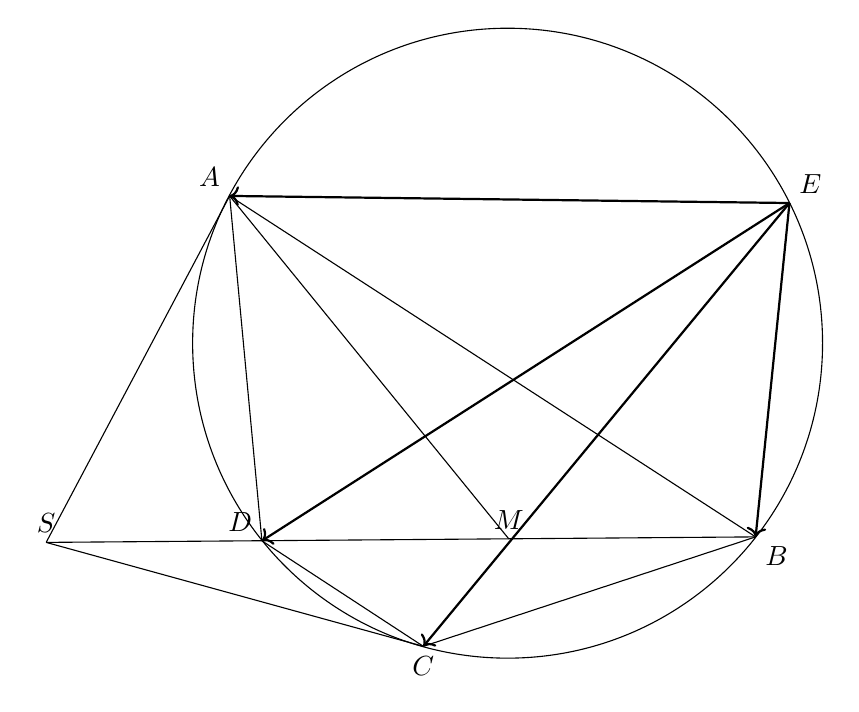
\begin{tikzpicture}
	\draw (-2,2) circle [radius = 4];;
	\draw (-5.53,3.87)node [above left] {$A$}--(1.15,-0.46)node [below 		 	right] {$B$};
	\draw (1.15,-0.46)--(-3.07,-1.85)node [below] {$C$};
	\draw (-3.07,-1.85)--(-5.12,-0.51)node [above left] {$D$};
	\draw (-5.12,-0.51)--(-5.53,3.87);
	\draw (-7.86,-0.53)node [above] {$S$}--(-5.53,3.87);
	\draw (-7.86,-0.53)--(-3.07,-1.85);
	\draw (-7.86,-0.53)--(1.15,-0.46);
	\draw (1.58,3.78)node [above right] {$E$};
	\draw [->] [thick] (1.58,3.78)--(-5.53,3.87);
	\draw [->] [thick] (1.58,3.78)--(1.15,-0.46);
	\draw [->] [thick] (1.58,3.78)--(-3.07,-1.85);
	\draw [->] [thick] (1.58,3.78)--(-5.12,-0.51);
	\draw (-1.985,-0.485)node [above] {$M$};
	\draw (-1.985,-0.485)--(-5.53,3.87);
	\end{tikzpicture}
\end{center}
\(*\left( {a \Leftrightarrow b} \right)\) Lấy \(E\) bất kì trên \(\left( O \right)\). Tứ giác \(ABCD\) là tứ giác điều hòa. \\
\( \Leftrightarrow E\left( {ABCD} \right) =  - 1\) (theo định nghĩa tứ giác điều hòa).\\
\( \Leftrightarrow \frac{{\sin \left( {\overrightarrow {EB} ;\overrightarrow {EA} } \right)}}{{\sin \left( {\overrightarrow {EB} ;\overrightarrow {EC} } \right)}}:\frac{{\sin \left( {\overrightarrow {ED} ;\overrightarrow {EA} } \right)}}{{\sin \left( {\overrightarrow {ED} ;\overrightarrow {EC} } \right)}} =  - 1.\)\\
\( \Leftrightarrow \frac{{BA}}{{BC}} = \frac{{DA}}{{DC}}\) (theo định lí hàm số sin).\\
\( \Leftrightarrow AB.CD = AD.CB.\)\\
\(*\left( {b \Leftrightarrow c} \right)\)\\
\(\left( {c \Rightarrow b} \right)\) Gọi \(S\) là điểm đồng quy của \({\Delta _a}, {\Delta_c}, BD\).\\
Hai tam giác \(SAB\) và \(SDA\) đồng dạng, hai tam giác \(SCB\) và \(SDC\) đồng dạng.\\
Suy ra: \(\frac{{AB}}{{DA}} = \frac{{SA}}{{SD}};\frac{{CB}}{{DC}} = \frac{{SC}}{{SD}}\)\\
Mà \(SA = SC\) \( \Rightarrow \frac{{AB}}{{DA}} = \frac{{CB}}{{DC}} \Rightarrow AB.CD = AD.BC.\)\\
\(\left( {b \Rightarrow c} \right)\) Gọi \(S\) là giao điểm của \({\Delta _a}\) và \({\Delta _c}.\)\\
Gọi \(D'\) là giao điểm của tia \(SB\) và cung $\stackrel\frown{AC}$ (chứa \(D\)) của đường tròn \(\left( O \right)\).\\
Suy ra: \({\Delta _a},{\Delta _c},BD'\) đồng quy tại \(S\). Do đó, theo \(\left( {c \Rightarrow b} \right)\), ta có: \(AB.CD' = AD'.CB\).\\
Mặt khác, do \(AB.CD = AD.BC\) nên \(\frac{{CD'}}{{CD}} = \frac{{AD'}}{{AD}}\), mà \(D\) và \(D'\) cùng thuộc cung $\stackrel\frown{AC}$ (không chứa \(B\)) nên \(\widehat {ADC} = \widehat {AD'C}.\) Do đó, hai tam giác \({ADC}\) và \({AD'C}\) đồng dạng.\\
Từ đó, tương tự như trên, ta có \(D'\) trung với \(D\) nên \(S, B, D\) thẳng hàng.\\
Vậy \({\Delta _a}, {\Delta_c}, BD\) đồng quy. Tương tự với \({\Delta_b}, {\Delta_d}, AC\).\\
\(*\left( {a \Leftrightarrow d} \right)\)\\
Gọi \(P, N\) lần lượt là giao điểm của phân giác các góc \(\widehat {ABC},\widehat {ADC}\) với \(AC\).\\
Tứ giác \(ABCD\) là tứ giác điều hòa.\\
\(\begin{array}{l}
 \Leftrightarrow \frac{{BA}}{{BC}} = \frac{{DA}}{{DC}}.\\
 \Leftrightarrow \frac{{PA}}{{PC}} = \frac{{NA}}{{NC}}.
\end{array}\)\\
\( \Leftrightarrow P \equiv N\) \(\left( {P,N \in AC} \right).\)\\
\(*\left( {a \Leftrightarrow e} \right)\)\\
\(*\left( {e \Rightarrow a} \right)\) Ta có: \(\widehat {MAD} = \widehat {BAC}\) (theo giả thiết), \(\widehat {MDA} = \widehat {BCA}\) (cùng chắn cung $\stackrel\frown{AB}$).\\
\( \Rightarrow \) Hai tam giác \(MAD\) và \(BAC\) đồng dạng \( \Rightarrow \frac{{AD}}{{AC}} = \frac{{MD}}{{BC}}.\)\\
\( \Rightarrow AD.BC = MD.AC = \frac{1}{2}AC.BD.\)\\
Mặt khác, theo định lí Ptolemy, ta có:\\
\(AD.BC + AB.CD = AC.BD.\)\\
\( \Rightarrow AB.CD = \frac{1}{2}AC.BD.\)\\
\( \Rightarrow AB.CD = AD.BC.\)\\
\(\left( {a \Rightarrow e} \right)\) Tứ giác \(ABCD\) là tứ giác điều hòa nên \(AD.BC = AB.CD = \frac{1}{2}BD.AC = MD.AC.\)\\
\( \Rightarrow \frac{{AD}}{{AC}} = \frac{{MD}}{{BC}}.\)\\
Mà \(\widehat {MDA} = \widehat {BCA}\) nên hai tam giác \(MAD\) và \(BAC\) đồng dạng.
\( \Rightarrow \widehat {MAD} = \widehat {BAC}.\)\\
\section{Một vài ví dụ.}
\textbf{Ví dụ 1.} Cho tứ giác \(ABCD\) nội tiếp có hai đường phân giác trong các góc \(\widehat {ABC},\widehat {ADC}\) đồng quy với \(AC\). Gọi \(M\) là trung điểm \(AC\), đường thẳng qua \(D\) và song song với \(BC\) cắt \(BM\) tại \(E\) và cắt đường tròn ngoại tiếp tứ giác \(ABCD\) tại \(F\). Chứng minh rằng tứ giác \(BCEF\) là hình bình hành.\\
\begin{center}
	\begin{tikzpicture}
	\draw (-1,2) circle [radius = 4];
	\draw (-4.786791111576415,3.2884925600428834)-- (1.684179725571905,4.96566673799143);
\draw (1.684179725571905,4.96566673799143)-- (-1.544480861807374,-1.9627693083405067);
\draw (-1.544480861807374,-1.9627693083405067)-- (-4.529232514955346,0.11731100407370398);
\draw (-4.529232514955346,0.11731100407370398)-- (-4.786791111576415,3.2884925600428834);
\draw (1.684179725571905,4.96566673799143)-- (-1.8282929613861927,5.913301773453984);
\draw (-5.056953548765473,-1.0151342728779533)-- (-1.544480861807374,-1.9627693083405067);
\draw (-4.786791111576415,3.2884925600428834)-- (-1.544480861807374,-1.9627693083405067);
\draw (-1.8282929613861927,5.913301773453984)-- (-5.056953548765473,-1.0151342728779533);
\draw (-5.056953548765473,-1.0151342728779533)-- (1.684179725571905,4.96566673799143);
\draw (4.912840312951186,11.894102784323373)-- (-4.786791111576415,3.2884925600428834);
\draw (4.912840312951186,11.894102784323373)-- (-1.544480861807374,-1.9627693083405067);
\draw (-4.6372034142328395,3.6948579124439576) node [above left] 	{$A$};
\draw (1.5198657274283907,5.454020524347174) node {$B$};
\draw (-1.3865768487595191,-1.544387257789537) node [below right] 	{$C$};
\draw (-4.369504755899742,0.48247401244677823) node [below left] 	{$D$};
\draw (-3.011890131496179,1.0369926618510532) node {$M$};
\draw (-4.904902072565936,-0.6456846190998502) node [above left] 	{$E$};
\draw (-1.6733968398306944,6.295359164822626) node {$F$};
\draw (5.195358545258784,12.555449344168343) node {$G$};
	\end{tikzpicture}
\end{center}
\textbf{Lời giải.} Gọi \(G\) là giao điểm của \(AF\) và \(BC\).\\
Từ giả thiết,  hai đường phân giác trong các góc \(\widehat {ABC},\widehat {ADC}\) đồng quy với \(AC\) nên tứ giác \(ABCD\) là tứ giác điều hòa, do đó \(F\left( {ABCD} \right) =  - 1,\) hay \(F\left( {GBCD} \right) =  - 1\).\\
Mà \(FD\) song song với \(GC\) nên \(B\) là trung điểm của \(GC\). \\
Do đó, \(BM\) là đường trung bỉnh của tam giác \(GAC\).
\( \Rightarrow \) \(BM\) song song với \(GA\), mà \(F\left( {ABCD} \right) =  - 1\), hay \(F\left( {GBCE} \right) =  - 1\) nên \(FC\) đi qua trung điểm của \(BE\). \\
Lại có \(BC\) song song với \(EF\) nên tứ giác \(BCEF\) là hình bình hành.\\
\newline
\textbf{Ví dụ 2.} Cho tứ giác \(ABCD\) nội tiếp đường tròn. Gọi \(F, E\) lần lượt là giao điểm của các căp đường thẳng \(AC\) và \(BD\), \(AD\) và \(BC\). Gọi \(M\) là trung điểm \(CD\). \(EF\) cắt đường tròn ngoại tiếp tam giác \(MAB\) tại điểm \(N\) (\(N\) nằm khác phía với \(M\) qua \(AB\)). Chứng minh tứ giác \(NAMB\) là tứ giác điều hòa. \underline{(http://k2pi.net.vn/showthread.php?t=18601)}\\
\begin{center}
	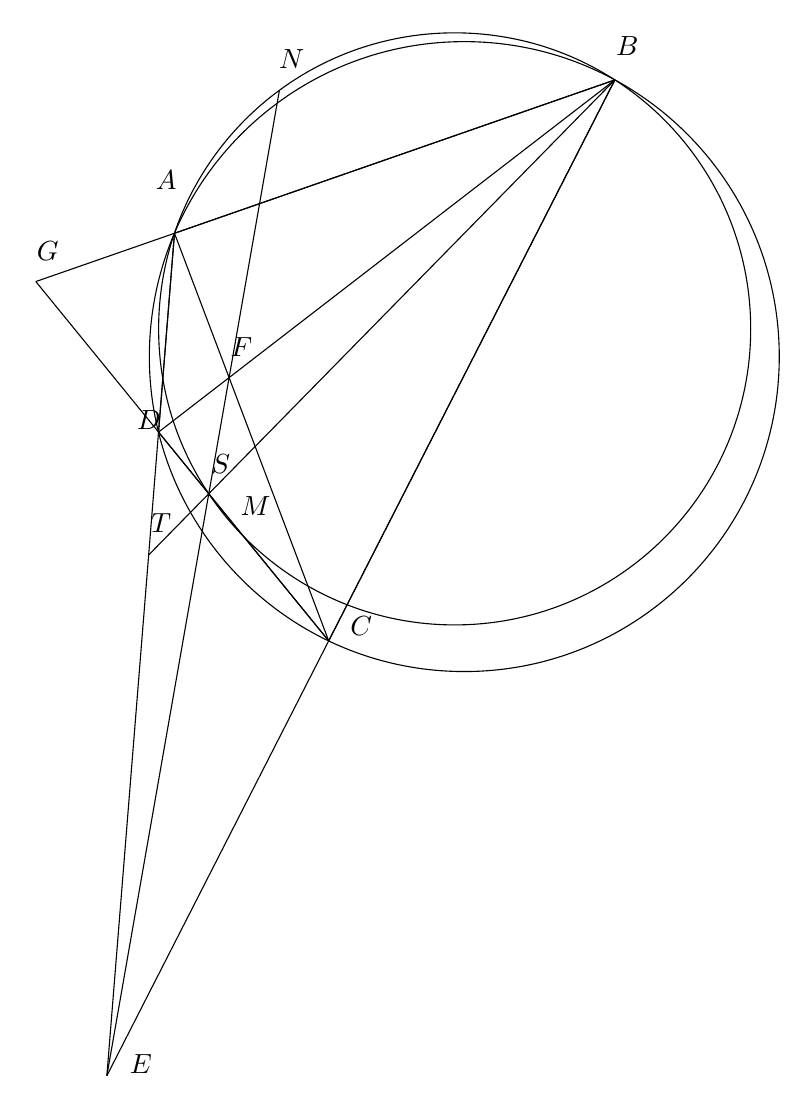
\begin{tikzpicture}
	\draw (-1,2) circle [radius = 4];
\draw (-4.680695002545015,3.5660409631424574)-- (0.9119008964936051,5.513493270519662);
\draw (0.9119008964936051,5.513493270519662)-- (-2.722209881497651,-1.6102621960284056);
\draw (-2.722209881497651,-1.6102621960284056)-- (-4.883378203882584,1.041160219009623);
\draw (-4.883378203882584,1.041160219009623)-- (-4.680695002545015,3.5660409631424574);
\draw (-4.680695002545015,3.5660409631424574)-- (-2.722209881497651,-1.6102621960284056);
\draw (-1.1225373688096725,2.351896672225524) circle [radius = 3.759605312486309];
\draw (-4.883378203882584,1.041160219009623)-- (0.9119008964936051,5.513493270519662);
\draw (-4.680695002545015,3.5660409631424574)-- (-5.539549217436753,-7.132943732613465);
\draw (-5.539549217436753,-7.132943732613465)-- (0.9119008964936051,5.513493270519662);
\draw (0.9119008964936051,5.513493270519662)-- (-6.441599652336171,2.9528591983207706);
\draw (-6.441599652336171,2.9528591983207706)-- (-2.722209881497651,-1.6102621960284056);
\draw (-5.539549217436753,-7.132943732613465)-- (-3.348102884842708,5.381994069920833);
\draw (-5.008663323011488,-0.5195511903592608)-- (0.9119008964936051,5.513493270519662);
\draw (-4.53,4) node [above left] {$A$};
\draw (1.07,5.94) node {$B$};
\draw (-2.57,-1.18) node [below right] {$C$};
\draw (-4.73,1.44) node [below left] {$D$};
\draw (-5.37,-6.74) node [below right] {$E$};
\draw (-3.83,2.12) node {$F$};
\draw (-3.65,0.1) node {$M$};
\draw (-3.19,5.78) node {$N$};
\draw (-6.29,3.34) node {$G$};
\draw (-4.09,0.64) node {$S$};
\draw (-4.85,-0.12) node {$T$};
\end{tikzpicture}
\end{center}
\textbf{Lời giải.} Gọi \(G\) là giao điểm của \(AB\) và \(CD\), \(S\) là giao điểm của \(EF\) và \(CD\).\\
Ta có: \(\left( {GSDC} \right) =  - 1\) (hàng điều hòa tứ giác toàn phần).\\
\(M\) là trung điểm của \(CD\) nên theo công thức Maclaurin, ta có: \(\overline {GS} .\overline {GM}  = \overline {GD} .\overline {GC} \)\\
Mà \(\overline {GD} .\overline {GC}  = \overline {GA} .\overline {GB} \) (phương tích của điểm \(G\) đến đường tròn \(\left( O \right)\)).\\
\( \Rightarrow \overline {GS} .\overline {GM}  = \overline {GA} .\overline {GB} \) \( \Rightarrow \) \(A, B, M, S\) cùng thuộc một đường tròn. \\
Gọi \(T\) là giao điểm của \(SB\) và \(DE\).\\
\( \Rightarrow \left( {TADE} \right) =  - 1\) (hàng điều hòa tứ giác toàn phần \(DECF\).\\
\( \Rightarrow S\left( {TADE} \right) =  - 1 \Rightarrow S\left( {BANM} \right) =  - 1.\)\\
Do đó, tứ giác \(BNAM\) là tứ giác điều hòa.\\
\newline
\textbf{Ví dụ 3.} Cho tam giác \(ABC\) nội tiếp đường tròn \(\left( O \right)\), ngoại tiếp đường tròn \(\left( I \right)\). Gọi \(M\) là tiếp điểm của \(BC\) với \(\left( I \right)\), \(D\) là giao điểm thứ hai của \(AM\) và \(\left( O \right)\). Chứng minh rằng nếu \(OI\) vuông góc với \(AM\) thì tứ giác \(ABDC\) là tứ giác điều hòa. (Đề kiểm tra chọn đội tuyển Ninh Bình)
\begin{center}
	\begin{tikzpicture}
	\draw (4,2) circle [radius = 4];
\draw (1.974549266863309,5.449282436628819)-- (0.12801240733679675,0.9961513648650955);
\draw (0.12801240733679675,0.9961513648650955)-- (6.59794340049406,-1.0414947127735337);
\draw (6.59794340049406,-1.0414947127735337)-- (1.974549266863309,5.449282436628819);
\draw (2.361472246403431,2.037554988178855) circle [radius = 1.6642270529445828];
\draw (1.974549266863309,5.449282436628819)-- (1.8207576777622225,-1.354236560078567);
\draw (4,2)-- (1.8976684459856412,2.0481853520550635);
\draw (-3.607037434561864,2.1724714319846425)-- (3.7169800706157816,3.0030860452928727);
\draw (-3.607037434561864,2.1724714319846425)-- (6.59794340049406,-1.0414947127735337);
\draw (0.12801240733679675,0.9961513648650955)-- (1.7335204787977654,-5.196522625055785);
\draw (1.7335204787977654,-5.196522625055785)-- (6.59794340049406,-1.0414947127735337);
\draw (4.16,2.43) node {$O$};
\draw (2.14,5.87) node {$A$};
\draw (0.52,1.43) node {$B$};
\draw (6.9,-0.65) node {$C$};
\draw (2.52,2.43) node {$I$};
\draw (2.02,0.85) node {$M$};
\draw (1.98,-0.97) node {$D$};
\draw (3.52,0.37) node {$N$};
\draw (2.06,2.43) node {$P$};
\draw (3.88,3.39) node {$E$};
\draw (1.1,2.99) node {$F$};
\draw (-3.44,2.57) node {$S$};
\draw (1.82,-4.49) node {$Q$};
	\end{tikzpicture}
\end{center}
\textbf{Lời giải.} Gọi \(N\) là trung điểm \(BC\); \(E, F\) lần lượt là tiếp điểm của đường tròn \(\left( I \right)\) với \(AC, AB\).\\
Gọi \(S\) là giao điểm của \(EF\) và \(BC\), \(P\) là giao điểm của \(OI\) và \(AM\). \\
\( \Rightarrow \) \(A, F, P, I, E\) cùng thuộc đường tròn đường kính \(AI\).\\
Ta có: \({P_{S/\left( {IM} \right)}} = S{M^2} = \overline {SF} .\overline {SE}  = {P_{S/\left( {IA} \right)}}\) với \(P\) là kí hiệu phương tích từ một điểm đến một đường tròn.\\
\( \Rightarrow \) \(S\) là điểm đẳng phương của đường tròn đường kính \(IM\) và đường tròn đường kính \(AI\).\\
Mà hai đường tròn này cắt nhau tại \(I\) và \(P\) nên \(S, P, I, O\) thẳng hàng.\\
Ta có \(\left( {SMBC} \right) =  - 1\) (hàng điều hòa tứ giác toàn phần \(EFBC\)).\\
\( \Rightarrow \overline {SB} .\overline {SC}  = \overline {SM} .\overline {SN} \) (Maclaurin).\\
\(\overline {SP} .\overline {SO}  = \overline {SM} .\overline {SN} \) (\(M, P, O, N\) đồng viên).
\( \Rightarrow \overline {SB} .\overline {SC}  = \overline {SP} .\overline {SO} \)\\
\( \Rightarrow \) \(B, P, O, C\) đồng viên.\\
Gọi \(Q\) là giao điểm của hai tiếp tuyến tại \(B\) và \(C\) của đường tròn \(\left( O \right)\).\\
\( \Rightarrow \) \(B, P, O, C, Q\) cùng thuộc đường tròn đường kính \(OQ\).\\
\( \Rightarrow \widehat {OPQ} = {90^ \circ }\), mà theo giả thiết ta được \(\widehat {OPQ} = {90^ \circ }\) nên \(A, P, D, Q\) thẳng hàng \( \Rightarrow \) \(BQ, CQ, AD\) đồng quy tại \(Q\).\\
\( \Rightarrow \) Tứ giác \(ABCD\) là tứ giác điều hòa.
\newpage
\textbf{Ví dụ 4.} Cho hình bình hành \(ABCD\), \(M\) là một điểm nằm trên đường chéo \(BD\). \(AM\) cắt \(CD, CB\) lần lượt tại \(K, N\). Gọi \(\left( {{C_1}} \right)\) là đường tròn tâm \(M\), bán kính \(MA\); \(\left( {{C_2}} \right)\) là đường tròn ngoại tiếp tam giác \(KCN\). \(\left( {{C_1}} \right)\) và \(\left( {{C_2}} \right)\) cắt nhau tại \(P, Q\). Chứng minh rằng tứ giác \(PKQN\) là tứ giác điều hòa. (A. Rermerov)\\
\begin{center}
	\begin{tikzpicture}
	\draw (-4,3)--(2,3);
\draw (2,3)--(-1,1);
\draw (-1,1)--(-7,1);
\draw (-7,1)--(-4,3);
\draw (-7,1)--(2,3);
\draw (-1.243176470588235,2.279294117647059) circle [radius=2.8494723969844786];
\draw (1.3251714005876594,-1.068684082672917) circle [radius=3.112213983005517];
\draw (-4,3)--(3.650342801175319,1);
\draw (3.650342801175319,1)--(-1,1);
\draw (-4,3)--(-1,1);
\draw (-3.83,3.42) node {$A$};
\draw (2.17,3.42) node {$B$};
\draw (-1.05,1.44) node {$C$};
\draw (-6.83,1.42) node {$D$};
\draw (-1.09,2.7) node {$M$};
\draw (3.81,1.38) node {$K$};
\draw (0.87,2.16) node {$N$};
\draw (1.75,2.42) node {$P$};
\draw (-1.57,-0.14) node {$Q$};
\draw (-2.33,2.38) node {$O$};
\draw (1.67,1.94) node [below] {$E$};
	\end{tikzpicture}
\end{center}
\textbf{Lời giải.} Gọi \(O\) là trung điểm \(AC\), \(E\) là giao điểm thứ hai của \(AM\) và \(\left( {{C_1}} \right)\).\\
\(MO\) là đường trung bình của tam giác \(CAE\) nên \(CE\) song song với \(BD\).
\( \Rightarrow C\left( {EDOB} \right) =  - 1\) (chùm điều hòa trung tuyến).\\
Hay \(\left( {AEKN} \right) =  - 1.\) \\
\( \Rightarrow M{A^2} = \overline {MK} .\overline {MN} \) (Newton). Lại có \(P, Q\) cùng thuộc đường tròn \(\left( {{C_1}} \right)\) nên \(MA = MP = MQ\) \( \Rightarrow \overline {MK} .\overline {MN}  = M{P^2} = M{Q^2}.\)
\( \Rightarrow \) \(MP, MQ\) là tiếp tuyến của \(\left( {{C_2}} \right)\), do đó tứ giác \(PKQN\) là tứ giác điều hòa.\\
\newpage
\textbf{Ví dụ 5.} Cho tam giác \(ABC\) không cân, \(M\) là trung điểm \(BC\). Đường tròn đường kính \(AM\) lần lượt cắt \(AB, AC, BC\) tại điểm thứ hai \(P, Q, R\). Tiếp tuyến tại \(P, Q\) của đường tròn đường kính \(AM\) cắt nhau tại \(S\). Chứng minh rằng \(SB = SC\).\\
\begin{center}
	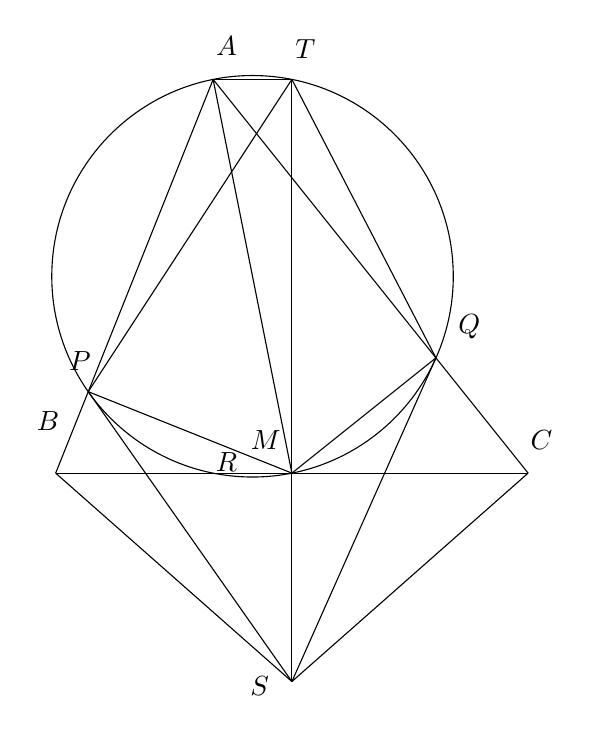
\begin{tikzpicture}
	\draw (-2,4)--(-4,-1);
\draw (-4,-1)--(2,-1);
\draw (2,-1)--(-2,4);
\draw (-2,4)--(-1,-1);
\draw (-1.5,1.5) circle [radius=2.5495097567963922];
\draw (-4,-1)--(-1,-3.6470588235294117);
\draw (-1,-3.6470588235294117)--(2,-1);
\draw (-1,4)--(-1,-3.6470588235294117);
\draw (-1,-3.6470588235294117)--(-3.586206896551724,0.034482758620689884);
\draw (-1,-3.6470588235294117)--(0.8292682926829267,0.46341463414634165);
\draw (-1,4)--(0.8292682926829267,0.46341463414634165);
\draw (0.8292682926829267,0.46341463414634165)--(-1,-1);
\draw (-1,-1)--(-3.586206896551724,0.034482758620689884);
\draw (-3.586206896551724,0.034482758620689884)--(-1,4);
\draw (-2,4)--(-1,4);
\draw (-1.83,4.42) node {$A$};
\draw (-3.83,-0.58) node [above left] {$B$};
\draw (2.17,-0.58) node {$C$};
\draw (-1.33,-0.58) node {$M$};
\draw (-3.43,0.42) node [left] {$P$};
\draw (0.99,0.86) node [right] {$Q$};
\draw (-1.83,-0.62) node [below] {$R$};
\draw (-1.41,-3.46) node [below] {$S$};
\draw (-0.83,4.38) node {$T$};
	\end{tikzpicture}
\end{center}
\textbf{Lời giải.} Gọi \(T\) là giao điểm thứ hai của \(SM\) với đường tròn đường kính \(AM\). Khi đó, ta có tứ giác \(TPMQ\) là tứ giác điều hòa.\\
Điểm \(A\) nằm trên đường tròn ngoại tiếp tứ giác \(TPMQ\) nên \(A\left( {TMPQ} \right) =  - 1.\)\\
\( \Rightarrow A\left( {TMBC} \right) =  - 1\).
Mà \(M\) là trung điểm \(BC\) nên chùm \(A\left( {TMBC} \right)\) là chùm trung tuyến, do đó \(AT\) song song với \(BC\).\\
Lại có \(AT \bot TM\) hay \(AT \bot SM\) (do \(T\) thuộc đường tròn đường kính \(AM\)).\\
\( \Rightarrow SM \bot BC\) tại trung điểm \(M\) của \(BC\) nên \(SM\) là đường trung trực của \(BC\).\\
Vậy \(SB = SC\).\\
\textbf{Nhận xét:} Bài toán trên là một bài toán khá đơn giản, ta hoàn toàn có thể nhìn ra điểm \(T\) một cách dễ dàng. Dù vậy, kết luận của bài toán này thực sự rất thú vị, nó xuất hiện trong nhiều bài toán khác như sau:\\
\textbf{Ví dụ 5.1.} Cho tam giác \(ABC\) có \(M, N, P\) lần lượt là trung điểm của \(AB, AC, BC\). Kẻ \(BI\) vuông góc với \(MP\) tại \(I\), \(CK\) vuông góc với \(NP\) tại \(K\). Tiếp tuyến tại \(I, K\) của đường tròn ngoại tiếp tam giác \(IKP\) cắt nhau tại \(T\). Chứng minh rằng \(TB = TC\). (VMO 2014).\\
\textbf{Ví dụ 5.2.} Cho tứ giác \(ABCD\) nội tiếp đường tròn \(\left( O \right)\). Kẻ \(OM\) vuông góc với \(AD\) \(\left( {M \in AC} \right)\), \(ON\) vuông góc với \(BC\) \(\left( {N \in BD} \right).\) Tiếp tuyến tại \(M\) và \(N\) của đường tròn ngoại tiếp tam giác \(OMN\) cắt nhau tại \(S\). Chứng minh rằng \(SB = SC\).\\
\newpage
\textbf{Ví dụ 6.} Cho tam giác \(ABC\), \(M, N\) lần lượt nằm trên \(AB, AC\) sao cho \(MN\) song song với \(BC\). Gọi \(P\) là giao điểm của \(CM\) và \(BN\). Đường tròn ngoại tiếp hai tam giác \(MBP\) và \(NPC\) cắt nhau tại điểm thứ hai \(Q\)) . Chứng minh rằng \(\widehat {BAQ} = \widehat {PAC}.\)
\begin{center}
	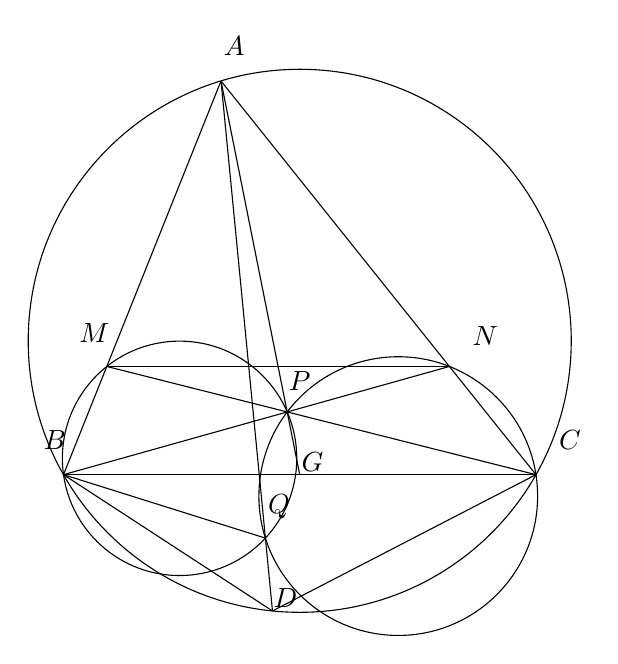
\begin{tikzpicture}
	\draw (-2,4)--(-4,-1);
\draw (-4,-1)--(2,-1);
\draw (2,-1)--(-2,4);
\draw (-4,-1)--(0.900689655172414,0.37413793103448256);
\draw (2,-1)--(-3.450344827586207,0.37413793103448256);
\draw (-2.526152475181558,-0.7925390099273772) circle [radius=1.4883771661831426];
\draw (0.2513248889746612,-1.2721469853719953) circle [radius=1.769725579169422];
\draw (-2,4)--(-1.4360013262599467,-1.8058687002652523);
\draw (-2,4)--(-1,-1);
\draw (-1,0.7) circle [radius=3.448187929913333];
\draw (-4,-1)--(-1.3461538461538458,-2.73076923076923);
\draw (-1.3461538461538458,-2.73076923076923)--(2,-1);
\draw (-4,-1)--(-1.4360013262599467,-1.8058687002652523);
\draw (-1.4360013262599467,-1.8058687002652523)--(-1.3461538461538458,-2.73076923076923);
\draw (-3.450344827586207,0.37413793103448256)--(0.900689655172414,0.37413793103448256);
\draw (-1.8323330471083827,4.439526375162066) node {$A$};
\draw (-3.843592286411753,-0.5581480982584288) node [left] {$B$};
\draw(2.1698696816064054,-0.5581480982584288) node [right] {$C$};
\draw (-3.2950670393290156,0.8030071445024376) node [left] {$M$};
\draw (1.0728191874409303,0.7623756447185313) node [right] {$N$};
\draw (-0.9993873015382999,0.19353464774384077) node {$P$};
\draw (-1.263492050133692,-1.4114095937204645) node {$Q$};
\draw (-0.836861302402674,-0.5987795980423352) node [below] {$G$};
\draw (-1.182229050565879,-2.32561833885836) node [below] {$D$};
	\end{tikzpicture}
\end{center}
\textbf{Lời giải.} Gọi \(G\) là giao điểm của \(AP\) và \(BC\), \(AQ\) cắt đường tròn \(\left( {ABC} \right)\) tại điểm thứ hai \(D\).\\
Theo định lí Ceva, ta được \(G\) là trung điểm của \(BC\).\\
Xét mod \(\pi \): \(\left( {BQ,BM} \right) \equiv \left( {PQ,PC} \right) \equiv \left( {NQ,NC} \right).\)\\
\(\Rightarrow\) \(B, A, N, Q\) đồng viên \( \Rightarrow \widehat {BQD} = \widehat {BNC}.\)\\
\(\Rightarrow\) Hai tam giác \(BQD\) và \(BNC\) đồng dạng \( \Rightarrow \frac{{BD}}{{BC}} = \frac{{QD}}{{NC}}.\)\\
Tương tự: \(\frac{{CD}}{{BC}} = \frac{{QD}}{{MB}}\). Khi đó: \(\frac{{BD}}{{CD}} = \frac{{MB}}{{NC}} = \frac{{AB}}{{AC}}.\)\\
Do đó, tứ giác \(ABDC\) là tứ giác điều hòa. \\
\(G\) là trung điểm \(BC\) nên \(\widehat {BAD} = \widehat {GAC}\), suy ra đpcm.\\
\textbf{Nhận xét:} Đây là một bài toán hay và lạ. Bài toán không hề nhắc đến tứ giác điều hòa hay các tính chất của nó, tuy vậy ta vẫn có thể nhìn ra \(G\) là trung điểm \(BC\) cộng với yêu cầu của đề bài để tìm cách chứng minh \(AQ\) là đường đối trung của tam giác \(ABC\), hay \(ABCD\) là tứ giác điều hòa. Sau đây xin gửi đến bạn đọc một bài toán tương tự, cũng khá hay và đẹp:
\textbf{Ví dụ 6.1.} Cho tam giác \(ABC\) nội tiếp đường tròn \(\left( O \right)\) và một điểm \(P\) nằm bên trong tam giác. \(AP, BP, CP\) lần lượt cắt \(BC, CA, AB\) tại \(D, E, F\). Tiếp tuyến tại \(A\) của đường tròn \(\left( O \right)\), \(EF, BC\) đồng quy tại \(S\). Đường tròn ngoại tiếp tam giác \(SAD\) cắt đường tròn \(\left( O \right)\) tại điểm thứ hai \(G\). \(GE, GF\) lần lượt cắt \(\left( O \right)\) tại điểm thứ hai \(M, N\). \(CN\) cắt \(DM\) tại \(I\). Chứng minh rằng \(\widehat {ABD} = \widehat {IAC}\).
\newpage
\textbf{Ví dụ 7.} Cho đường tròn \(\left( O \right)\) đường kính \(AB\). Trên tiếp tuyến tại \(A\) của \(\left( O \right)\), lấy điểm \(M\) khác \(A\). Từ \(M\), kẻ cát tuyến \(MCD\) đến đường tròn \(\left( O \right)\). \(MO\) cắt \(BC, BD\) lần lượt tại \(X, Y\). Chứng minh rằng \(OX = OY\).
\begin{center}
	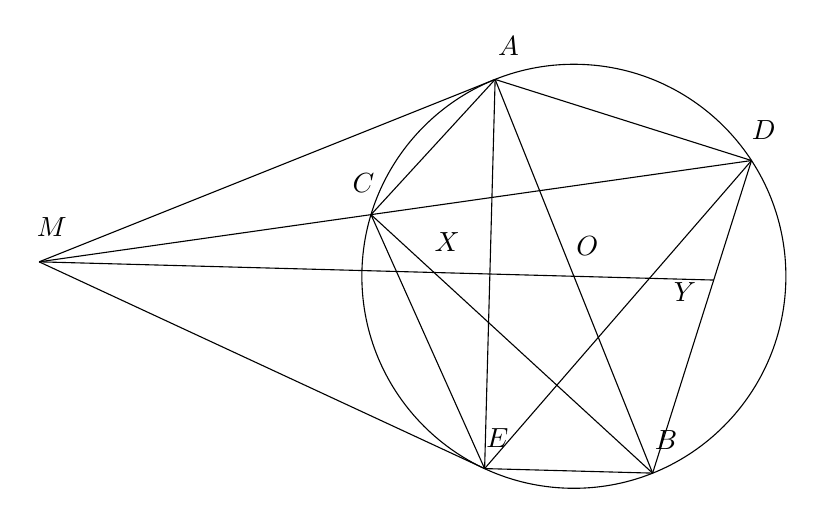
\begin{tikzpicture}
	\draw (-3,4)--(-1,-1);
\draw (-2,1.5) circle [radius=2.692582403567252];
\draw (-8.791379310344828,1.6834482758620686)--(-3,4);
\draw (-8.791379310344828,1.6834482758620686)--(0.2560911391146048,2.9697117989621518);
\draw (-1,-1)--(-4.5763123049252155,2.282697200385263);
\draw (-1,-1)--(0.2560911391146048,2.9697117989621518);
\draw (-8.791379310344828,1.6834482758620686)--(-0.22413168226454203,1.4520303658271);
\draw (-8.791379310344828,1.6834482758620686)--(-3.1335029611783183,-0.9423699631710146);
\draw (-3,4)--(-4.5763123049252155,2.282697200385263);
\draw (-4.5763123049252155,2.282697200385263)--(-3.1335029611783183,-0.9423699631710146);
\draw (-3.1335029611783183,-0.9423699631710146)--(0.2560911391146048,2.9697117989621518);
\draw (0.2560911391146048,2.9697117989621518)--(-3,4);
\draw (-3.1335029611783183,-0.9423699631710146)--(-1,-1);
\draw (-3,4)--(-3.1335029611783183,-0.9423699631710146);
\draw (-2.83,4.42) node {$A$};
\draw (-0.83,-0.58) node {$B$};
\draw (-1.83,1.88) node {$O$};
\draw (-8.63,2.12) node {$M$};
\draw (-4.41,2.68) node [left] {$C$};
\draw (0.41,3.36) node {$D$};
\draw (-3.61,1.94) node {$X$};
\draw (-0.59,1.3) node {$Y$};
\draw (-2.97,-0.56) node {$E$};
	\end{tikzpicture}
\end{center}
\textbf{Lời giải.} Gọi \(ME\) là tiếp tuyến thứ hai từ \(M\) đến \(\left( O \right)\) (\(E\) là tiếp điểm).\\
Ta được tứ giác \(ACED\) là tứ giác điều hòa.\\
\( \Rightarrow B\left( {AECD} \right) =  - 1\) hay \(B\left( {OEXY} \right) =  - 1.\)\\
Mà \(MO\) song song với \(BE\) do cùng vuông góc với \(AE\) nên \(OX = OY\) (chùm điều hòa trung tuyến).\\
\textbf{Nhận xét:} Thực sự rất ấn tượng với lời giải ngắn gọn bằng tứ giác điều hòa của bài toán. Nếu giải bằng kiến thức Trung học Cơ sở, ta sẽ phải xét hai trường hợp với lời giải khá rắc rối cùng hình phụ. Bài toán trên đồng thời cũng là một bổ đề hay được sử dụng nhiều trong các kết quả đẹp khác, chẳng hạn như:\\
\textbf{Ví dụ 7.1.} Từ một điểm \(M\) ở ngoài đường tròn \(\left( O \right)\), kẻ tiếp tuyến \(MA\), cát tuyến \(MBC\) đến đường tròn. \(D, E\) lần lượt là điểm đối xứng với \(C, A\) qua \(O\). .Chứng minh rằng \(EB, DA, MO\) đồng quy.
\begin{center}
	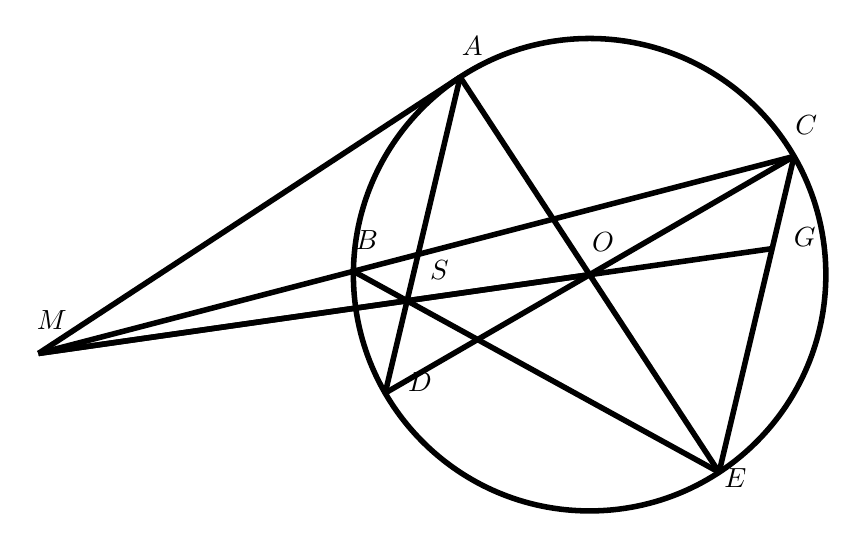
\begin{tikzpicture}
	\draw [line width=2pt] (-2,2) circle (3cm);
\draw [line width=2pt] (-0.3558125457540289,-0.5093121797217961)-- (-4.999685525956368,2.0434366822843026);
\draw [line width=2pt] (-4.596293069310363,0.49691573814008283)-- (-3.644187454245971,4.509312179721796);
\draw [line width=2pt] (-9,1)-- (-2,2);
\draw [line width=2pt] (-9,1)-- (-3.644187454245971,4.509312179721796);
\draw [line width=2pt] (-9,1)-- (0.5962930693103634,3.503084261859917);
\draw [line width=2pt] (0.5962930693103634,3.503084261859917)-- (-0.3558125457540289,-0.5093121797217961);
\draw [line width=2pt] (-3.644187454245971,4.509312179721796)-- (-0.3558125457540289,-0.5093121797217961);
\draw [line width=2pt] (-4.596293069310363,0.49691573814008283)-- (0.5962930693103634,3.503084261859917);
\draw [line width=2pt] (-9,1)-- (0.31820899106312506,2.331172713009018);
\draw (-1.83,2.42) node {$O$};
\draw (-8.83,1.42) node {$M$};
\draw (-3.49,4.9) node {$A$};
\draw (-4.83,2.44) node {$B$};
\draw (0.75,3.9) node {$C$};
\draw (-4.43,0.88) node [below right] {$D$};
\draw (-0.15,-0.58) node {$E$};
\draw (0.47,2.72) node [ below right] {$G$};
\draw (-4.15,2.06) node [right] {$S$};
	\end{tikzpicture}
\end{center}
\textbf{Gợi ý.} Gọi \(G, S\) lần lượt là giao điểm của \(MO\) với \(EC, EB\).\\
Theo ví dụ 7, ta có \(O\) là trung điểm \(GS\) \( \Rightarrow \) \(DS\) song song với \(EC\).\\
Mà tứ giác \(DACE\) là hình chữ nhật nên \(DA\) song song với \(CE\). Do đó, \(D, S, A\) thẳng hàng.\\
\textbf{Ví dụ 7.2} Cho tam giác \(ABC\) nội tiếp đường tròn \(\left( O \right)\) có phân giác \(AD\). Dây cung \(PQ\) bất kì của \(\left( O \right)\) song song với \(BC\). \(PD, QD\) lần lượt cắt \(\left( O \right)\) tại điểm thứ hai \(X, Y\). \(G\) là điểm đối xứng với \(A\) qua \(O\). \(XY\) cắt \(BC\) tại \(M\), \(GX\) cắt \(MO\) tại \(H\), \(GY\) cắt \(MO\) tại \(K\). Chứng minh rằng \(O\) là trung điểm của \(HK\).
\begin{center}
	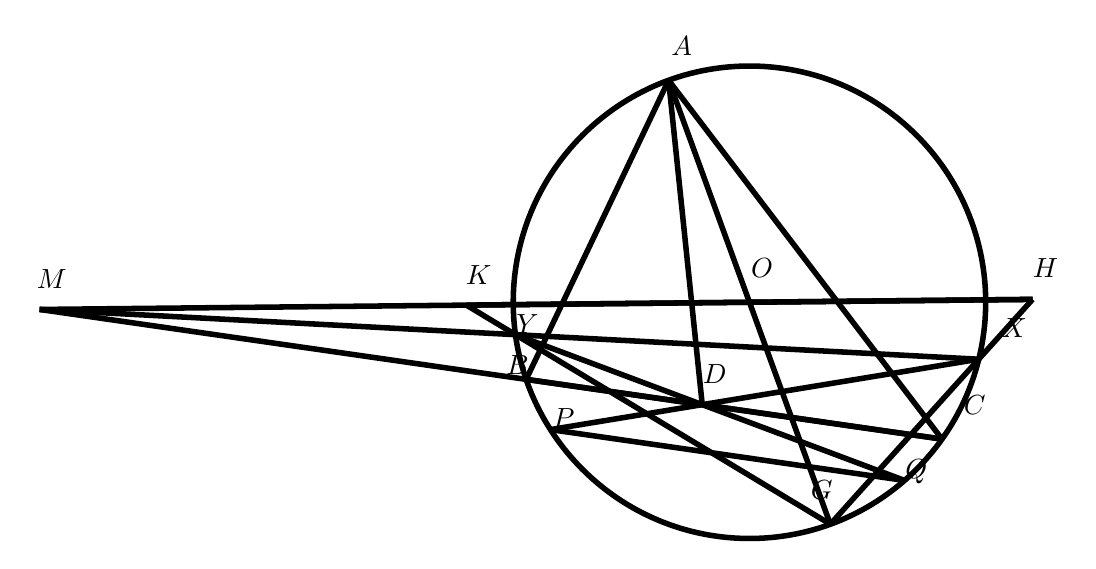
\begin{tikzpicture}
	\draw [line width=2pt] (-2,2) circle (3cm);
\draw [line width=2pt] (-3.026845637583893,4.818791946308725)-- (-4.835685071828252,1.0207706226780144);
\draw [line width=2pt] (-4.835685071828252,1.0207706226780144)-- (0.44529009790873797,0.26202521966817005);
\draw [line width=2pt] (0.44529009790873797,0.26202521966817005)-- (-3.026845637583893,4.818791946308725);
\draw [line width=2pt] (-3.026845637583893,4.818791946308725)-- (-0.973154362416107,-0.8187919463087248);
\draw [line width=2pt] (-5.594965952707814,1.9635744954663605)-- (1.5949659527078155,2.036425504533639);
\draw [line width=2pt] (-4.526814201984534,0.3828389107298984)-- (-0.030689428310152197,-0.2631429190907508);
\draw [line width=2pt] (-4.526814201984534,0.3828389107298984)-- (0.9114507016762089,1.2764982296434162);
\draw [line width=2pt] (-0.030689428310152197,-0.2631429190907508)-- (-4.971618230678742,1.5883143297396205);
\draw [line width=2pt] (0.9114507016762089,1.2764982296434162)-- (-11.01546503124018,1.9086520243339298);
\draw [line width=2pt] (-11.01546503124018,1.9086520243339298)-- (0.44529009790873797,0.26202521966817005);
\draw [line width=2pt] (-0.973154362416107,-0.8187919463087248)-- (1.5949659527078155,2.036425504533639);
\draw [line width=2pt] (-0.973154362416107,-0.8187919463087248)-- (-5.594965952707814,1.9635744954663605);
\draw [line width=2pt] (-11.01546503124018,1.9086520243339298)-- (1.5949659527078155,2.036425504533639);
\draw [line width=2pt] (-3.026845637583893,4.818791946308725)-- (-2.5997092798627697,0.6995162522508952);
\draw (-1.84,2.43) node {$O$};
\draw (-2.86,5.25) node {$A$};
\draw (-4.68,1.45) node [below left] {$B$};
\draw (0.6,0.69) node [right] {$C$};
\draw (-2.44,1.09) node {$D$};
\draw (-4.36,0.77) node [below] {$P$};
\draw (0.12,0.13) node [below] {$Q$};
\draw (1.08,1.67) node [right] {$X$};
\draw (-4.82,1.97) node [below] {$Y$};
\draw (-0.82,-0.39) node [left] {$G$};
\draw(-10.86,2.29) node {$M$};
\draw (1.76,2.43) node {$H$};
\draw (-5.44,2.35) node {$K$};
	\end{tikzpicture}
\end{center}
\textbf{Gợi ý.} Tiếp tuyến tại \(A\) của đường tròn \(\left( O \right)\) cắt \(BC\) tại \(M'\).\\
Ta có: \(A{{M'}^2} = \overline {M'B} .\overline {M'C} \), mà \(AM' = DM'\) nên \(D{{M'}^2} = \overline {M'B} .\overline {M'C} \).\\
Lại có hai tam giác \(MDY\) và \(MXD\) đồng dạng nên \(M{D^2} = \overline {MX} .\overline {MY}  = \overline {MB} .\overline {MC} \).\\
Vậy \(M' \equiv M\), dẫn đến đpcm.\\
\textbf{Nhận xét:} Hai bài toán trên nếu không biết cách đưa về bổ đề quen thuộc thì sẽ dẫn đến thế khó, cả hai bài đều có sự phức tạp về hình vẽ, khó suy đoán hướng làm, thế nhưng nếu biết cách tận dụng yếu tố tứ giác điều hòa để giải quyết thì vấn đề sẽ trở nên đơn giản.\\
\newline
\textbf{Ví dụ 8.} Cho tứ giác \(ABCD\) nội tiếp đường tròn \(\left( O \right)\), \(AC\) cắt \(BD\) tại \(M\). Đường thẳng qua \(M\) và vuông góc với \(MO\) cắt \(BC\) tại \(P\), \(DP\) cắt \(\left( O \right)\) tại điểm thứ hai \(S\). Lấy điểm \(Q\) nằm trên \(\left( O \right)\) sao cho \(DQ\) vuông góc với \(OM\). TIa phân giác các góc \(\widehat {ABS},\widehat {AQS}\) cắt nhau tại \(R\). Tiếp tuyến tại \(B, Q\) của \(\left( O \right)\) cắt nhau tại \(T\). Chứng minh rằng \(A, R, S, T\) thẳng hàng.\\
\textbf{Lời giải.}
\textbf{Bổ đề:} Cho đường tròn \(\left( O \right)\) với dây cung \(AB\). Gọi \(I\) là trung điểm của \(AB\), qua \(I\) dựng hai dây cung \(MN, PQ\) sao cho \(MP, NQ\) cắt \(AB\) lần lượt tại \(E, F\). Chứng minh rằng \(I\) là trung điểm của \(EF\).
\begin{center}
	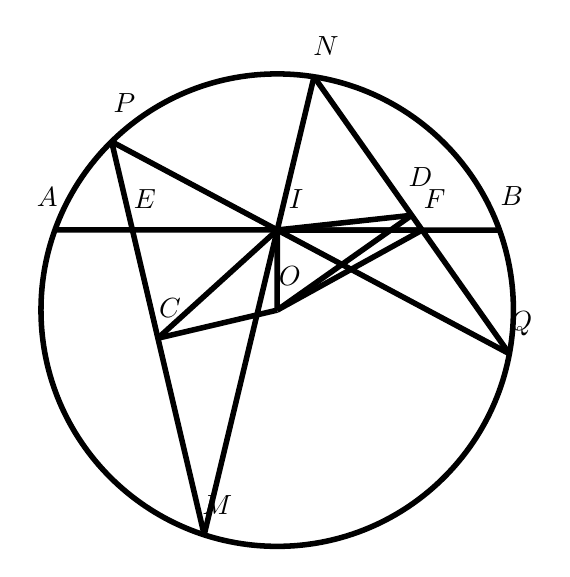
\begin{tikzpicture}
	\draw [line width=2pt] (4,2) circle (3cm);
\draw [line width=2pt] (1.178871322748484,3.0204082449633143)-- (6.8229210378474665,3.01543922224729);
\draw [line width=2pt] (4,2)-- (2.4850001842945133,1.6433182311625663);
\draw [line width=2pt] (4,2)-- (5.707887943958493,3.204729528997322);
\draw [line width=2pt] (4.000896180297975,3.0179237336053024)-- (4,2);
\draw [line width=2pt] (4.000896180297975,3.0179237336053024)-- (5.84080178285569,3.0163038802737496);
\draw [line width=2pt] (4.000896180297975,3.0179237336053024)-- (5.707887943958493,3.204729528997322);
\draw [line width=2pt] (4,2)-- (5.84080178285569,3.0163038802737496);
\draw [line width=2pt] (4.000896180297975,3.0179237336053024)-- (2.4850001842945133,1.6433182311625663);
\draw [line width=2pt] (1.8972591262035121,4.139738492822332)-- (3.072741242385514,-0.853102030497199);
\draw [line width=2pt] (3.072741242385514,-0.853102030497199)-- (4.467356044850927,4.963372795876566);
\draw [line width=2pt] (4.467356044850927,4.963372795876566)-- (6.948419843066058,1.4460862621180781);
\draw [line width=2pt] (6.948419843066058,1.4460862621180781)-- (1.8972591262035121,4.139738492822332);
\draw (4.16,2.43) node {$O$};
\draw (1.08,3.43) node {$A$};
\draw (6.98,3.45) node {$B$};
\draw (4.24,3.41) node {$I$};
\draw (3.24,-0.47) node {$M$};
\draw (4.62,5.35) node {$N$};
\draw (2.06,4.63) node {$P$};
\draw (7.1,1.83) node {$Q$};
\draw (2.32,3.41) node {$E$};
\draw (6,3.41) node {$F$};
\draw (2.64,2.03) node {$C$};
\draw (5.82,3.69) node {$D$};
	\end{tikzpicture}
\end{center}
Vì \(I\) là trung điểm của \(AB\) nên \(OI \bot AB.\)\\
Gọi \(C, D\) lần lượt là trung điểm của \(MP, NQ\) \( \Rightarrow OC \bot MP\) và \(OD \bot NQ\).\\
Vậy các tứ giác \(IOCE, IODF\) là tứ giác nội tiếp.\\
\( \Rightarrow \widehat {IOE} = \widehat {ICE}\) và \(\widehat {IOF} = \widehat {IDF}\).\\
Mặt khác, hai tam giác \(IMP\) và \(IQN\) đồng dạng và \(IC, ID\) là hai đường trung tuyến tương ứng \( \Rightarrow \frac{{IC}}{{ID}} = \frac{{IP}}{{IN}} = \frac{{PM}}{{NQ}} = \frac{{CP}}{{DN}}.\) Do đó, hai tam giác \(ICP\) và \(IDN\) đồng dạng. Từ đó, ta có: \(\widehat {ICE} = \widehat {IDF}.\) \\
Do đó: \(\widehat {IOE} = \widehat {IOF}\) \( \Rightarrow \) tam giác \(OEF\) cân tại \(O\) \( \Rightarrow \) \(I\) là trung điểm \(EF\).\\
\textbf{Quay lại bài toán:} 
\begin{center}
	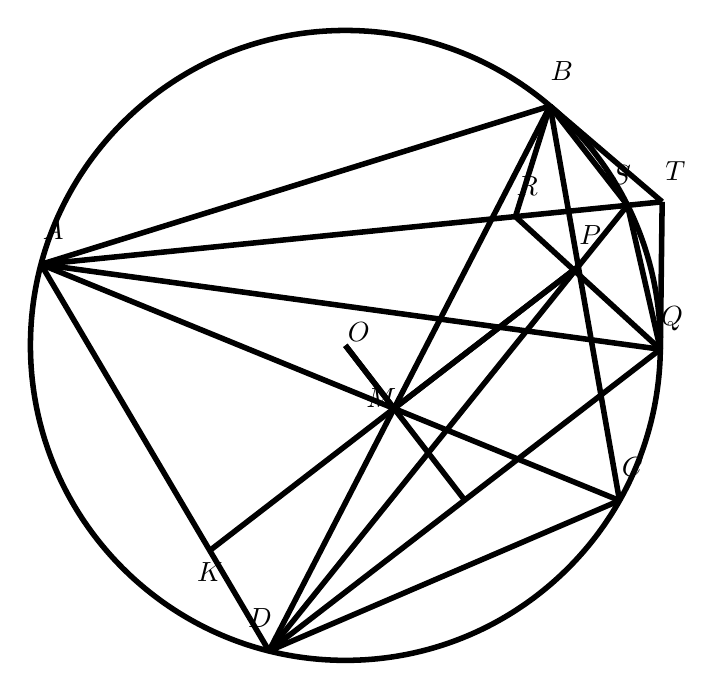
\begin{tikzpicture}
	\draw [line width=2pt] (-2,2) circle (4cm);
\draw [line width=2pt] (-5.865436646601809,3.0287854640826524)-- (0.599031079596668,5.040565317057106);
\draw [line width=2pt] (0.599031079596668,5.040565317057106)-- (1.4811099882756102,0.029752997838144335);
\draw [line width=2pt] (1.4811099882756102,0.029752997838144335)-- (-2.970142500145332,-1.8805700005813275);
\draw [line width=2pt] (-2.970142500145332,-1.8805700005813275)-- (-5.865436646601809,3.0287854640826524);
\draw [line width=2pt] (-5.865436646601809,3.0287854640826524)-- (1.4811099882756102,0.029752997838144335);
\draw [line width=2pt] (-2.970142500145332,-1.8805700005813275)-- (0.599031079596668,5.040565317057106);
\draw [line width=2pt] (-2,2)-- (-1.3822226566946776,1.1986324715157703);
\draw [line width=2pt] (-1.3822226566946776,1.1986324715157703)-- (0.9577918005317896,3.002558714217107);
\draw [line width=2pt] (-2.970142500145332,-1.8805700005813275)-- (1.5825172888326289,3.7792048435228898);
\draw [line width=2pt] (-2,2)-- (-0.4852231741740759,0.035063968803776255);
\draw [line width=2pt] (-2.970142500145332,-1.8805700005813275)-- (1.9996961517971803,1.95069793818888);
\draw [line width=2pt] (0.599031079596668,5.040565317057106)-- (1.5825172888326289,3.7792048435228898);
\draw [line width=2pt] (1.5825172888326289,3.7792048435228898)-- (1.9996961517971803,1.95069793818888);
\draw [line width=2pt] (-5.865436646601809,3.0287854640826524)-- (1.9996961517971803,1.95069793818888);
\draw [line width=2pt] (1.9996961517971803,1.95069793818888)-- (0.159209077569641,3.63579927550955);
\draw [line width=2pt] (0.159209077569641,3.63579927550955)-- (0.599031079596668,5.040565317057106);
\draw [line width=2pt] (-5.865436646601809,3.0287854640826524)-- (2.022781942004779,3.8235637548006682);
\draw [line width=2pt] (2.022781942004779,3.8235637548006682)-- (1.9996961517971803,1.95069793818888);
\draw [line width=2pt] (2.022781942004779,3.8235637548006682)-- (0.599031079596668,5.040565317057106);
\draw [line width=2pt] (0.9577918005317896,3.002558714217107)-- (-3.722237113921145,-0.6052937711855664)node [below] {$K$};;
\draw (-1.83,2.42) node [below] {$O$};
\draw (-5.71,3.46) node {$A$};
\draw (0.75,5.48) node {$B$};
\draw (1.65,0.46) node {$C$};
\draw (-2.81,-1.46) node [left] {$D$};
\draw (-1.23,1.58) node [below left] {$M$};
\draw (1.11,3.4) node {$P$};
\draw (1.75,4.16) node [left] {$S$};
\draw (2.15,2.34) node {$Q$};
\draw (0.31,4.02) node {$R$};
\draw (2.19,4.22) node {$T$};
	\end{tikzpicture}
\end{center}
Gọi \(K\) là giao điểm của \(PM\) và \(AD\).
Theo bổ đề, ta có \(M\) là trung điểm của \(PK\). Mà \(DQ\) song song với \(PK\) nên \(D\left( {KPMQ} \right) =  - 1\), hay \(D\left( {ASPQ} \right) =  - 1.\) \\
\( \Rightarrow \) Tứ giác \(APQS\) là tứ giác điều hòa.
\( \Rightarrow \) Tiếp tuyến tại \(B, Q\) của đường tròn \(\left( O \right)\) đồng quy với \(AS\).\\
Tương tự như trên, ta có tứ giác \(ABSQ\) là tứ giác điều hòa nên đường phân giác hai góc \(\widehat {ABS},\widehat {AQS}\) cắt nhau tại một điểm trên \(AS\). Do đó, \(A, R, S, T\) thẳng hàng.\\
\newpage
\textbf{Ví dụ 9.} Cho hai đường tròn \(\left( {{O_1}} \right),\left( {{O_2}} \right)\) tiếp xúc ngoài tại \(A\). Từ một điểm \(M\) trên \(\left( {{O_2}} \right)\) nhưng không thuộc \({O_1}{O_2}\), kẻ hai tiếp tuyến \(MB, MC\) tới \(\left( {{O_1}} \right)\). \(AB, AC\) cắt \(\left( {{O_2}} \right)\) tại điểm thứ hai \(D, E\). \(DE\) và tiếp tuyến tại \(M\) của đường tròn \(\left( {{O_2}} \right)\)  cắt nhau tại \(N\). Chứng minh rằng \(N\) luôn nằm trên đường thẳng cố định khi \(M\) thay đổi. (VMO 2003)\\
\begin{center}
	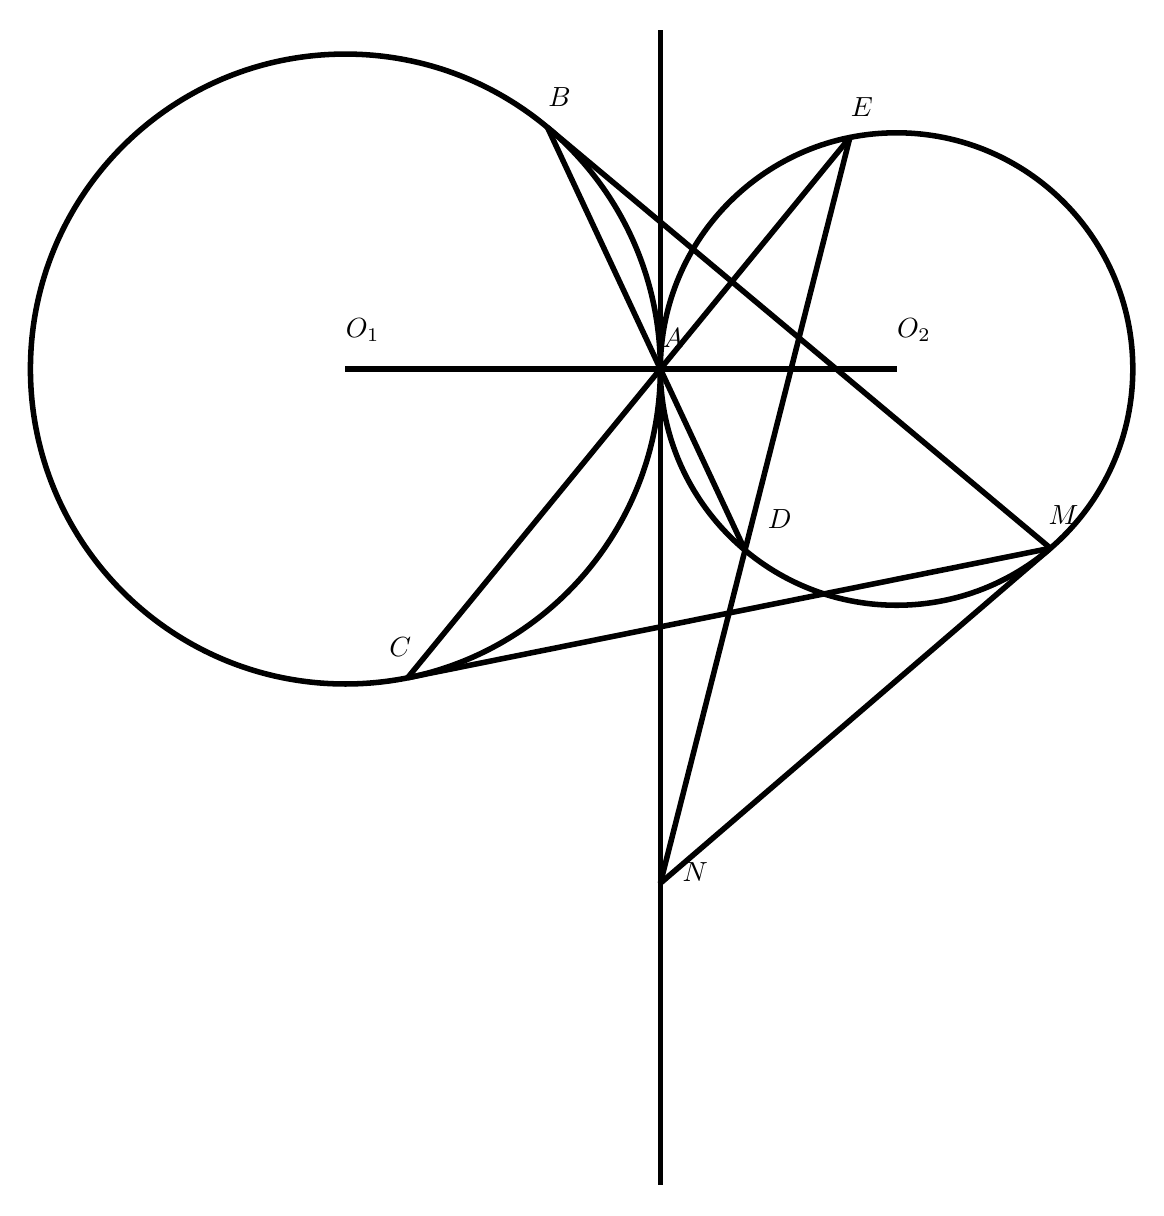
\begin{tikzpicture}
	\draw [line width=2pt] (-2,2) circle (4cm);
\draw [line width=2pt] (5,2) circle (3cm);
\draw [line width=2pt] (0.5666391124607006,5.067957572455484)-- (6.954410699743274,-0.27602258704280036);
\draw [line width=2pt] (6.954410699743274,-0.27602258704280036)-- (-1.2098529280724137,-1.9211819142605795);
\draw [line width=2pt] (-2,2)-- (5,2);
\draw [line width=2pt] (2,-8.36) -- (2,6.3);
\draw [line width=2pt] (0.5666391124607006,5.067957572455484)-- (3.0750206656544745,-0.300968179341613);
\draw [line width=2pt] (-1.2098529280724137,-1.9211819142605795)-- (4.40738969605431,4.940886435695435);
\draw [line width=2pt] (6.954410699743274,-0.27602258704280036)-- (2,-4.5303535139962685);
\draw [line width=2pt] (4.40738969605431,4.940886435695435)-- (2,-4.5303535139962685);
\draw (-1.78,2.49) node {$O_1$};
\draw (5.22,2.49) node {$O_2$};
\draw (2.16,2.39) node {$A$};
\draw (7.12,0.15) node {$M$};
\draw (0.72,5.45) node {$B$};
\draw (-1.04,-1.53) node [left] {$C$};
\draw (3.24,0.09) node [right] {$D$};
\draw (4.56,5.33) node {$E$};
\draw (2.16,-4.15) node [below right] {$N$};
	\end{tikzpicture}
\end{center}
\textbf{Lời giải.} Ta có hai tam giác \({O_1}AB\) và \({O_2}AD\) đồng dạng với nhau nên \(\widehat {A{O_1}B} = \widehat {A{O_2}D}.\)\\
Tương tự: \(\widehat {A{O_1}C} = \widehat {A{O_2}E}.\)\\
\( \Rightarrow \frac{{\overline {EC} }}{{\overline {DB} }} = \frac{{\overline {EA} }}{{\overline {DA} }}\).\\
Mà \(\widehat {MBA} = \frac{1}{2}\widehat {A{O_1}B} = \frac{1}{2}\widehat {A{O_2}D} = \widehat {AMD}.\) nên hai tam giác \(AMD\) và \(MBD\) đồng dạng.\\
\( \Rightarrow D{M^2} = \overline {DA} .\overline {DB} \). Tương tự: \(E{M^2} = \overline {EA} .\overline {EC} .\)\\
\( \Rightarrow \frac{{D{M^2}}}{{E{M^2}}} = \frac{{\overline {DA} .\overline {DB} }}{{\overline {EA} .\overline {EC} }} = \frac{{D{A^2}}}{{E{A^2}}} \Rightarrow \frac{{DM}}{{EM}} = \frac{{DA}}{{EA}}.\)\\
\( \Rightarrow \) Tứ giác \(AEMD\) là tứ giác điều hòa.\\
Mặt khác, \(N\) là giao điểm của \(DE\) và tiếp tuyến tại \(M\) của  \(\left( {{O_2}} \right)\) nên \(N\) thuộc tiếp tuyến chung tại \(A\) của hai đường tròn. Đường thẳng này cố định nên ta có đpcm.\\
\textbf{Nhận xét:} Đây là một bài toán khá hay và lời giải sử dụng tứ giác điều hòa khá đẹp mắt, ngoài cách giải bằng tứ giác điều hòa, ta có thể chứng minh bài toán bằng cách sử dụng phương tích, trục đẳng phương, chứng minh \(N\) là điểm đẳng phương của hai đường tròn \(\left( {{O_1}} \right),\left( {{O_2}} \right)\) và đường tròn điểm \(M\). Sau đây là một số bài toán về quỹ tích chứng minh bằng tính chất của tứ giác điều hòa.\\
\textbf{Ví dụ 9.1.} (Vietnam TST 2001) Trong mặt phẳng cho hai đường tròn \({\omega _1},{\omega _2}\) có tâm lần lượt là \({O_1},{O_2}\) cắt nhau tại hai điể \(A, B\). Các tiếp tuyến tại \(A, B\) của \({\omega _1}\) cắt nhau tại \(K\). Giả sử \(M\) là một điểm nằm trên \({\omega _1}\) nhưng không trùng với \(A, B\). Đường thẳng \(AM\) cắt \({\omega _2}\) tại điểm thứ hai \(P\), đường thẳng \(KM\) cắt \({\omega _1}\) tại điểm thứ hai \(C\) và đường thẳng \(AC\) cắt \({\omega _2}\) tại điểm thứ hai \(Q\).\\
a. Chứng minh rằng trung điểm của đoạn thẳng \(PQ\) nằm trên đường thẳng \(MC\).\\
b. Chứng minh rằng đường thẳng \(PQ\) luôn đi qua một điểm cố định khi \(M\) di chuyển trên \({\omega _1}\). \\
\textbf{Ví dụ 9.2} Từ một điểm \(M\) nằm ngoài \(\left( O \right)\) kẻ hai tiếp tuyến \(MB, MC\) đến đường tròn. \(A\) là một điểm cố định trên \(\left( O \right)\). Đường thẳng bất kì qua \(A\) cắt \(\left( O \right)\) tại \(G\), cắt \(MB, MC\) lần lượt tại \(D, E\), \(BE\) cắt \(CD\) tại \(S\). Chứng minh rằng \(GS\) luôn đi qua một điểm cố định. \\
\newline
\textbf{Ví dụ 10.} Đường tròn \(\left( I \right)\) nội tiếp tam giác \(ABC\) lần lượt tiếp xúc \(BC, CA, AB\) tại \(D, E, F\). \(AD\) cắt \(\left( I \right)\) tại điểm thứ hai \(P\). Cho rằng \(\widehat {BPC} = {90^ \circ }\), chứng minh rằng \(EA + AP = PD\). (China 2003)\\
\begin{center}
	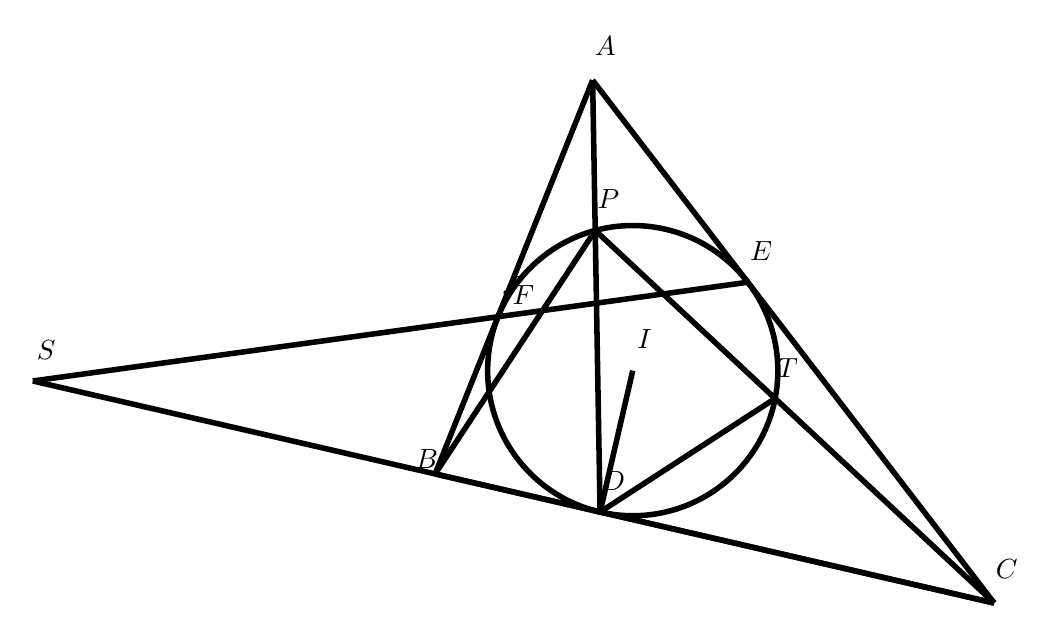
\begin{tikzpicture}
	\draw [line width=2pt] (-4,-2)-- (3.1,-3.64);
\draw [line width=2pt] (-1.4906433032076118,-0.6883578683445023) circle (1.842747543678488cm);
\draw [line width=2pt] (-2,3)-- (-4,-2);
\draw [line width=2pt] (3.1,-3.64)-- (-2,3);
\draw [line width=2pt] (-2,3)-- (-1.9053719782388632,-2.4838295712236995);
\draw [line width=2pt] (-4,-2)-- (-1.9670713272122484,1.091736187506519);
\draw [line width=2pt] (-1.9670713272122484,1.091736187506519)-- (3.1,-3.64);
\draw [line width=2pt] (0.31785665255035545,-1.041976900293478)-- (-1.9053719782388632,-2.4838295712236995);
\draw [line width=2pt] (-0.029219588454309886,0.4341211896738468)-- (-9.109298233328783,-0.8198240700479995);
\draw [line width=2pt] (-9.109298233328783,-0.8198240700479995)-- (3.1,-3.64);
\draw [line width=2pt] (-1.4906433032076118,-0.6883578683445023)-- (-1.9053719782388632,-2.4838295712236995);
\draw (3.26,-3.21) node {$C$};
\draw (-3.84,-1.57) node [below left] {$B$};
\draw (-1.84,3.43) node {$A$};
\draw (-1.34,-0.29) node {$I$};
\draw (-1.74,-2.09) node {$D$};
\draw (0.14,0.83) node {$E$};
\draw (-2.88,0.27) node {$F$};
\draw (-3.04,0.39) node {$J$};
\draw (-1.8,1.49) node {$P$};
\draw (-8.94,-0.43) node {$S$};
\draw (0.48,-0.65) node {$T$};
	\end{tikzpicture}
\end{center}
\textbf{Lời giải.} Gọi \(S\) là giao điểm của \(EF\) và \(BC\), \(T\) là giao điểm thứ hai của \(BC\) và \(\left( I \right)\).\\
Ta có: \(P\left( {BCDE} \right) =  - 1\), mà \(BP \bot PC\) \( \Rightarrow \) \(PC\) là tia phân giác của góc \(\widehat {DPS}\).\\
\( \Rightarrow \widehat {DPC} = \widehat {CPS} = \widehat {PDT}\).\\
\( \Rightarrow \) \(PT = DT\).\\
Lại có tứ giác \(PETD\) là tứ giác điều hòa nên \(PT.DE = 2PE.DT\) (định lí Ptolemy).\\
Mà \(PT = DT\) nên \(DE = 2PE\).\\
Mặt khác, hai tam giác \(AEP\) và \(ADE\) đồng dạng \\
\( \Rightarrow \) \(AD = 2AE\) và \(AE = 2AP\) suy ra: \(PD = EA + AP\).\\
\textbf{Nhận xét:} Đây là một bài toán hay, làm nổi bật tính chất của tứ giác điều hòa và định lí Ptolemy, vốn có quan hệ sâu sắc với nhau. Chìa khóa để giải bài toán này nằm ở việc tạo ra tứ giác \(PETD\) là tứ giác điều hòa và sử dụng các tính chất quen thuộc để suy ra các quan hệ độ dài. Mối liên kết giữa định lí Ptolemy và tứ giác điều hòa còn được thể hiện qua các bài toán sau:\\
\textbf{Ví dụ 10.1.} Cho tam giác \(ABC\) ngoại tiếp đường tròn \(\left( I \right)\), các tiếp điểm với \(BC, CA, AB\) lần lượt là \(D, E, F\). \(BE, CF\) lần lượt cắt \(\left( I \right)\) tại điểm thứ hai \(R, T\). Chứng minh rằng \(EF, BC, RT\) đồng quy.
\begin{center}
	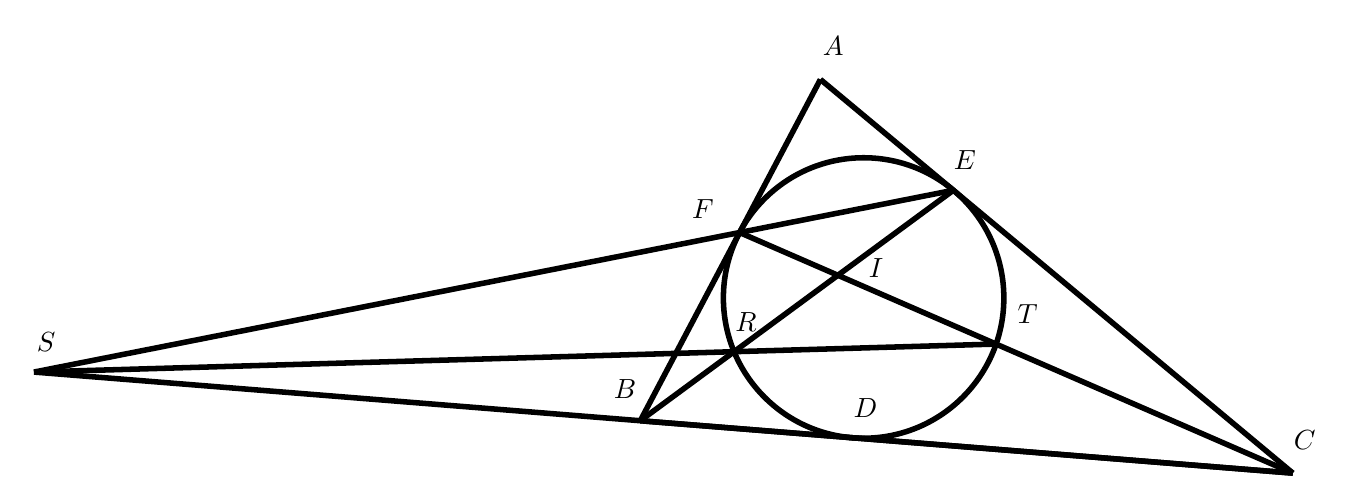
\begin{tikzpicture}
	\draw [line width=2pt] (-2,4)-- (-4.2875928276882105,-0.33463183115098816);
\draw [line width=2pt] (-4.2875928276882105,-0.33463183115098816)-- (4,-1);
\draw [line width=2pt] (4,-1)-- (-2,4);
\draw [line width=2pt] (-1.4511136391809414,1.2243201593565105) circle (1.7809478335468116cm);
\draw [line width=2pt] (-4.2875928276882105,-0.33463183115098816)-- (-0.31097861952801964,2.5924821829400164);
\draw [line width=2pt] (4,-1)-- (-3.0261761769612203,2.0555560993255613);
\draw [line width=2pt] (-0.31097861952801964,2.5924821829400164)-- (-11.987191417528528,0.2835293069636503);
\draw [line width=2pt] (-11.987191417528528,0.2835293069636503)-- (4,-1);
\draw [line width=2pt] (-11.987191417528528,0.2835293069636503)-- (0.2309355914181061,0.6390974909163396);
\draw (-1.8373539338812936,4.419998403260056) node {$A$};
\draw (-4.482056231958601,0.06401814760331198) node {$B$};
\draw (4.1521189176467255,-0.5777110864889762) node {$C$};
\draw (-1.292856401924201,1.6002790413393957) node {$I$};
\draw (-1.4289807849134744,-0.16933793752115642) node {$D$};
\draw (-0.1649686571559379,2.9809692116591675) node {$E$};
\draw (-3.4902928701796103,2.3586863179939184) node {$F$};
\draw (-2.945795338222518,0.9196571263930295) node {$R$};
\draw (0.3795288748011547,1.0168888285282247) node [right] {$T$};
\draw (-11.832772913379351,0.6668547008415221) node {$S$};
	\end{tikzpicture}
\end{center}
\textbf{Lời giải.} Gọi \(S, S'\) lần lượt là giao điểm của \(EF\) với \(BC, RT\).\\
Ta có: \(\frac{{\overline {SE} }}{{\overline {SF} }} = \frac{{D{E^2}}}{{D{F^2}}},\frac{{\overline {S'E} }}{{\overline {S'F} }} = \frac{{RE}}{{RF}}.\frac{{TE}}{{TF}}.\)\\
Theo định lí Ptolemy:\\
Tứ giác \(EFRD\) là tứ giác điều hòa \( \Rightarrow \frac{{RE}}{{RF}} = 2\frac{{DE}}{{DF}}.\)\\
Tứ giác \(EFDT\) là tứ giác điều hòa \( \Rightarrow \frac{{TE}}{{TF}} = \frac{{DE}}{{2DF}}.\)\\
\( \Rightarrow \frac{{\overline {SE} }}{{\overline {SF} }} = \frac{{\overline {S'E} }}{{\overline {S'F} }}\) \( \Rightarrow S \equiv S'.\)\\
Vậy ta có đpcm.\\
\textbf{Nhận xét:} Bản chất của bài toán trên chính là một bổ đề quen thuộc: Từ \(M\) ở ngoài đường tròn \(\left( O \right)\) kẻ hai cát tuyến \(MAB, MCD\), hai tiếp tuyến \(MP, MQ\) đến đường tròn. Chứng minh rằng \(PQ, AD, BC\) đồng quy.\\
\newline
\textbf{Ví dụ 10.2.} Cho tam giác \(ABC\) ngoại tiếp đường tròn \(\left( I \right)\), các tiếp điểm với \(BC, CA, AB\) lần lượt là \(D, E, F\). \(AD, CF\) lần lượt cắt đường tròn \(\left( I \right)\) tại điểm thứ hai \(H, K\). Chứng minh rằng \(\frac{{FD.HK}}{{FH.DK}} = 3.\)\\
\begin{center}
	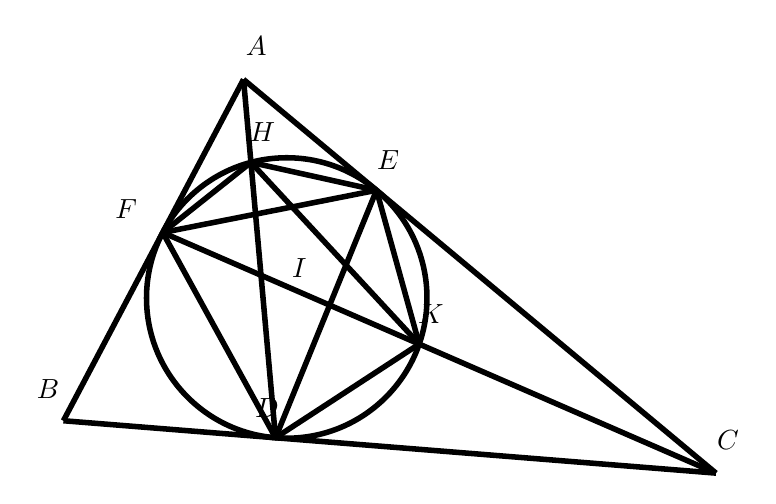
\begin{tikzpicture}
	\draw [line width=2pt] (-2,4)-- (-4.2875928276882105,-0.33463183115098816);
\draw [line width=2pt] (-4.2875928276882105,-0.33463183115098816)-- (4,-1);
\draw [line width=2pt] (4,-1)-- (-2,4);
\draw [line width=2pt] (-1.4511136391809414,1.2243201593565105) circle (1.7809478335468116cm);
\draw [line width=2pt] (4,-1)-- (-3.0261761769612203,2.0555560993255613);
\draw [line width=2pt] (-2,4)-- (-1.5936381791525718,-0.5509155831072775);
\draw [line width=2pt] (-3.0261761769612203,2.0555560993255613)-- (-1.5936381791525718,-0.5509155831072775);
\draw [line width=2pt] (-1.9059055481593514,2.9462201289664924)-- (0.2309355914181061,0.6390974909163396);
\draw [line width=2pt] (-1.9059055481593514,2.9462201289664924)-- (-3.0261761769612203,2.0555560993255613);
\draw [line width=2pt] (0.2309355914181061,0.6390974909163396)-- (-1.5936381791525718,-0.5509155831072775);
\draw [line width=2pt] (-1.9059055481593514,2.9462201289664924)-- (-0.31097861952801964,2.5924821829400164);
\draw [line width=2pt] (-0.31097861952801964,2.5924821829400164)-- (-1.5936381791525718,-0.5509155831072775);
\draw [line width=2pt] (-3.0261761769612203,2.0555560993255613)-- (-0.31097861952801964,2.5924821829400164);
\draw [line width=2pt] (-0.31097861952801964,2.5924821829400164)-- (0.2309355914181061,0.6390974909163396);
\draw (-1.8373539338812936,4.419998403260056) node {$A$};
\draw (-4.482056231958601,0.06401814760331198) node {$B$};
\draw (4.1521189176467255,-0.5777110864889762) node {$C$};
\draw (-1.292856401924201,1.6002790413393957) node {$I$};
\draw (-1.4289807849134744,-0.16933793752115642) node [left] {$D$};
\draw (-0.1649686571559379,2.9809692116591675) node {$E$};
\draw (-3.4902928701796103,2.3586863179939184) node {$F$};
\draw (-1.7595685721731376,3.33100333934587) node {$H$};
\draw (0.3795288748011547,1.0168888285282247) node {$K$};
	\end{tikzpicture}
\end{center}
\textbf{Lời giải.} Theo định lí Ptolemy:\\
Tứ giác \(FHED\) là tứ giác điều hòa \( \Rightarrow \) \(ED.FK = 2FE.DK\).\\
Tứ giác \(FEKD\) là tứ giác điều hòa \( \Rightarrow \) \(HD.FE = 2HF.DE\).\\
Nhân vế theo vế của hai đẳng thức trên, ta được: \(FK.HD = 4DK.HF\).\\
Mà \(FH.DK + FD.HK = FK.HD\).\\
Từ hai điều trên, ta có: \(FD.HK=3FH.DK\) (đpcm).\\
\textbf{Nhận xét:} Bài toán trên cho ta gợi ý về tính chất của các cặp tứ giác điều hòa có chung ba đỉnh, cụ thể trong lời giải trên là \(FHED\) và \(FEKD\). Mời bạn đọc đến với một kết quả đẹp sau đây phát triển từ ví dụ trên:\\
\textbf{Ví dụ 10.3.} Cho tam giác \(ABC\) ngoại tiếp đường tròn \(\left( I \right)\), các tiếp điểm với \(BC, CA, AB\) lần lượt là \(D, E, F\). \(AD\) cắt đường tròn \(\left( I \right)\) tại điểm thứ hai \(M\). Đường tròn ngoại tiếp tam giác \(MCD\) cắt \(DF\) tại điểm thứ hai \(N\). \(CN\) cắt \(AB\) tại \(G\). Chứng minh \(CD = 3FG\).\\
\begin{center}
	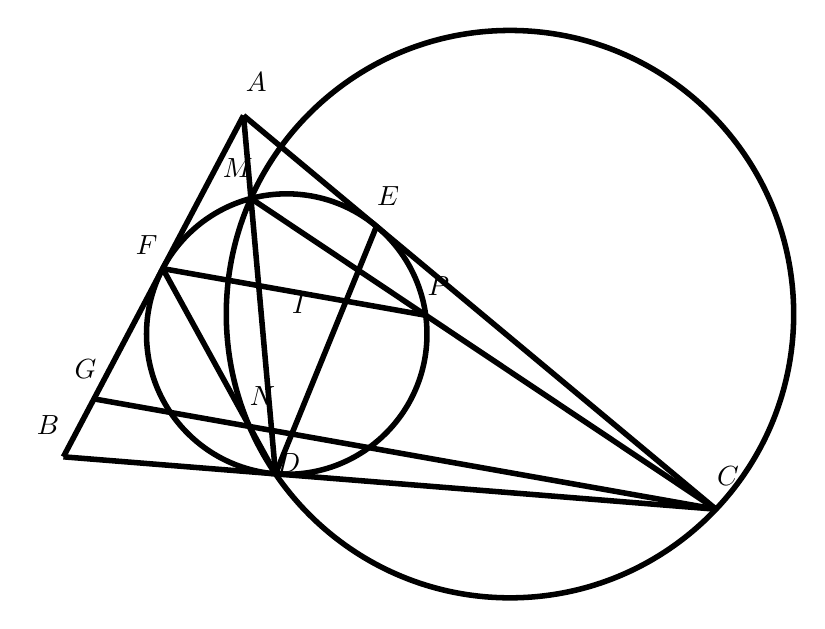
\begin{tikzpicture}
	\draw [line width=2pt] (-2,4)-- (-4.2875928276882105,-0.33463183115098816);
\draw [line width=2pt] (-4.2875928276882105,-0.33463183115098816)-- (4,-1);
\draw [line width=2pt] (4,-1)-- (-2,4);
\draw [line width=2pt] (-1.4511136391809414,1.2243201593565105) circle (1.7809478335468116cm);
\draw [line width=2pt] (-2,4)-- (-1.5936381791525718,-0.5509155831072775);
\draw [line width=2pt] (-3.0261761769612203,2.0555560993255613)-- (-1.5936381791525718,-0.5509155831072775);
\draw [line width=2pt] (-0.31097861952801964,2.5924821829400164)-- (-1.5936381791525718,-0.5509155831072775);
\draw [line width=2pt] (1.3840576236111353,1.4774791854300848) circle (3.602923483898366cm);
\draw [line width=2pt] (-3.8992307575398324,0.40125375604857655)-- (4,-1);
\draw [line width=2pt] (-1.9059055481593514,2.9462201289664924)-- (4,-1);
\draw [line width=2pt] (-3.0261761769612203,2.0555560993255613)-- (0.3137569579112099,1.4630814655488569);
\draw (-1.8373539338812936,4.419998403260056) node {$A$};
\draw (-4.482056231958601,0.06401814760331198) node {$B$};
\draw (4.1521189176467255,-0.5777110864889762) node {$C$};
\draw (-1.292856401924201,1.6002790413393957) node {$I$};
\draw (-1.4289807849134744,-0.16933793752115642) node [below] {$D$};
\draw (-0.1649686571559379,2.9809692116591675) node {$E$};
\draw (-3.4902928701796103,2.3586863179939184) node [right] {$F$};
\draw (-1.7595685721731376,3.33100333934587) node [left] {$M$};
\draw (-1.7595685721731376,0.43349861571705367) node {$N$};
\draw(-3.743095295731118,0.7835327434037563) node [left] {$G$};
\draw (0.4767605769363498,1.8336351264638642) node {$P$};
	\end{tikzpicture}
\end{center} 
\textbf{Lời giải.} Gọi \(P\) là giao điểm thứ hai của \(MC\) và đường tròn \(\left( I \right)\). Ta có \(FP\) song song với \(CG\).\\
\( \Rightarrow \frac{{FG}}{{CD}} = \frac{{FG}}{{CP}}.\frac{{CP}}{{CD}} = \frac{{\sin \widehat {PCG}}}{{\sin \widehat {FGC}}}.\frac{{\sin \widehat {PDC}}}{{\sin \widehat {DPC}}} = \frac{{\sin \widehat {DFP}}}{{\sin \widehat {FDP}}}.\frac{{\sin \widehat {FDM}}}{{\sin \widehat {DFM}}} = \frac{{PD}}{{PF}}.\frac{{MF}}{{MD}}.\)\\
Theo định lí Ptolemy:\\
Tứ giác \(FMED\) là tứ giác điều hòa \( \Rightarrow \) \(FM.ED = ME.FD\).\\
Tứ giác \(PEMD\) là tứ giác điều hòa \( \Rightarrow \) \(2EM.PD = MP.ED\).\\
Nhân vế theo vế hai đẳng thức trên, ta có: \(2FM.DP = FD.MP\).\\
Mà \(FM.DP + FD.MP = FP.MD\).\\
\( \Rightarrow \) \(3FM.DP = FP.DM\). \( \Rightarrow \) \(\frac{{FG}}{{CD}} = \frac{1}{3}.\) (đpcm)\\
\\
\textbf{Ví dụ 11.} Cho tam giác \(ABC\) ngoại tiếp đường tròn \(\left( I \right)\), các tiếp điểm với \(BC, CA, AB\) lần lượt là \(D, E, F\). \(AD\) cắt \(\left( I \right)\) tại điểm thứ hai \(X\). \(BX, CX\) theo thứ tự cắt \(\left( I \right)\) tại điểm thứ hai \(Y, Z\). \(AY, AZ\) lần lượt cắt \(\left( I \right)\) tại điểm thứ hai \(R, S\). Chứng minh rằng \(AD, ES, FR\) đồng quy.\\
\begin{center}
	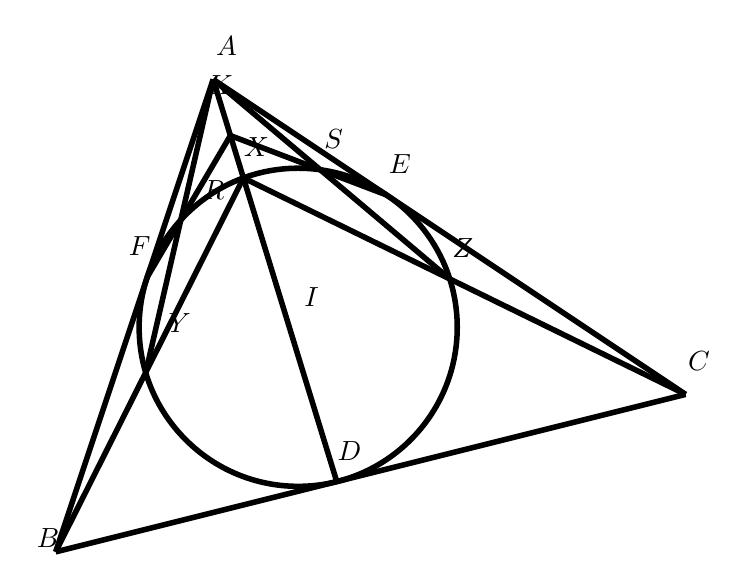
\begin{tikzpicture}
	\draw [line width=2pt] (-2,4)-- (-4,-2);
\draw [line width=2pt] (-4,-2)-- (4,0);
\draw [line width=2pt] (4,0)-- (-2,4);
\draw [line width=2pt] (-0.9199674881957767,0.8522060158698974) circle (2.0200286647829144cm);
\draw [line width=2pt] (-2,4)-- (-0.43003857339134344,-1.107509643347836);
\draw [line width=2pt] (-1.6153891355452572,2.7487567109324833)-- (-4,-2);
\draw [line width=2pt] (-1.6153891355452572,2.7487567109324833)-- (4,0);
\draw [line width=2pt] (-2,4)-- (-2.8564529478194256,0.2772800456695339);
\draw [line width=2pt] (-2,4)-- (1.004443683287734,1.466337475424043);
\draw [line width=2pt] (-1.7808508713672968,3.287048542179363)-- (-2.8363349440586085,1.4909951678241748);
\draw [line width=2pt] (-1.7808508713672968,3.287048542179363)-- (0.20054280853989423,2.5329714609734038);
\draw (-1.83,4.42) node {$A$};
\draw (-3.83,-1.58) node [below left] {$B$};
\draw (4.17,0.42) node {$C$};
\draw(-0.75,1.24) node {$I$};
\draw (-0.27,-0.72) node {$D$};
\draw (0.37,2.92) node {$E$};
\draw (-2.67,1.88) node [left] {$F$};
\draw (-1.45,3.14) node {$X$};
\draw (-2.69,0.66) node [above right] {$Y$};
\draw (1.17,1.86) node {$Z$};
\draw (-2.25,2.6) node [right] {$R$};
\draw (-0.47,3.24) node {$S$};
\draw(-1.63,3.68) node [above left] {$K$};
	\end{tikzpicture}
\end{center}
\textbf{Lời giải.} Gọi \(K\) là giao điểm của \(ES\) và \(AD\).\\
Tứ giác \(ZEXD\) là tứ giác điều hòa và \(S\) là một điểm thuộc đường tròn ngoại tiếp tứ giác \(ZEXD\) nên \(S\left( {ZEXD} \right) =  - 1.\)\\
\( \Rightarrow \left( {AXKD} \right) = S\left( {AXKD} \right) = S\left( {ZEXD} \right) =  - 1.\)\\
Gọi \(K'\) là giao điểm của \(FR\) và \(AD\). Tương tự như trên, ta được \(\left( {AXK'D} \right)  = -1\).\\
\( \Rightarrow K \equiv K'.\) Vậy \(AD, ES, FR\) đồng quy.\\
\newline
\textbf{Ví dụ 12.} (IMO 2002) Cho tam giác \(ABC\) ngoại tiếp đường tròn \(\left( I \right)\), các tiếp điểm với \(BC, CA, AB\) lần lượt là \(D, E, F\). Gọi \(G\) là trung điểm của đường cao \(AH\). \(DG\) cắt \(\left( I \right)\) tại điểm thứ hai \(T\). Chứng minh rằng đường tròn ngoại tiếp tam giác \(TBC\) tiếp xúc với đường tròn \(\left( I \right)\).\\
\begin{center}
	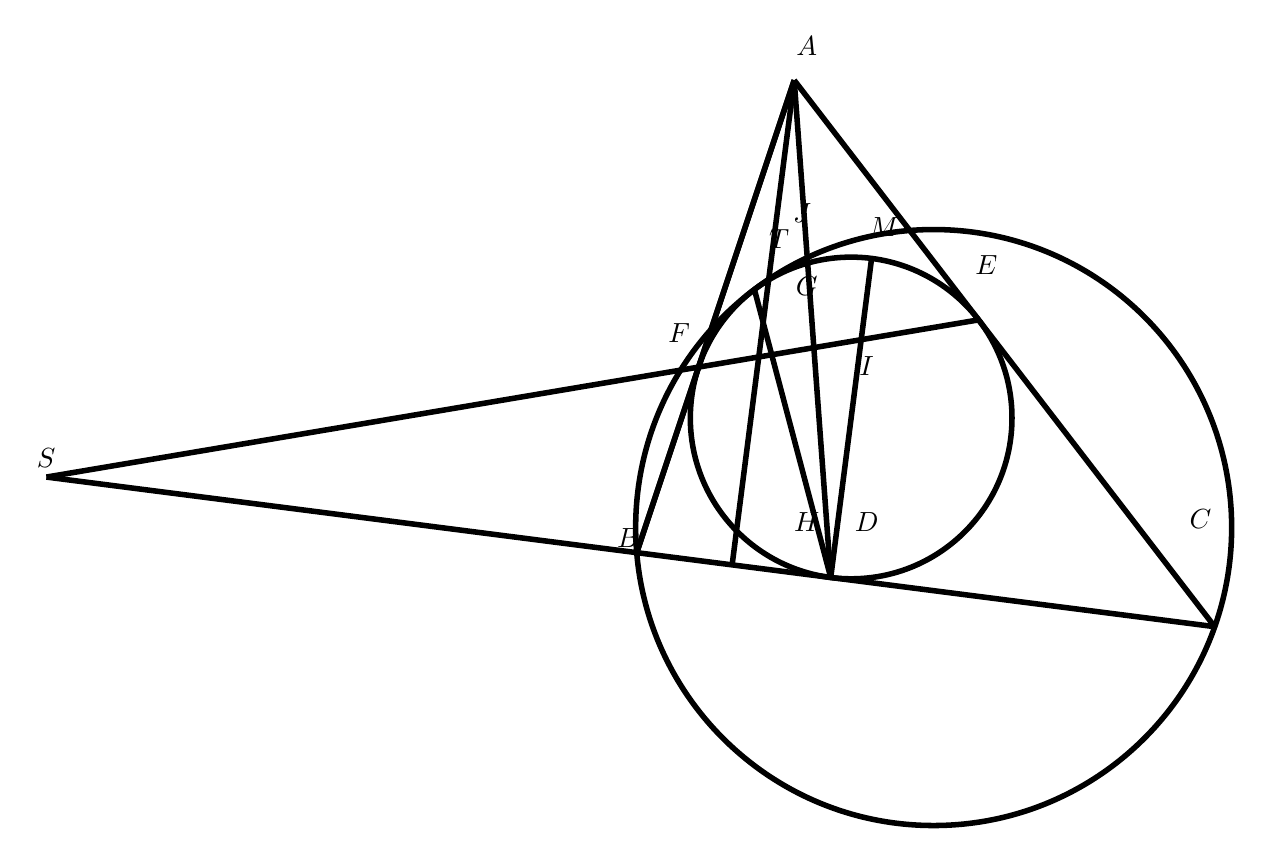
\begin{tikzpicture}
	\draw [line width=2pt] (-2,3)-- (-4,-3);
\draw [line width=2pt] (-2,3)-- (-4,-3);
\draw [line width=2pt] (-4,-3)-- (3.34,-3.94);
\draw [line width=2pt] (3.34,-3.94)-- (-2,3);
\draw [line width=2pt] (-1.2767371404527357,-1.2894752232791138) circle (2.0425985621948755cm);
\draw [line width=2pt] (-2,3)-- (-2.7882657160805855,-3.1551812298207427);
\draw [line width=2pt] (-0.22895941987962345,-2.681023555230252) circle (3.7845069730722622cm);
\draw [line width=2pt] (-2.505383406914281,0.342283716696604)-- (-1.5362042585289566,-3.3155269750657737);
\draw [line width=2pt] (-11.496350612465433,-2.0399768970412118)-- (0.3421020108736435,-0.04385542237136443);
\draw [line width=2pt] (-4,-3)-- (-11.496350612465433,-2.0399768970412118);
\draw [line width=2pt] (-2,3)-- (-1.5362042585289566,-3.3155269750657737);
\draw [line width=2pt] (-1.017270022376515,0.736576528507546)-- (-1.5362042585289566,-3.3155269750657737);
\draw (-1.84,3.43) node {$A$};
\draw (-3.84,-2.57) node [below left] {$B$};
\draw (3.16,-2.57) node {$C$};
\draw (-1.08,-0.63) node {$I$};
\draw (-1.08,-2.61) node {$D$};
\draw (0.44,0.65) node {$E$};
\draw (-3.46,-0.45) node [above] {$F$};
\draw(-1.84,-2.61) node {$H$};
\draw (-1.84,0.39) node {$G$};
\draw (-2.19,0.74) node [above] {$T$};
\draw (-0.86,1.13) node {$M$};
\draw (-1.66,1.07) node [above left] {$J$};
\draw (-11.5,-2.04) node [above] {$S$};
	\end{tikzpicture}
\end{center}
\textbf{Lời giải.} Gọi \(S\) là giao điểm của \(BC\) và \(EF\), \(J\) là giao điểm thứ hai của \(AD\) với đường tròn \(\left( I \right)\), \(M\) là giao điểm của đoạn thẳng \(AI\) và đường tròn \(\left( I \right)\). \\
Ta có: \(D\left( {MGAH} \right) =  - 1\) (chùm điều hòa trung tuyến) nên tứ giác \(MTJD\) là tứ giác điều hòa.\\
\(SJ\) là tiếp tuyến của đường tròn \(\left( I \right)\) do tứ giác \(JFDE\) là tứ giác điều hòa.\\
Nên \(SD\) là tiếp tuyến của \(\left( I \right)\).\\
\( \Rightarrow \) \(S, T, M\) thẳng hàng, mà \(SM \bot TD\) nên \(TD\) là phân giác trong của góc \(\widehat {BTC}.\)\\
Gọi \(L\) là tâm đường tròn ngoại tiếp tam giác \(TBC\), \(Q\) là điểm chính giữa cung \(BC\) không chứa \(T\) của đường tròn này thì \(T, D, Q\) thẳng hàng và \(LQ\) song song với \(ID\).\\
Suy ra: \(\widehat {DTI} = \widehat {TDI} = \widehat {TQL} = \widehat {QTL}.\)\\
Do đó, \(T, I, L\) thẳng hàng. Từ đó, ta có đpcm.\\
\textbf{Nhận xét:} Đây là một bài toán hay và điển hình cho ứng dụng của tứ giác điều hòa xuất hiện trong kì thi Olympic Toán quốc tế, sau đây xin đưa ra một kết quả khác được phát triển dựa trên bài toán trên.\\
\textbf{Ví dụ 12.1} (Đề chọn đội tuyển Hải Phòng 2016 - 2017)\\
 Cho tam giác nhọn \(ABC\), \(\left( AB < AC \right)\), phân giác trong đỉnh \(A\) cắt \(BC\) tại \(D\), \(E\) là điểm trên đoạn \(BC\) sao cho \(BD = BE\). Phân giác ngoài tại đỉnh \(A\) cắt đường thẳng qua \(D\) và vuông góc với \(BC\) tại \(F\). \(I\) là trung điểm của \(DF\), đường thẳng \(EI\) cắt \(AD\) tại \(M\), đường thẳng \(EF\) cắt đường thẳng qua \(M\) và vuông góc với \(BC\) tại \(K\).\\
a. Đường thẳng \(AF\) cắt đường thẳng \(BC\) tại \(P\), \(KD\) cắt đường tròn đường kính \(DF\) tại điểm thứ hai \(L\). Chứng minh rằng đường thẳng \(PL\) tiếp xúc với đường tròn đường kính \(DF\).\\
b. Chứng minh rằng \(I\) là tâm đường tròn nội tiếp tam giác \(KBC\).
\newpage
\section{Bài tập rèn luyện.}
\textbf{Bài 1.} Cho tam giác \(ABC\) có trực tâm \(H\). Gọi \(D\) là giao điểm của \(BH\) và \(AC\), \(E\) là giao điểm của \(CH\) và \(AB\). Đường tròn ngoại tiếp tam giác \(ADE\) cắt đường tròn ngoại tiếp tam giác \(ABC\) tại điểm \(F\) khác \(A\). Chứng minh rằng phân giác trong các góc \(\widehat {BFC},\widehat {BHC}\) cắt nhau tại một điểm trên \(BC\).\\
\textbf{Bài 2.} (IMO 2003) Cho tứ giác \(ABCD\) nội tiếp. Gọi \(P, Q, R\) là lần lượt là chân đường vuông góc kẻ từ \(D\) đến \(BC, CA, AB\). Chứng minh rằng \(PQ = QR\) khi và chỉ khi phân giác các góc \(\widehat {ABC},\widehat {ADC}\) cắt nhau tại một điểm trên \(AC\).\\
\textbf{Bài 3.} Cho tam giác \(ABC\) ngoại tiếp \(\left( I \right)\), \(\left( I \right)\) tiếp xúc với \(BC, CA, AB\) lần lượt tại \(D, E, F\). \(AD\) cắt \(\left( I \right)\) tại điểm thứ hai \(M\).\(BM, CM\) cắt \(\left( I \right)\) lần lượt tại \(Y, Z\). Chứng minh rằng \(BZ, CY, AD\) đồng quy. \\
\textbf{Bài 4.} (Vietnam TST 2002) Trong mặt phẳng cho hai đường tròn \({\omega _1}\) tâm \(O\) và \({\omega _2}\) tâm \(O'\) cắt nhau tại \(A\) và \(B\). Các tiếp tuyến tại \(A, B\) của \({\omega _1}\) cắt nhau tại \(K\). Giả sử \(M\) là một điểm nằm trên \({\omega _1}\) nhưng không trùng với \(A\) và \(B\). Đường thẳng \(AM\) cắt \({\omega _2}\) tại điểm thứ hai \(P\), đường thẳng \(KM\) cắt \({\omega _1}\) tại điểm thứ hai \(C\) và đường thẳng \(AC\) cắt \({\omega _2}\) tại điểm thứ hai \(Q\).\\
a. Chứng minh rằng trung điểm \(PQ\) thuộc đường thẳng \(MC\).\\
b. Chứng minh rằng đường thẳng \(PQ\) luôn đi qua một điểm cố định khi \(M\) thay đổi trên \({\omega _1}\).\\
\textbf{Bài 5.} (China TST 2008) Cho tam giác \(ABC\) nhọn có đường tròn \(\left( I \right)\) nội tiếp. \(M, N\) là trung điểm của cung nhỏ \(AC, AB\) của đường tròn \(\left( O \right)\) ngoại tiếp tam giác \(ABC\), \(D\) là trung điểm của \(MN\). Gọi \(G\) là điểm tùy ý trên cung nhỏ \(BC\) của \(\left( O \right)\). Gọi \({I_1}, {I_2}\) lần lượt là tâm đường tròn nội tiếp của các tam giác \(ABG, ACG\). \(P\) là giao điểm thứ hai của \(\left( O \right)\) và đường tròn ngoại tiếp tam giác \(G{I_1}{I_2}\). Chứng minh rằng \(P, I, D\) thẳng hàng.\\
\textbf{Bài 6.} Cho tam giác \(ABC\) nội tiếp đường tròn \(\left( O \right)\), ngoại tiếp đường tròn \(\left( I \right)\), \(AD\) là đường phân giác trong. \(\left( K \right)\), \(\left( L \right)\) lần lượt là đường tròn nội tiếp tam giác \(ABD, ACD\), \(J\) là tâm đường tròn ngoại tiếp tam giác \(AKL\). \(IJ\) cắt đường tròn ngoại tiếp tam giác \(IKL\) tại \(P\) khác \(I\). Chứng minh rằng tâm đường tròn ngoại tiếp tam giác \(PBC\) nằm trên  \(\left( O \right)\).
\newpage
\section{Tài liệu tham khảo.}
1. Tài liệu chuyên Toán Hình học 10 - Đoàn Quỳnh (chủ biên) - NXB Giáo dục Việt Nam 2011.\\
2. Chuyên đề Tứ giác điều hòa - lớp 10 Toán Khóa 17 - THPT Chuyên Lê Quý Đôn - Bình Định.\\
3. Chuyên đề Tứ giác điều hòa - Nguyễn Việt Hà (THPT Chuyên Lào Cai).\\
4. Chuyên đề Tứ giác điều hòa - Phan Nguyễn Văn Trường, Lục Đình Khánh, Bùi Hà Đăng Quang - Trường Phổ thông Năng khiếu - ĐHQG TPHCM.\\
5. Julielltv Blog (Blog của chuyên Hà Tĩnh) - https://julielltv.wordpress.com\\
6. Chuyên đề Tứ giác điều hòa - diễn đàn Mathcopes (chuyên KHTN).\\
7. dinhtrungphan.blogspot.com/2014/06/bai-toan-1-e-thi-olympic-duyen-hai-bac.html
\newpage
\section{Lời kết}
\textit{Các bạn thân mến, qua những bài tập trên, chúng ta thấy được vẻ đẹp của tứ giác điều hòa trong hình học. Tứ giác điều hòa là một công cụ mạnh giúp chúng ta có thể dễ dàng giải quyết các bài khó, nếu nắm vững kiến thức về tứ giác điều hòa, chúng ta có thể tạo ra nhiều bài toán "hay" và "đẹp".\\
Để hoàn thành chuyên đề này, chúng em nhận được nhiều sự giúp đỡ, quan tâm của mọi người, đặc biệt là thầy Trần Quang Vinh - người đã tận tình hướng dẫn để chúng em có thể hoàn tất chuyên đề. Đây là lần đầu nhóm chúng em làm chuyên đề Toán với nội dung về Tứ giác điều hoa - một chuyên đề hay và quan trọng. Có thể kiến thức cung cấp ở trên chưa thực sự đầy đủ, đôi chỗ bài tập giải chưa đầy đủ, chi tiết như mong muốn nhưng đó đã là nỗ lực trong quá trình tìm hiểu của cả nhóm. Dù vậy, chuyên đề chắc chắn không tránh khỏi những thiếu sót, chúng em rất mong nhận được đóng góp quý báu của các thầy cô và các bạn để kiến thức trong lĩnh vực này của chúng em được hoàn thiện hơn. Hi vọng chuyên đề này sẽ mang lại được nhiều điều bổ ích cho bạn đọc.\\
Xin chân thành cảm ơn!}\\
\begin{flushright}
\textbf{Nhóm tác giả}
\end{flushright}
\end{document}
